% !TEX encoding = UTF-8
\documentclass[a4paper,oneside,titlepage]{book}
\usepackage[italian]{babel}
\usepackage[nouppercase]{frontespizio}

\usepackage{amsmath}
\usepackage{amssymb}
\DeclareMathOperator*{\argmax}{\arg\max}
\DeclareMathOperator*{\argmin}{\arg\min}
\usepackage{enumitem}

\usepackage{graphicx}
\graphicspath{{./immagini/}}
\usepackage{subcaption}

\usepackage{hyperref}
\hypersetup{
    colorlinks=true,
    linkcolor=blue
}
\newcommand{\mail}[1]{\href{mailto:#1}{\texttt{#1}}}

\usepackage{xcolor}
\definecolor{background}{HTML}{F7F7F7}
\usepackage{minted}
\setminted[matlab]{
framesep=2mm,
baselinestretch=1.2,
bgcolor=background,
fontsize=\footnotesize,
breaklines=true,
linenos
}


\begin{document}

\begin{frontespizio}
	\Universita {Verona}
	\Dipartimento {Informatica}
	\Scuola {CdLM in Ingegneria e scienze informatiche}
	\Titolo {Fondamenti di machine learning}
	\Sottotitolo {Riassunto del corso}
	\NCandidato {Creato da}
	\Candidato {Davide Zampieri}
	\Annoaccademico {2020-2021}
\end{frontespizio}

\frontmatter
{
  \hypersetup{linkcolor=black}
  \tableofcontents
}

\mainmatter
\chapter{Introduzione}

\section{Sistemi di riconoscimento}
Lo scopo principale della \textit{pattern recognition} è quello di costruire degli oggetti detti \textit{classificatori}, ovvero delle funzioni che permettano di determinare la natura di un particolare soggetto (detto \textit{pattern}). La procedura per costruire un sistema di riconoscimento si articola in 5 fasi:
\begin{enumerate}
    \item Raccolta dei dati.
    \item Scelta delle features.
    \item Selezione del modello.
    \item Training (addestramento del modello).
    \item Testing (valutazione del modello).
\end{enumerate}
\begin{figure}[htp]
	\centering
	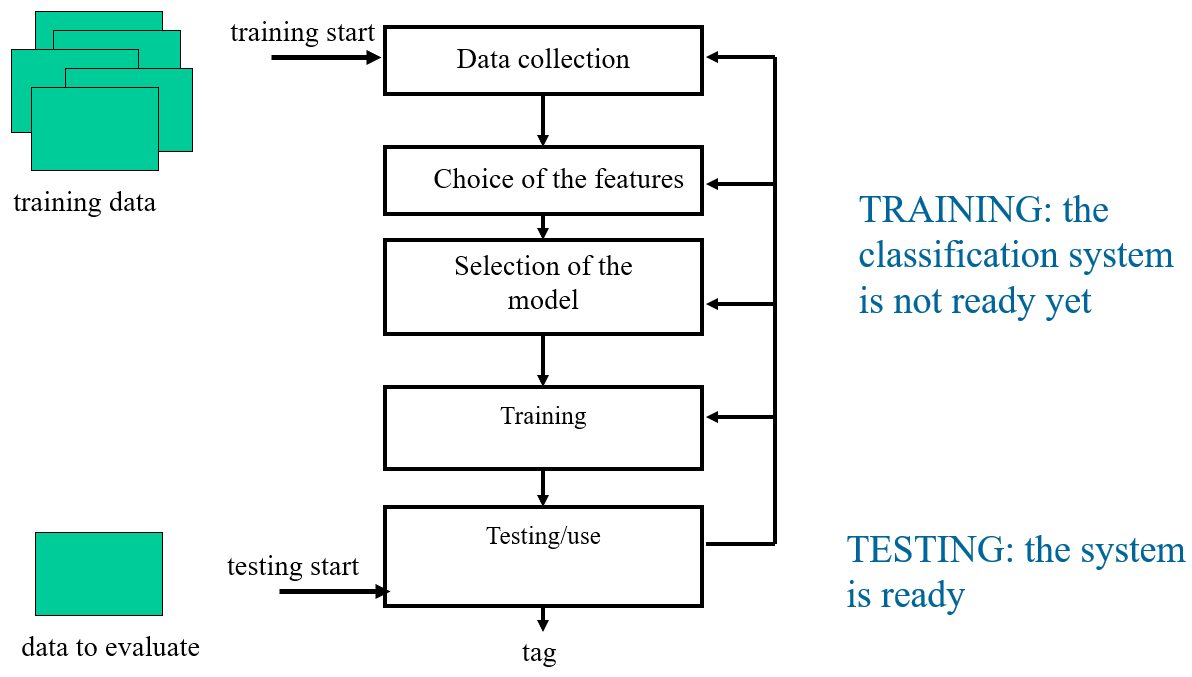
\includegraphics[width=\textwidth, height=\textheight, keepaspectratio]{pr-scheme.png}
\end{figure}

\subsection{Raccolta dei dati}
A seconda dello studio che si vuole fare, utilizzare sensori più o meno precisi può fare la differenza sia per quanto riguarda la chiarezza delle informazioni sia per le dimensioni dei dati stessi. I dati raccolti dovrebbero generare un insieme il più possibile \textit{sufficiente} e \textit{rappresentativo} delle classi che si vogliono studiare.

\subsection{Scelta delle features}
Per scegliere le features più significative si può procedere con la \textit{feature extraction}, ovvero creare nuove features combinando quelle esistenti; oppure, in alternativa, si può procedere con la \textit{feature selection}, ovvero derivare il miglior sottoinsieme delle features immediatamente reperibili dall'osservazione dei dati. 

Le features dovrebbero essere semplici da calcolare, invarianti rispetto a trasformazioni irrilevanti, affidabili, indipendenti, discriminanti e, possibilmente, poche (per il problema dalla \textit{course of dimensionality}).

\subsection{Selezione del modello}
La scelta del modello corrisponde alla scelta della \textit{struttura logica} e delle \textit{basi matematiche} delle regole di classificazione. Lo scopo di un sistema di classificazione (e quindi del classificatore utilizzato) è tipicamente quello di definire il \textit{grado di appartenenza} di un oggetto ad una particolare classe.

Allo stato attuale non esiste un classificatore in grado di spiegare bene tutti i casi di studio; ad esempio le reti neurali sono tra i classificatori più versatili, ma non sono comunque in grado di spiegare ottimamente tutti i possibili fenomeni.

\subsection{Addestramento del modello}
La fase di \textit{training} (detta anche learning) permette di definire la tolleranza e la correttezza di un classificatore. Si parte dall'analisi di un \textit{Training Set} (d'ora in poi TS) di cui si hanno conoscenze a priori, come la natura/classe dei suoi elementi. La fase di training consiste tipicamente nel trovare una variabile di soglia (detta \textit{threshold}) che può essere ad esempio uno scalare, un vettore o una matrice. L'addestramento di un modello di classificazione si divide in tre categorie:
\begin{itemize}
    \item \textit{Addestramento supervisionato} (classificazione), dove l'idea è quella di creare uno strumento in grado di etichettare nuovi oggetti a partire da un TS di cui si conosce la natura degli elementi; i problemi legati a questo approccio sono capire se le soluzioni trovate sono quelle ottimali, capire se lo strumento converge e capire se lo strumento è sufficientemente scalabile (ovvero se la qualità del training è fortemente vincolata al numero di elementi studiati).
    
    \item \textit{Addestramento semi-supervisionato}, dove si effettua un'etichettatura parziale ma significativa (sia in termini di dimensioni che in termini di natura degli oggetti selezionati) del TS e si lascia al classificatore il compito di completare tale operazione; conoscendo a priori il TS è possibile correggere il modello in modo opportuno.
    
    \item \textit{Addestramento non supervisionato} (clustering), dove, in opposizione alla classificazione, si dividono gli oggetti in funzione della somiglianza tra le loro caratteristiche e non in base alla loro natura; questo permette di costruire dei gruppi naturali, i clusters appunto, la cui divisione è fortemente collegata alle caratteristiche prese in considerazione.
    
    \item \textit{Addestramento per rinforzo} (learning with a critic), ovvero una soluzione intermedia alla classificazione e al clustering in cui si procede con una metodologia test-and-try che porta ad un aggiornamento del classificatore mano a mano che si osservano nuovi pattern.
\end{itemize}

\subsection{Valutazione del modello}
In questa fase si valutano le prestazioni del classificatore in termini di \textit{generalizzazione}. Una possibile soluzione al problema di ottenere i migliori risultati di addestramento consiste nel dividere il TS in due: una parte per l'addestramento e l'altra per la validazione (training + validation set). Questo approccio evita il problema dell'\textit{overfitting} (o overtraining) del modello sul TS. Il rischio di un training non controllato porta infatti alla creazione di un classificatore che valuta perfettamente gli elementi del TS ma che alla minima variazione dei valori delle features in un oggetto sconosciuto, rispetto a quelle del TS, sbaglia a classificare. La divisione del TS può procedere per:
\begin{itemize}
    \item \textit{Holdout}, in cui il TS viene suddiviso casualmente in due parti uguali.
    \item \textit{Averaged holdout}, in cui viene fatta una media sul risultato di più partizioni con holdout.
    \item \textit{Leave P-Out}, in cui si effettua il training con tutti i pattern del TS tranne $P$ elementi che vengono usati per il testing; questa procedura viene ripetuta per tutte le combinazioni possibili.
    \item \textit{K-folding} (o Cross-Validation), in cui ogni osservazione viene usata almeno una volta per il testing; questo metodo prevede quindi di testare tutte le combinazioni legate alla suddivisione del TS per poi confrontare i risultati ottenuti.
\end{itemize}
La fase di training necessita di essere fermata prima di incorrere nell'overfitting. Infatti, l'errore di valutazione $E$ di un certo pattern cala con l'avanzare dell'addestramento. Effettuare troppi passi di training porta al superamento di una soglia di generalizzazione $e_0$, con conseguente errore durante la fase di test.
\begin{figure}[htp]
	\begin{subfigure}{0.49\textwidth}
	    \centering
		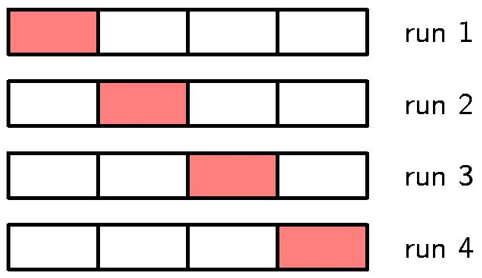
\includegraphics[width=0.75\textwidth]{4-fold.png}
		\caption{K-folding (K = 4)}
	\end{subfigure}
	\hfill
	\begin{subfigure}{0.49\textwidth}
	    \centering
		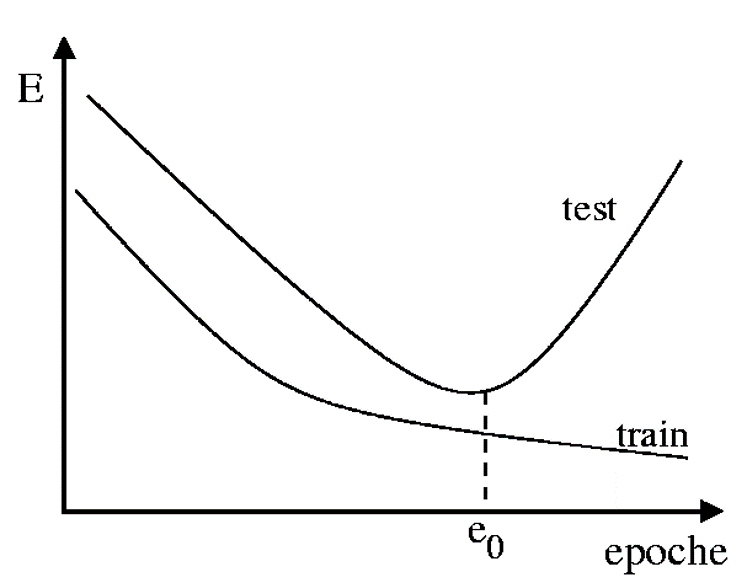
\includegraphics[width=0.75\textwidth]{overtraining.png}
		\caption{Overtraining}
	\end{subfigure}
\end{figure}

\section{Course of dimensionality}
Il problema della \textit{course of dimensionality} è legato al numero di dati del TS che si devono utilizzare per ottenere una classificazione corretta. Infatti, a seconda del numero di features necessarie, il numero di campioni deve essere sufficiente (definito da una relazione
esponenziale) al fine di rappresentare lo spazio delle features nella sua totalità. Si arriva quindi ad una tassellazione dello spazio delle features, in cui gli oggetti del TS devono occupare un sottospazio significativo.
\begin{figure}[htp]
	\centering
	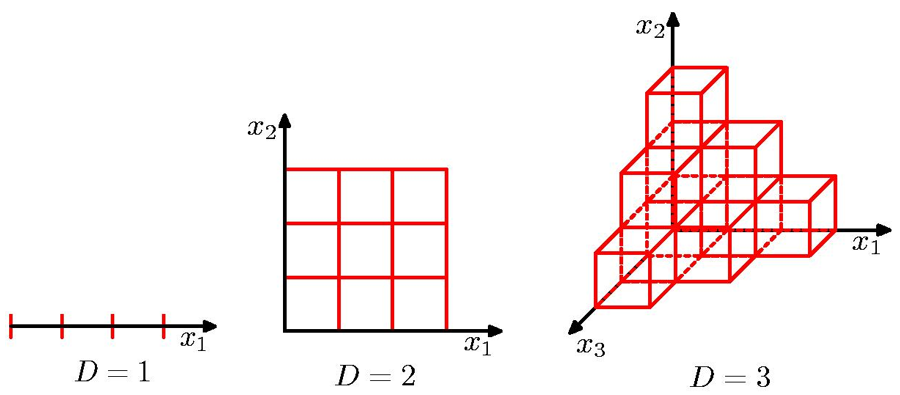
\includegraphics[width=0.9\textwidth]{tassellazione.png}
\end{figure}

\section{Approcci per la pattern recognition}
La pattern recognition può essere affrontata in due modi: tramite un \textit{approccio sintattico}, in cui si considera la struttura dei pattern come la sintassi di un linguaggio; oppure tramite un \textit{approccio statistico}, in cui i pattern sono associati a vettori di features che rappresentano i punti nello spazio mentre tutto il resto è espresso in termini di probabilità.

In quest'ultimo caso si parla di \textit{classificazione statistica} in cui, come abbiamo detto, i pattern sono costituiti da vettori di features e tutte le possibili combinazioni di essi definiscono lo spazio delle features. Se in tale spazio esiste un'ipersuperficie che separa le classi, allora si parla di problema di classificazione a classi separabili.

\section{Classificatore di Bayes}
Alla base dei principi di classificazione c'è il \textit{classificatore di Bayes}, il quale è in grado di dare una descrizione probabilistica delle conoscenze a priori, della bontà del TS e di tutto ciò che riguarda la classificazione.

La \textit{legge di Bayes} calcola la probabilità che un certo oggetto $x$ sia associato ad una determinata classe $C_i$ (probabilità a posteriori, o \textit{posterior}). Tale probabilità è calcolata moltiplicando la probabilità a priori della classe $C_i$ (\textit{prior}) con la \textit{likelihood}, ovvero con la probabilità che la classe descriva correttamente l'oggetto in esame, e dividendo tale prodotto con la \textit{evidence}, ovvero la probabilità con cui $x$ si presenta. Quindi:
\[ P(C_i|x)=\frac{P(C_i) \cdot P(x|C_i)}{P(x)} \]
La probabilità di evidence, invece, è definita come:
\[ P(x) = \sum_{i=1}^N P(C_i) \cdot P(x|C_i) \]

\section{Probability Density Functions}
Il classificatore di Bayes pone le basi ad un grande insieme di approcci per la costruzione di classificatori e algoritmi per le procedure di pattern recognition. Infatti, esistono tre approcci per il calcolo delle \textit{Probability Density Functions} (PDF):
\begin{itemize}
    \item \textit{Classificatori parametrici}, in cui, fissato il modello, tramite il TS si stimano i parametri che rendono ottimale la PDF (ad es. classificatore Gaussiano).
    \item \textit{Classificatori non parametrici}, in cui si tenta di stimare direttamente la PDF basandosi esclusivamente sui dati (ad es. K-Nearest Neighbor).
    \item \textit{Classificatori semi-parametrici}, in cui la classe di modelli della PDF è molto generale e permette di variare il numero di parametri che la definiscono (ad es. reti neurali).
\end{itemize}

\subsection{K-Nearest Neighbor}
Il \textit{KNN} (K-Nearest Neighbor) è un algoritmo che parte dall'idea che oggetti simili saranno vicini (secondo una certa metrica $\Phi$) anche nello spazio delle features. Quindi, dato un oggetto $x_0$ e definito un valore intero positivo e non nullo $K$, si cercano i $K$ elementi più vicini a $x_0$ nello spazio delle features; $x_0$ viene associato alla classe $C$ che si presenta maggiormente tra i $K$ oggetti selezionati. Il problema di questo approccio sta nel definire opportunamente $K$.

\subsection{Reti neurali}
Le \textit{reti neurali} sono sistemi artificiali di elaborazione che emulano il sistema nervoso animale. Si presentano come un modello robusto, compatto, resistente ai guasti e flessibile (si adattano alle nuove situazioni). Inoltre, supportano il calcolo parallelo e permettono di lavorare anche con informazioni incomplete o affette da errore.

Una rete neurale è costituita da: unità elementari chiamate \textit{neuroni}, definiti da una serie di ingressi pesati; un sommatore con la relativa funzione di attivazione; un output. I collegamenti tra neuroni sono detti \textit{sinapsi}. Gli ingressi dei neuroni corrispondono quindi alle features decise dal modello e sono pesati in base all'importanza attribuita a queste ultime. Se i pesi sono associati in modo da costruire un output come combinazione
lineare delle features, allora si può parlare di classificazione probabilistica.

Una rete neurale non permette di osservare direttamente i livelli nascosti, e quindi i processi interni al modello, rendendo difficile lo studio della likelihood (ovvero della descrizione della classe). Un esempio di reti neurali è costituito dalle \textit{feed forward neural networks}.
\begin{figure}[htp]
	\begin{subfigure}{0.49\textwidth}
	    \centering
		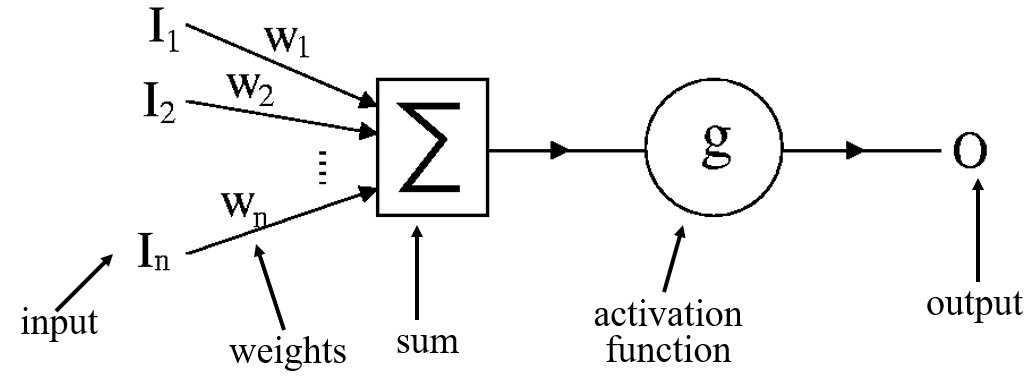
\includegraphics[width=\textwidth, height=\textheight, keepaspectratio]{nn.png}
		\caption{Struttura delle reti neurali}
	\end{subfigure}
	\hfill
	\begin{subfigure}{0.49\textwidth}
	    \centering
		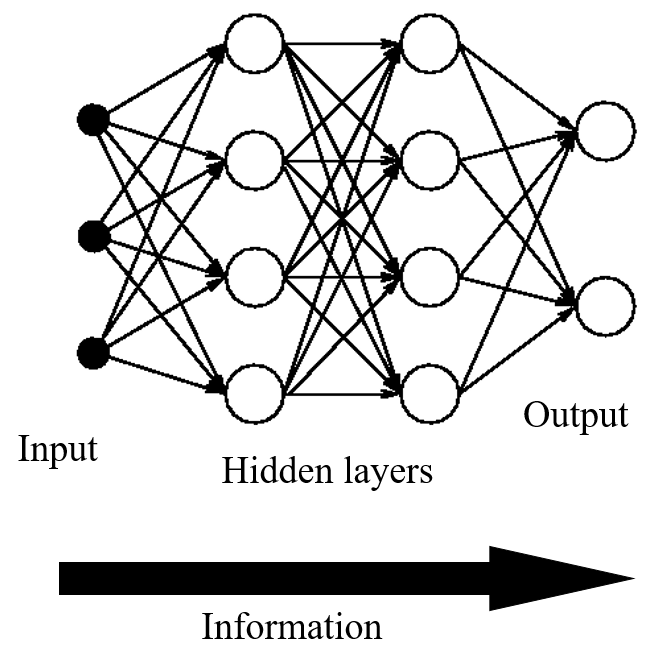
\includegraphics[width=\textwidth, height=\textheight, keepaspectratio]{ffnn.png}
		\caption{Feed forward neural networks}
	\end{subfigure}
\end{figure}

\section{Combinazioni di classificatori}
Esiste la possibilità di effettuare una \textit{combinazione di classificatori}. Infatti, anche se i modelli di classificazione sono costruiti per rispondere ad esigenze specifiche, essi permettono comunque un certo grado di adattamento ai problemi. L'idea è quindi quella di unire vari metodi risolutivi con lo scopo di aumentare le prestazioni di un modello generico. I classificatori possono essere combinati in \textit{parallelo}, in modo \textit{seriale} o in modo \textit{gerarchico}.


\chapter{Teoria della decisione di Bayes}

\section{Introduzione}
La teoria di Bayes è l'approccio statistico fondamentale per la classificazione di patterns. Una volta posto un problema in termini probabilistici e conosciute tutte le \textit{probabilità} rilevanti ad esso associate, si ha l'obiettivo di definire una \textit{regola di decisione} usando le probabilità e i costi associati. La \textit{teoria di Bayes} si basa quindi su quattro concetti probabilistici:
\begin{itemize}
    \item $P(\omega_j) =$ \textit{Prior}, ossia la probabilità di esistenza di una classe nello stato naturale (o spazio di esistenza).
    \item $p(x|\omega_j) =$ \textit{Likelihood}, ossia la probabilità che una certa classe descriva un determinato oggetto (probabilità di misurare $x$ sapendo che lo stato naturale è $\omega_j$).
    \item $p(x) =$ \textit{Evidence}, ossia la probabilità di esistenza di un oggetto (fattore di normalizzazione).
    \item $P(\omega_j|x) =$ \textit{Posterior}, ossia la probabilità che un oggetto sia descritto da una certa classe (formula di Bayes).
\end{itemize}
\begin{figure}[htp]
	\begin{subfigure}{0.49\textwidth}
	    \centering
		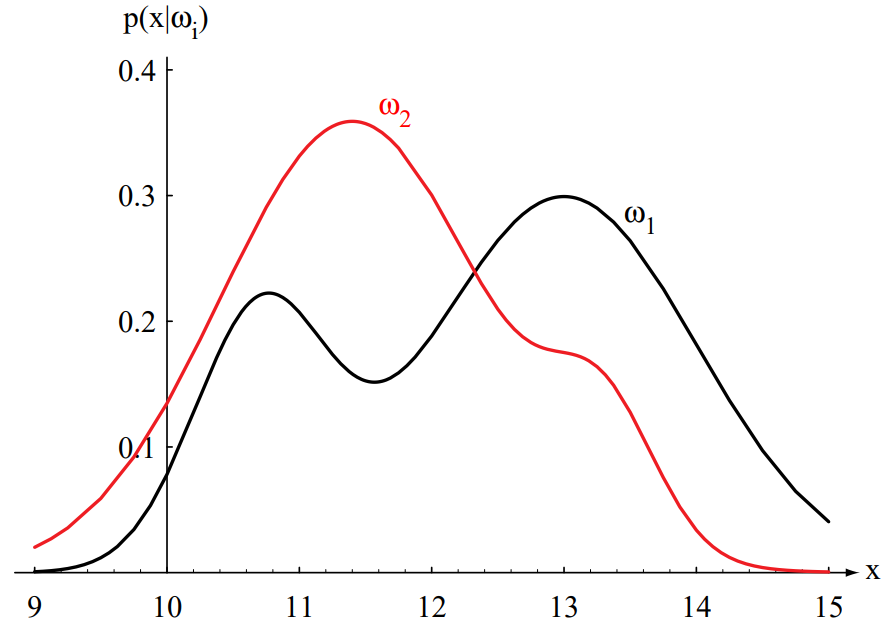
\includegraphics[width=\textwidth, height=\textheight, keepaspectratio]{likelihood.png}
		\caption{Grafico di likelihood (classi $\omega_1$ e $\omega_2$)}
	\end{subfigure}
	\hfill
	\begin{subfigure}{0.49\textwidth}
	    \centering
		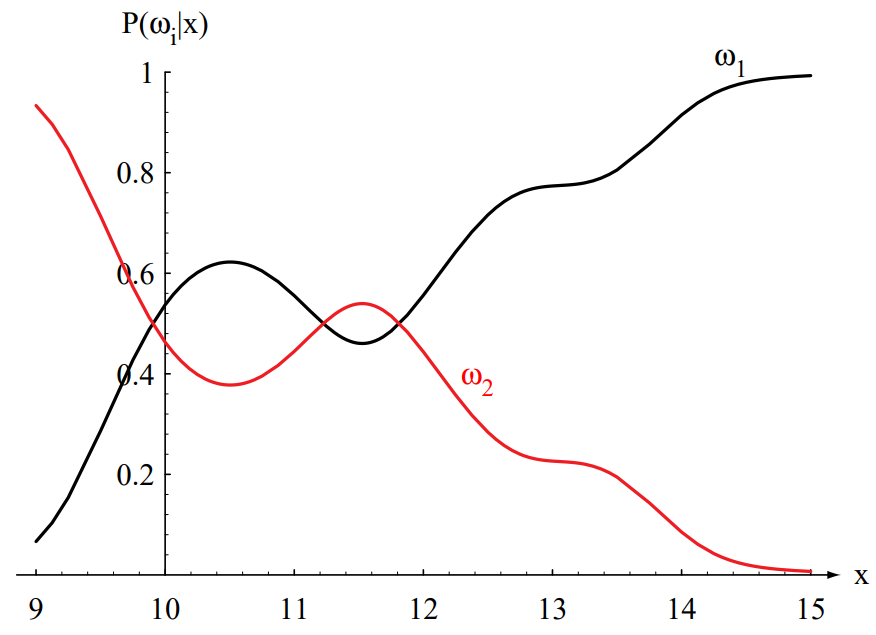
\includegraphics[width=\textwidth, height=\textheight, keepaspectratio]{posterior.png}
		\caption{Grafico di posterior (classi $\omega_1$ e $\omega_2$)}
	\end{subfigure}
\end{figure}

\subsection{Regola di decisione di Bayes}
Dalla formula di Bayes
\[ P(\omega_j|x) = \frac{p(x|\omega_j) \cdot P(\omega_j)}{p(x)} \equiv posterior = \frac{likelihood \cdot prior}{evidence} \]
deriva la \textit{regola di decisione di Bayes}, la quale non è altro che la definizione di una soglia che permetterà di selezionare una classe piuttosto che un'altra. Ovvero:
\begin{center}
    Decide $\omega_1$ if $P(\omega_1|x) > P(\omega_2|x)$, else $\omega_2$
\end{center}

\noindent
La regola di decisione di Bayes minimizza la \textit{probabilità di errore}. Inoltre, rimuovendo la probabilità di evidence, è possibile ottenere una regola di decisione equivalente:
\begin{center}
    Decide $\omega_1$ if $p(x|\omega_1) \cdot P(\omega_1) > p(x|\omega_2) \cdot P(\omega_2)$, else $\omega_2$
\end{center}

\noindent
Infine, esistono due diverse strategie per definire una regola di decisione:
\begin{itemize}
    \item \textit{Approccio generativo}, in cui il problema di decisione si divide in due fasi, una di inferenza (addestramento) e una di decisione (basata sull'uso della probabilità a posteriori).
    \item \textit{Approccio discriminativo}, in cui si genera una funzione (detta funzione discriminante) che permette di classificare gli input mano a mano che vengono letti.
\end{itemize}

\section{Funzione discriminante}
Una \textit{funzione discriminante} è una funzione che divide lo spazio delle features in due semispazi. Quindi, dato un oggetto in ingresso, a seconda del semispazio in cui viene localizzato si può dire se appartiene ad una certa classe o meno. Per ogni classe è infatti definita una particolare funzione discriminante; l'unione delle funzioni discriminanti permette di dividere lo spazio in maniera complessa.

A patto che ci sia \textit{equivalenza}, una funzione discriminante può essere espressa mediante altre funzioni, come il logaritmo. Il motivo di questa operazione sta nella semplicità con cui è possibile trattare certe funzioni rispetto ad altre. Se $g_i$ è la funzione discriminante della classe $\omega_i$ si ha infatti che:
\[ g_i(x) = p(x|\omega_i) \cdot P(\omega_i) = \ln p(x|\omega_i) + \ln P(\omega_i) \]
L'effetto finale delle funzioni discriminanti è quello di partizionare lo spazio delle features in \textit{superfici di separazione} (o di decisione). Tali regioni sono separate dai confini di decisione (\textit{decision boundaries}).
\newpage
\begin{figure}[htp]
	\centering
	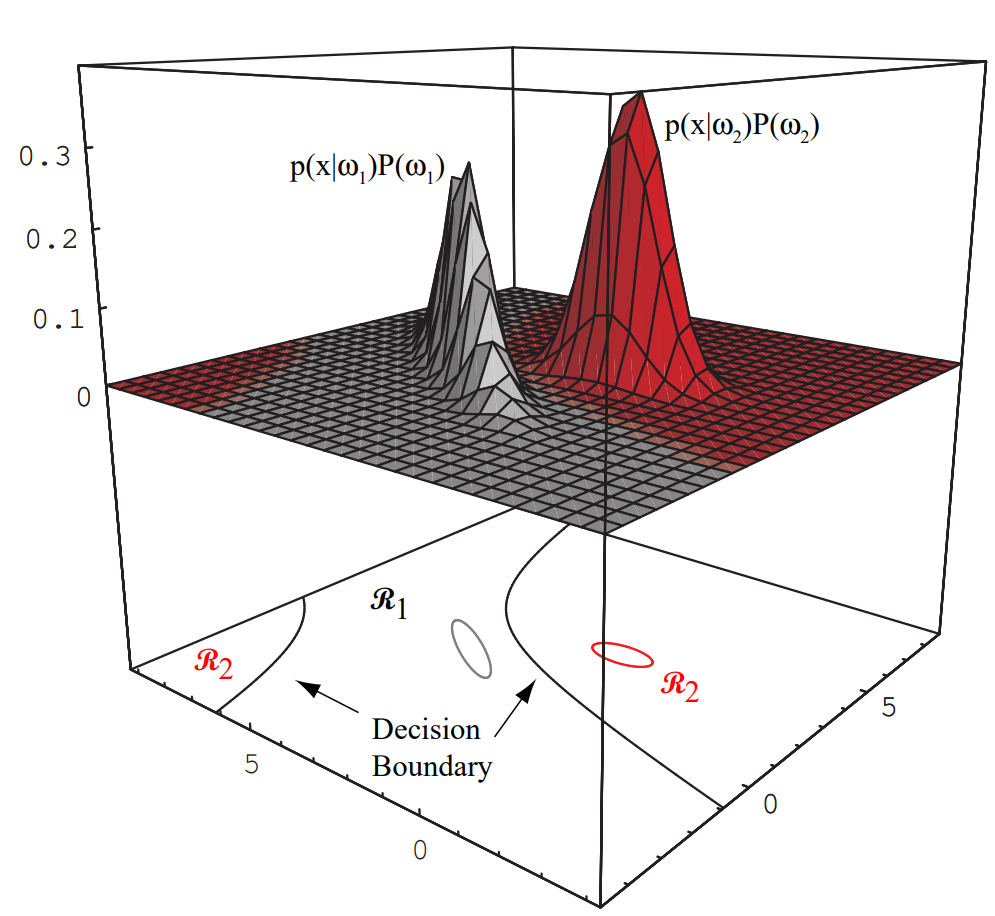
\includegraphics[width=0.9\textwidth]{regioni.png}
\end{figure}

\section{Funzione Gaussiana}
La più importante funzione discriminante, nella teoria di Bayes, è la \textit{funzione Gaussiana} (definita come densità normale o Gaussiana multivariata). Essa infatti è analiticamente trattabile e fornisce la miglior modellazione per problemi sia teorici che pratici. Inoltre, la funzione Gaussiana ha le seguenti \textit{proprietà}:
\begin{itemize}
    \item La sua trasformata di Fourier è sempre una funzione Gaussiana.
    \item Il prodotto di due funzioni Gaussiane è ancora una funzione Gaussiana.
    \item \`{E} ottimale per la localizzazione in tempo o in frequenza.
\end{itemize}

\subsection{Densità normale univariata}
La densità normale \textit{univariata} $N(\mu, \sigma^2)$ è specificata da due parametri: la media e la varianza.
\[ p(x) = \frac{1}{\sqrt{2 \pi} \sigma} \cdot e^{- \frac{1}{2} \left( \frac{x - \mu}{\sigma} \right)^2} \]
\[ \mu \equiv \mathcal{E}[x] = \int_{- \infty}^{\infty} x \cdot p(x) \, dx \]
\[ \sigma^2 \equiv \mathcal{E}[(x - \mu)^2] = \int_{- \infty}^{\infty} (x - \mu)^2 \cdot p(x) \, dx \]
Inoltre, la densità normale è quella dotata di massima entropia, ovvero è in grado di fornire una descrizione più precisa della distribuzione di un certo fenomeno.
\begin{figure}[htp]
	\centering
	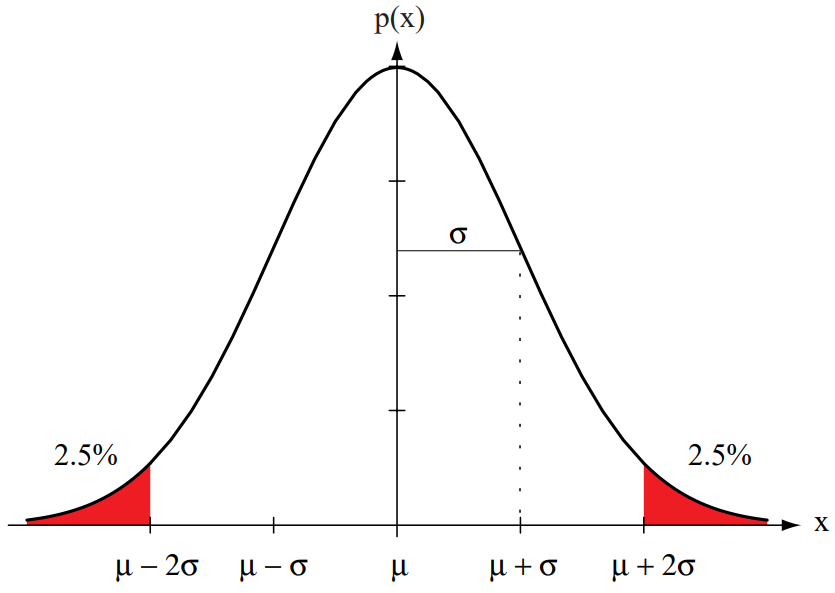
\includegraphics[width=0.6\textwidth]{univariata.png}
\end{figure}

\subsection{Densità normale multivariata}
La densità normale \textit{multivariata} è un'estensione $d$-dimensionale della densità normale univariata, ed è scritta come:
\[ p(x) = \frac{1}{(2 \pi)^{d/2} \cdot |\Sigma|^{1/2}} \cdot e^{- \frac{1}{2} (x - \mu)^t \cdot \Sigma^{-1} \cdot (x - \mu)} \]
dove $\mu$ è un vettore lungo $d$ e $\Sigma$ è la matrice (quadrata) di covarianza di dimensione $d$ che descrive la distribuzione dei punti nello spazio, ovvero il layout della loro disposizione (ipersfere, iperellissi, eccetera). Analiticamente si ha che:
\[ \mu = \frac{1}{N} \cdot \sum_{k=1}^N x^{(k)} \]
\[ \Sigma = \frac{1}{N} \cdot \sum_{k=1}^N (x_i^{(k)} - \mu_i)(x_j^{(k)} - \mu_j) \]
La \textit{matrice di covarianza} $\Sigma$ è simmetrica, semidefinita positiva (determinante maggiore di 0 e autovalori tutti maggiori o uguali a 0) e se due features hanno covarianza nulla questo significa che sono indipendenti. In generale, la matrice di covarianza permette di calcolare la dispersione dei dati in ogni superficie (o sottospazio) descrivendone la distribuzione nello spazio. I suoi autovalori forniscono un valore di dispersione lungo i rispettivi autovettori (assi dello spazio $d$-dimensionale) indicando di fatto l'importanza data ad ogni feature.

L'obiettivo della classificazione sarà quindi quello di trovare la proiezione migliore, ovvero la distanza minore tra un oggetto e una data classe. Quest'ultima viene chiamata \textit{distanza di Mahalanobis} ed è definita come:
\[ r^2 = (x - \mu)^t \cdot \Sigma^{-1} \cdot (x - \mu) \]
Nel caso della normale multivariata, infine, è possibile effettuare una proiezione dello spazio delle features $d$-dimensionale in uno $k$-dimensionale (con $k < d$). Se il prodotto della densità univariata per $x$, componente per componente, è descritto da una distribuzione normale $P(x) = N(\mu, \Sigma)$ e se data una matrice $A_{d,k}$ si ha che $y = A^T \cdot x$ allora
\[ P(y) = N(A^T \cdot \mu, A^T \cdot \Sigma \cdot A) \]
dove $P(y)$ sarà la proiezione di $P(x)$ nello spazio $k$-dimensionale.
\begin{figure}[htp]
	\centering
	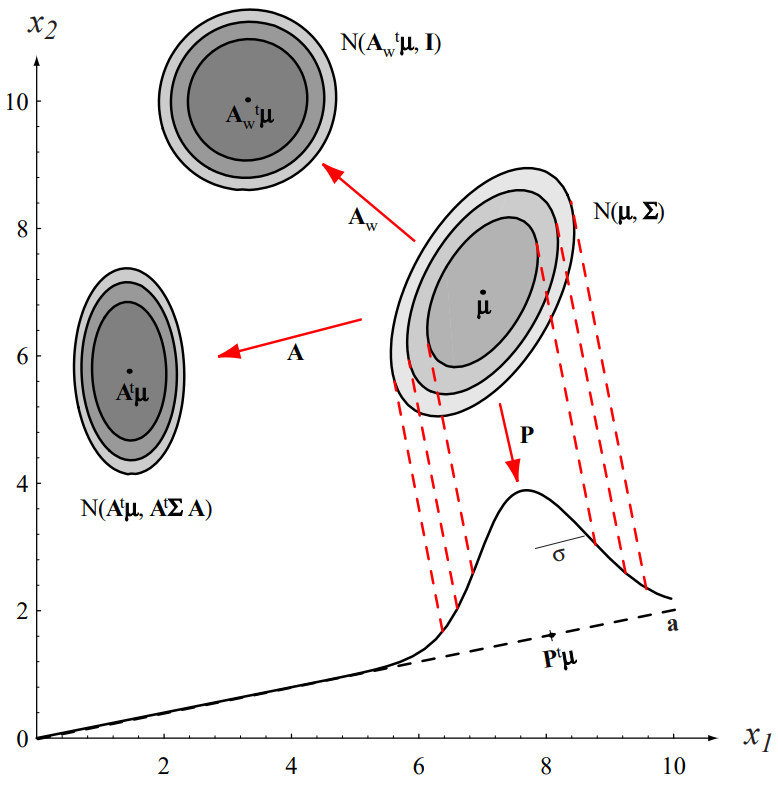
\includegraphics[width=0.75\textwidth]{multivariata.png}
\end{figure}

\section{Funzioni discriminanti - densità normale}
La generica formula per la funzione discriminante nel caso della densità normale è data da $g_i(x)$, la quale si traduce come:
\[ g_i(x) = - \frac{1}{2} (x - \mu_i)^t \Sigma_i^{-1} (x - \mu_i) - \frac{d}{2} \ln 2 \pi - \frac{1}{2} \ln |\Sigma_i| + \ln P(\omega_i) \]

\subsection{Primo caso: \texorpdfstring{$\Sigma_i = \sigma^2 I$}{1-D}}
Nel caso 1-D, in cui la matrice di covarianza è \textit{uguale} per tutte le classi ed è data come $\sigma^2 I$ (ossia quando le features sono indipendenti), la funzione discriminante definisce una retta del tipo $g_i(x) = w_i^t \cdot x + w_{i0}$ dove:
\[ w_i = \frac{1}{\sigma^2} \cdot \mu_i \]
\[ w_{i0} = - \frac{1}{2 \sigma^2} \cdot \mu_i^t \cdot \mu_i + \ln P(\omega_i) \]
Le funzioni di questo tipo sono dette \textit{funzioni discriminanti lineari} o linear machines. Le funzioni discriminanti definiscono generalmente un iperpiano ortogonale alla (iper)linea che unisce le medie delle distribuzioni delle classi. Nel caso in cui le prior risultino uguali, la funzione discriminante si riduce ad un \textit{classificatore di minima distanza}, ovvero si assegna l'elemento $x$ alla classe la cui media $\mu$ è la più vicina all'elemento stesso.
\begin{figure}[htp]
	\begin{subfigure}{0.49\textwidth}
	    \centering
		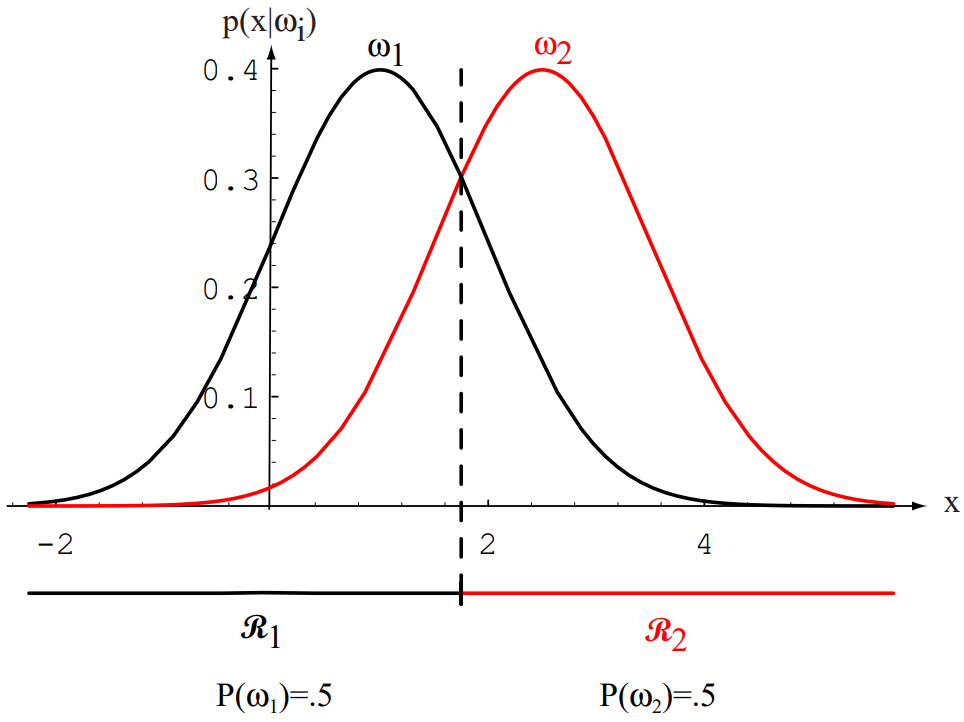
\includegraphics[width=\textwidth, height=\textheight, keepaspectratio]{1D-prior-uguali.png}
		\caption{Linear machine - caso $P(\omega_1) = P(\omega_2)$}
	\end{subfigure}
	\hfill
	\begin{subfigure}{0.49\textwidth}
	    \centering
		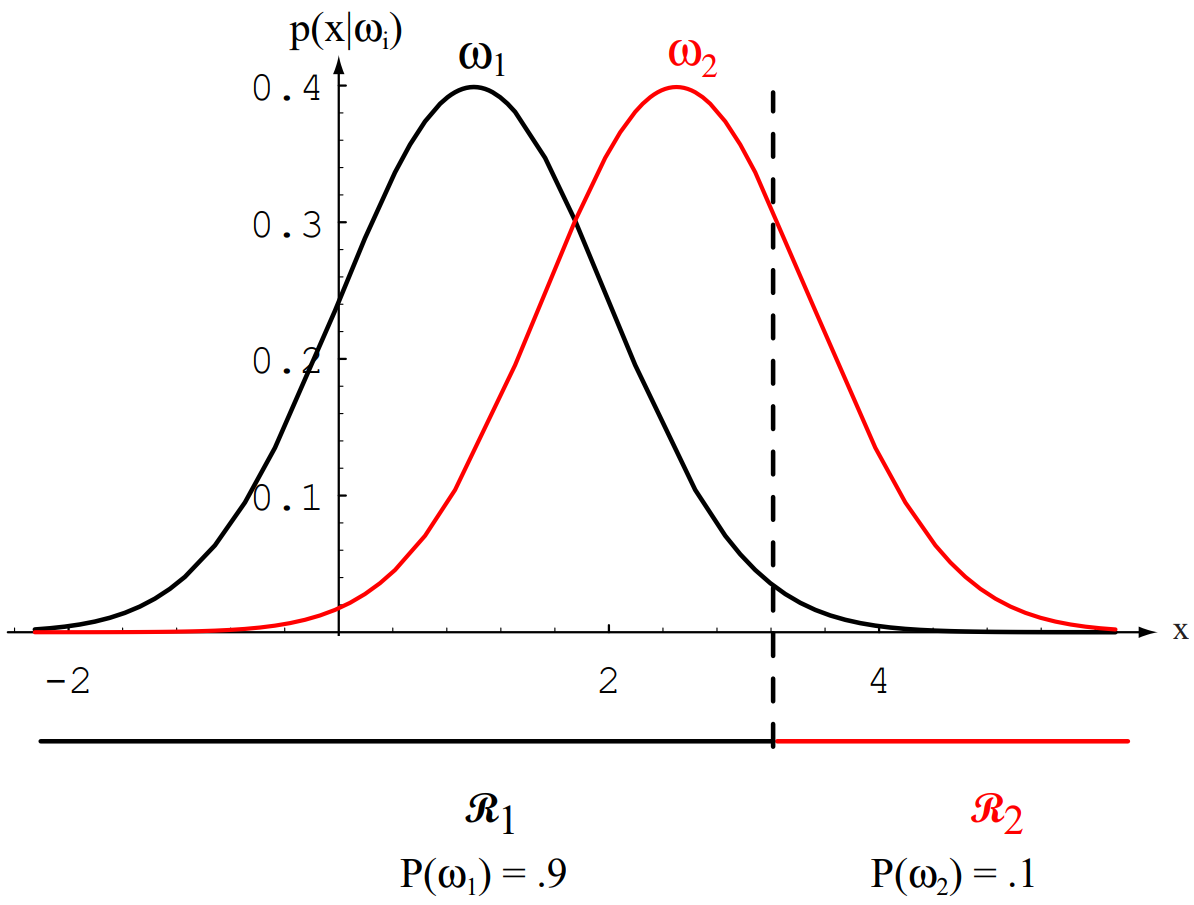
\includegraphics[width=\textwidth, height=\textheight, keepaspectratio]{1D-prior-diversi.png}
		\caption{Linear machine - caso $P(\omega_1) \neq P(\omega_2)$}
	\end{subfigure}
\end{figure}

\subsection{Secondo caso: \texorpdfstring{$\Sigma_i = \Sigma$}{2-D}}
Sempre considerando la densità normale ma nel caso 2-D, in cui la matrice di covarianza è arbitraria ma \textit{uguale} per tutte le classi, $g_i(x)$ può semplificarsi in:
\[ g_i(x) = - \frac{1}{2} (x - \mu_i)^t \Sigma^{-1} (x - \mu_i) + \ln P(\omega_i) \]
Anche in questo caso la funzione discriminante è nella forma di una retta, ma coefficiente angolare e termine noto diventano rispettivamente:
\[ w_i = \Sigma^{-1} \cdot \mu_i \]
\[ w_{i0} = - \frac{1}{2} \cdot \mu_i^t \cdot \Sigma^{-1} \cdot \mu_i + \ln P(\omega_i) \]
Siccome le funzioni discriminanti sono lineari, i \textit{confini di decisione} sono ancora degli iperpiani.
\begin{figure}[htp]
	\centering
	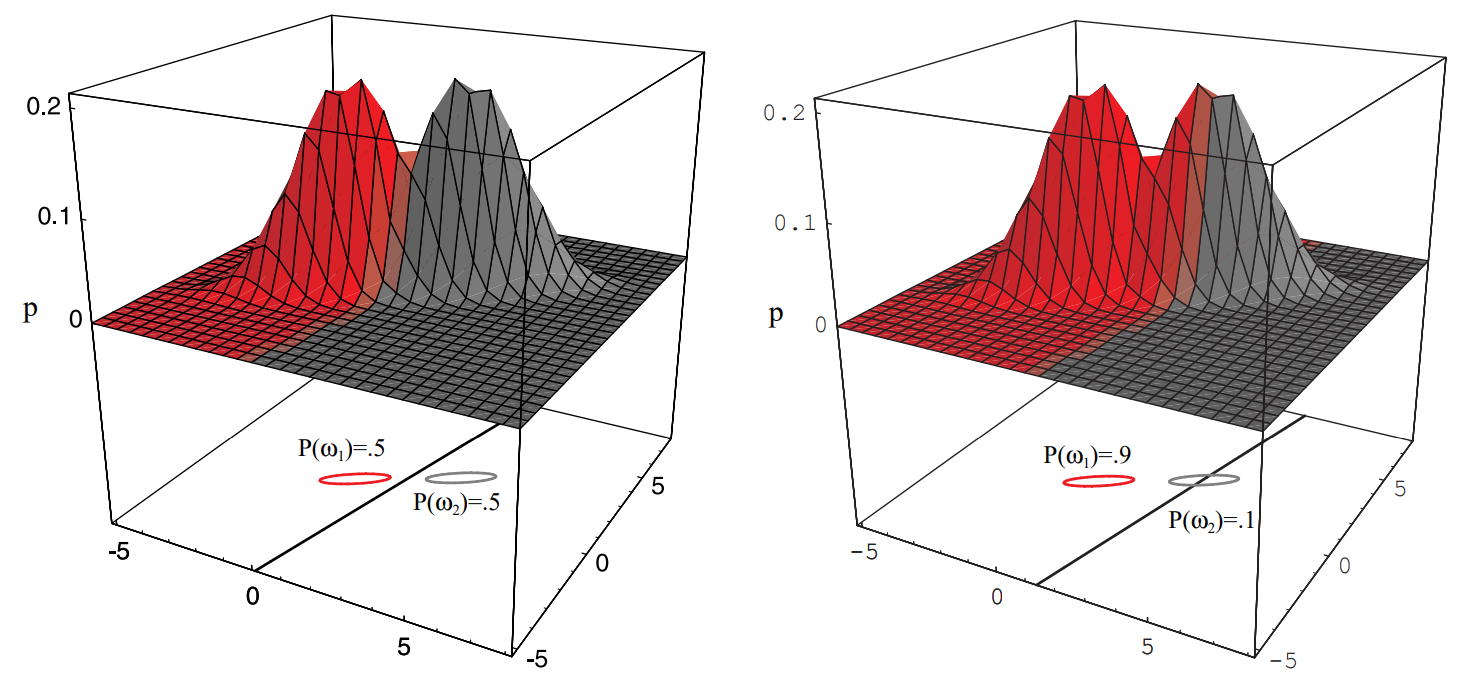
\includegraphics[width=\textwidth, height=\textheight, keepaspectratio]{2D.png}
\end{figure}

\subsection{Terzo caso: \texorpdfstring{$\Sigma_i$}{matrice di covarianza} arbitraria}
In quest'ultimo caso le matrici di covarianza sono \textit{diverse} per ciascuna classe. Le funzioni discriminanti sono quindi intrinsecamente quadratiche:
\[ g_i(x) = x^t \cdot W_i \cdot x + w_i^t \cdot x + w_{i0} \]
dove
\[ W_i = - \frac{1}{2} \cdot \Sigma_i^{-1} \]
\[ w_i = \Sigma_i^{-1}  \cdot \mu_i \]
e
\[ w_{i0} = - \frac{1}{2} \cdot \mu_i^t \cdot \Sigma_i^{-1} \cdot \mu_i - \frac{1}{2} \cdot \ln |\Sigma_i| + \ln P(\omega_i) \]
Nel caso 2-D le \textit{superfici di decisione} sono iperquadratiche e, solitamente, non semplicemente connesse.
\begin{figure}[htp]
	\centering
	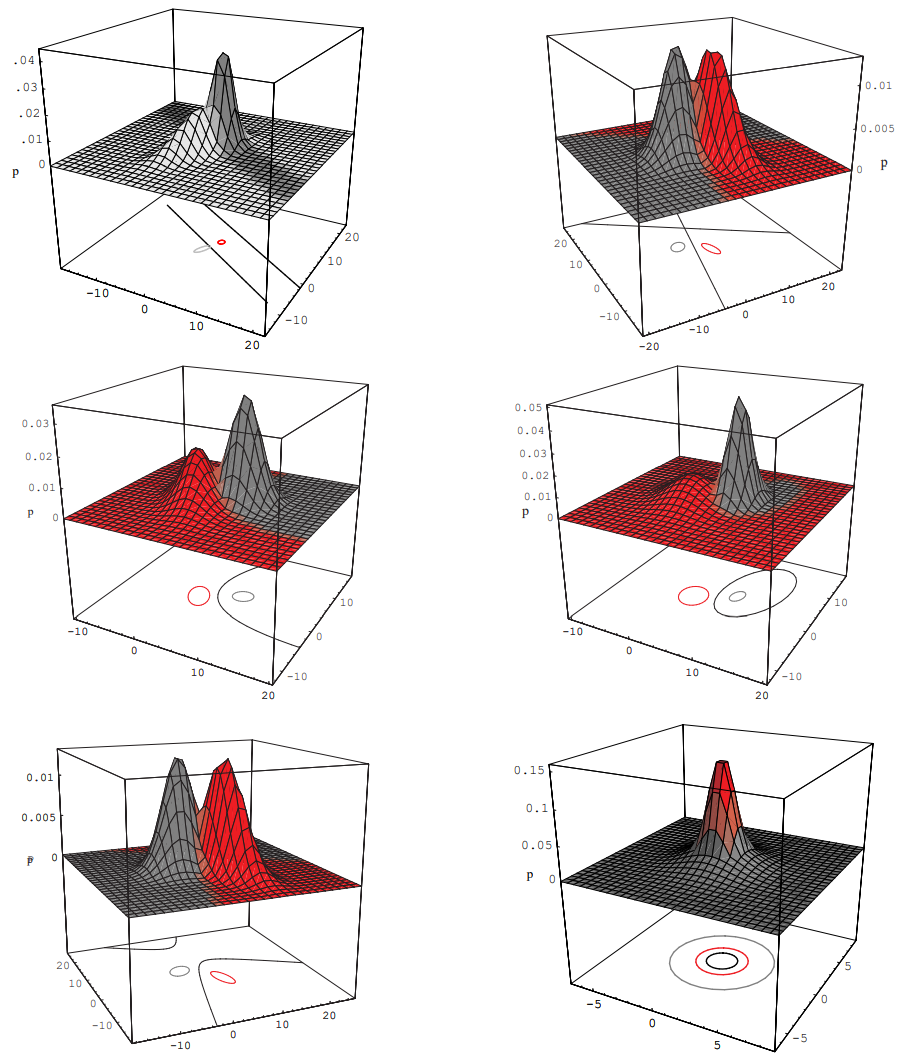
\includegraphics[width=\textwidth, height=\textheight, keepaspectratio]{arbitrary.png}
\end{figure}


\chapter{Estrazione delle features}

\section{Principal Component Analysis}
La \textit{PCA} (Principal Component Analysis), è una tecnica utilizzata per descrivere lo spazio delle features facendone un uso ridotto e semplificandone la struttura, ma garantendo un grado di informazione adeguato al problema studiato.

Dato infatti un vettore N-dimensionale di features, lo scopo della PCA è descrivere in maniera compatta i punti (N-dimensionali) che popolano lo spazio delle features. A seconda del metodo adottato (ad es. \textit{vettore media}) si può incorrere in una rappresentazione poco espressiva e non adeguata a risolvere il problema.

La PCA parte quindi dall'idea di voler proiettare lo spazio delle features in uno spazio dimensionalmente più compatto, costituito dal sottoinsieme di features considerate più significative. Per fare ciò, si vuole calcolare una \textit{retta di regressione}, ovvero una retta su cui proiettare lo spazio, che passa per la media dei punti e che riduce al minimo lo scarto quadratico medio rispetto alla distanza punti-retta. Questo permette di proiettare le coordinate dei punti in uno spazio dimensionalmente più trattabile e, se possibile, con una distribuzione dei dati più facile da analizzare e quindi classificare.
\begin{figure}[htp]
	\begin{subfigure}{0.49\textwidth}
	    \centering
		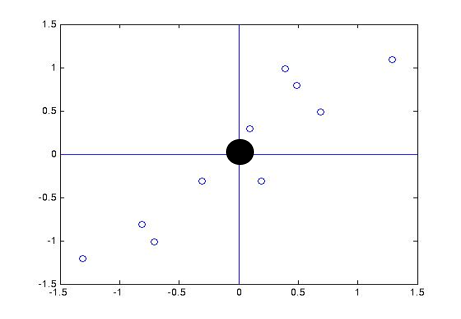
\includegraphics[width=\textwidth, height=\textheight, keepaspectratio]{vettore-media.png}
		\caption{Vettore media}
	\end{subfigure}
	\hfill
	\begin{subfigure}{0.49\textwidth}
	    \centering
		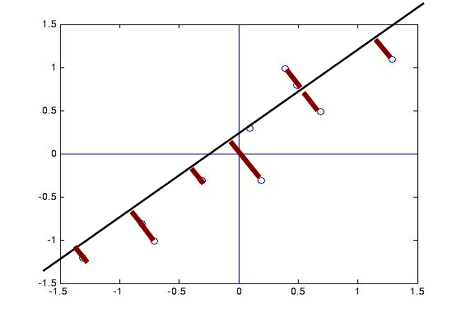
\includegraphics[width=\textwidth, height=\textheight, keepaspectratio]{regressione.png}
		\caption{Retta di regressione}
	\end{subfigure}
\end{figure}

\subsection{Passi formali della PCA}
\begin{enumerate}
    \item Ri-denominazione dei punti per specificare la iper-retta:
    \[ x^{(k)} = m + a^{(k)} \cdot e \]
    \[ \left[ \substack{x_1 \\ \dots \\ x_M} \right] = \left[ \substack{m_1 \\ \dots \\ m_M} \right] + a \cdot \left[ \substack{e_1 \\ \dots \\ e_M} \right] \]
    dove $x$ è il vettore di coordinate (features) di un punto, $m$ è un termine noto che corrisponde alla media dei punti studiati, $a$ è il vettore di coefficienti delle coordinate del punto, mentre $e$ è un vettore unitario che indica la direzione (rispetto alla media) in cui si trova il punto $x$.
    
    \item Trovare i coefficienti $\{ a^{(k)} \}_{k=1 \dots M}$ isolando la variabile $a^{(k)}$:
    \[ a^{(k)} = e^T \cdot (x^{(k)} - m) \]
    
    \item Ottenere il funzionale che descrive il layout degli $M$ punti così da descrivere meglio i punti stessi:
    \[ J_1(e) = - e^T S e + \sum_{k=1}^M \Vert x^{(k)} - m \Vert^2 \]
    
    \item Minimizzare $J_1(e)$ massimizzando $e^T S e$ in cui $S$ è la \textit{scatter matrix} (o matrice di covarianza), la quale indica la variazione tra coppie di variabili aleatorie ed è definita come:
    \[ S = \sum_{k=1}^M (x^{(k)} - m) \cdot (x^{(k)} - m)^T \]
    
    \item Alla fine il termine incognito $e$ sarà un autovettore della matrice di covarianza e, siccome dopo la massimizzazione $e^T S e = \lambda e^T e = \lambda$, $\lambda$ sarà il massimo autovalore.
\end{enumerate}
In sintesi, la formula del funzionale $J_1(e)$ può essere letta come: calcolata la somma degli scarti quadratici, si sottrae un valore calcolato sulla distribuzione spaziale dei punti; massimizzare questo fattore da sottrarre significa che le proiezioni delle features sui nuovi assi saranno molto diverse fra loro; conseguentemente l'errore quadratico sulla distanza dalla retta è minimo.
\begin{figure}[htp]
	\begin{subfigure}{0.49\textwidth}
	    \centering
		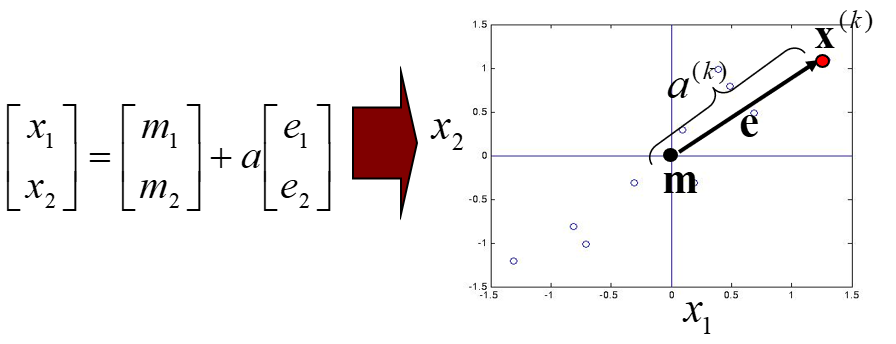
\includegraphics[width=\textwidth, height=\textheight, keepaspectratio]{passo1.png}
		\caption{Ri-denominazione dei punti}
	\end{subfigure}
	\hfill
	\begin{subfigure}{0.49\textwidth}
	    \centering
		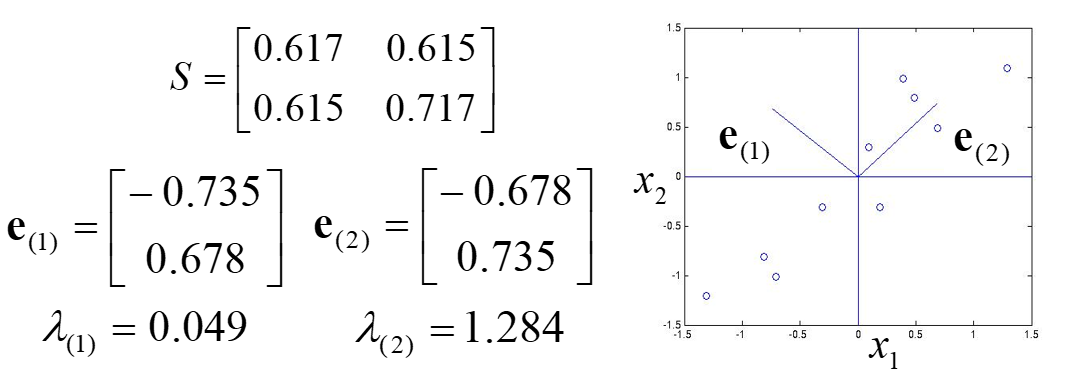
\includegraphics[width=\textwidth, height=\textheight, keepaspectratio]{passo5.png}
		\caption{Autovettori e autovalori}
	\end{subfigure}
\end{figure}

\subsection{Procedura di feature extraction con PCA}
La procedura alla base di PCA si interessa di sapere dove sono i punti (media) e quindi come sono localizzati (retta di proiezione). Le fasi di tale procedura di estrazione delle features sono:
\begin{enumerate}
    \item Si calcola la media dei dati che vivono nello spazio delle features; solitamente si procede con lo spostamento delle classi di oggetti nell'origine per semplificare i calcoli della \textit{matrice di covarianza}.
    \item Presa la matrice di covarianza se ne calcolano \textit{autovettori} e \textit{autovalori}, corrispondenti rispettivamente alle dimensioni dello spazio delle features e ai relativi pesi.
    \item Si decide quali features scartare; ad esempio, una volta normalizzati gli autovalori e disposti in ordine decrescente si seleziona il più grande (o i più grandi). 
\end{enumerate}
Riguardo all'ultima fase si fa notare che gli autovalori più grandi si avranno nelle direzioni di massima dispersione dei dati, ovvero in quelle corrispondenti alle features più significative. Quindi, i corrispondenti autovettori selezionati identificheranno gli \textit{assi} di un sottospazio trasformato in cui sono proiettati i punti.

\subsection{Considerazioni su PCA}
La PCA parte dal presupposto che i dati siano descrivibili tramite una distribuzione gaussiana e con un numero di features \textit{drammaticamente minore} rispetto a quello di partenza. Per soddisfare queste condizioni, i dati devono essere ragionevolmente \textit{simili} nelle condizioni di acquisizione, ovvero non deve essere necessaria alcuna elaborazione particolare per riuscire a distinguere le classi.

\subsection{Esempio in MATLAB}
\begin{minted}{matlab}
load 'irisSet.mat' % X = data, l = labels

% 0: scatters of the 4 features
figure; hold on
subplot(1,4,1);
scatter(0.*X(1,:), X(1,:), 20, l);
title('f. 1');
subplot(1,4,2);
scatter(0.*X(2,:), X(2,:), 20, l);
title('f. 2');
subplot(1,4,3);
scatter(0.*X(3,:), X(3,:), 20, l);
title('f. 3');
subplot(1,4,4);
scatter(0.*X(4,:), X(4,:), 20, l);
title('f. 4');
colormap jet

% Apply PCA on X, in order to have a set of new axis, where each one of them can be sorted depending on the variance it contains
[d,N] = size(X); % number of features, number of points

% 1a: means of the 4 features
u = mean(X,2);

% 1b: centering
h = ones(1,N);
B = X-u*h; % translate the points by the means

% 1c: covariance matrix
C = 1/(N-1) * B*B';

% 2: eigenvectors and eigenvalues
[V,D] = eig(C);

% 3b: sorting eigenvalues
D = diag(D);
[D,ind] = sort(D,'descend');
V = V(:,ind); % V contains the eigenvectors organized by columns (the first column has the largest eigenvector and so on)

% 3b: selecting a single dimension (the largest eigenvector)
V1 = V(:,1);

% 3c: projection
W = V1'*B;

% 4: plot on a single dimension
figure, scatter(ones(1,N),W, 20, l)
set(gcf,'name','1D projection');
colormap jet
\end{minted}
\begin{figure}[htp]
	\begin{subfigure}{0.49\textwidth}
	    \centering
		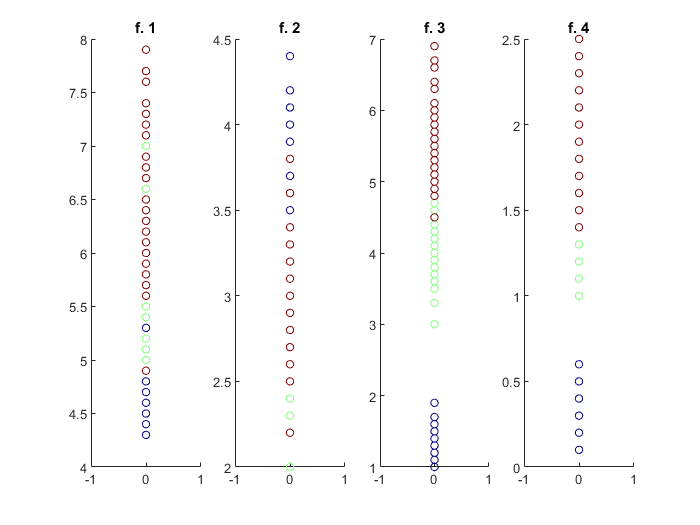
\includegraphics[width=\textwidth, height=\textheight, keepaspectratio]{pca-matlab-1.png}
		\caption{Grafico delle 4 features iniziali}
	\end{subfigure}
	\hfill
	\begin{subfigure}{0.49\textwidth}
	    \centering
		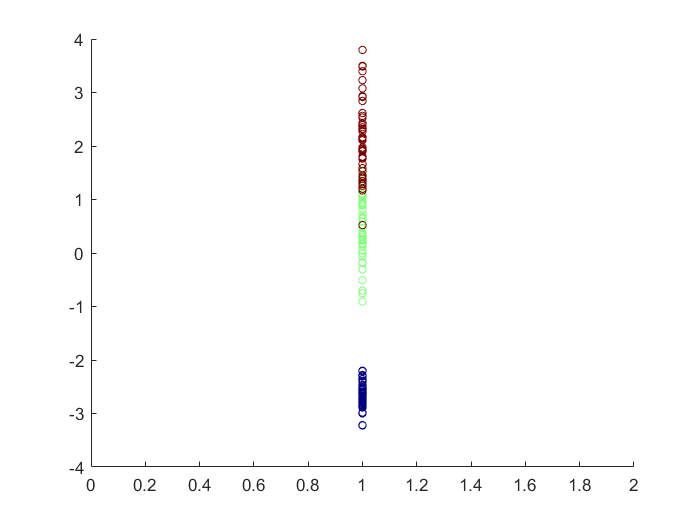
\includegraphics[width=\textwidth, height=\textheight, keepaspectratio]{pca-matlab-2.png}
		\caption{Grafico dei punti proiettati dopo PCA}
	\end{subfigure}
\end{figure}

\subsection{Da PCA alle eigenfaces}
Il problema delle \textit{eigenfaces} è un esempio di applicazione che fa uso di PCA. Una volta ottenuti gli autovettori $e$ (o eigenfaces) dalla matrice di covarianza, posso calcolare le componenti $a$ (o proiezioni) per la faccia $x$ come:
\[ x = m + a_1 e_1 + a_2 e_2 + ... + a_N e_N \]
Gli \textit{autovettori} rappresenteranno quindi varie caratteristiche della faccia (vedi \textit{figura (b)} sottostante).
\begin{figure}[htp]
	\begin{subfigure}{0.49\textwidth}
	    \centering
		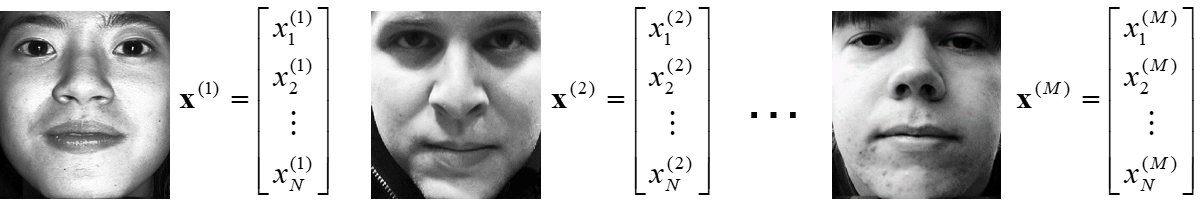
\includegraphics[width=\textwidth, height=\textheight, keepaspectratio]{eigenfaces.png}
		\caption{Dataset di $M$ facce in $N$ dimensioni (con $M << N$)}
	\end{subfigure}
	\hfill
	\begin{subfigure}{0.49\textwidth}
	    \centering
		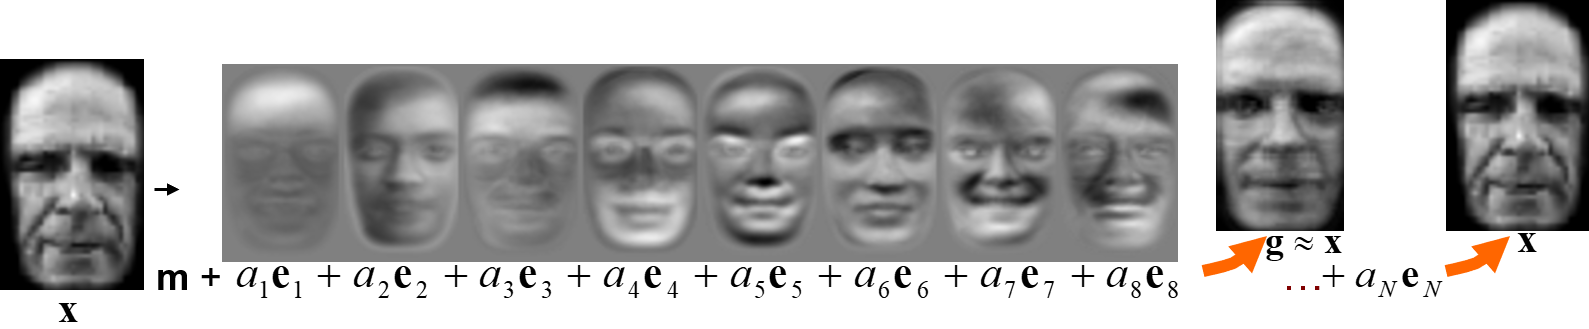
\includegraphics[width=\textwidth, height=\textheight, keepaspectratio]{reconstruction.png}
		\caption{Faccia $x$ e sua ricostruzione $g$}
	\end{subfigure}
\end{figure}

\subsection{Problemi delle eigenfaces}
Se $A$ è una matrice di dimensione $N \times M$, allora la matrice di covarianza $S = A A'$ avrà dimensione $N \times N$. Questo porta a problemi di \textit{overflow}: per un'immagine $256 \times 256$ avrei infatti una matrice $S$ di dimensione $65536 \times 65536$. Il trucco che si può utilizzare per aggirare questo problema consiste nel calcolare gli autovettori come $A' A$ (che ha una dimensione più gestibile pari a $M \times M$) in quanto nelle fasi successive, generalmente, non vengono usate più di 20-30 eigenfaces. Infatti, gli $M$ autovalori di $A' A$ corrispondono agli $M$ autovalori più grandi di $S$:
\[ A' A \tilde{e} = \lambda \tilde{e} \rightarrow A A' A \tilde{e} = \lambda A \tilde{e} \rightarrow S A \tilde{e} = \lambda A \tilde{e} \]
Dal risultato ottenuto si può osservare che $e = A \tilde{e}$.

\subsection{Algoritmo per le eigenfaces}
\begin{enumerate}
    \item Sottrarre da ogni immagine $x^{(k)}$ la media $m = \frac{1}{M} \cdot \sum_{k=1}^M x^{(k)}$.
    \item Costruire la matrice $A$ dai vettori $\tilde{x}^{(k)}$ ottenuti al passo precedente.
    \item Calcolare gli $M$ autovettori $\tilde{e}_i$ di $A' A$ formando la matrice $V$.
    \item Ottenere gli $M$ autovettori più grandi di $S = A A'$ calcolando $e_i = A \tilde{e}_i$ (oppure sotto forma di matrice calcolando $U = A V$).
    \item Ottenere i corrispondenti coefficienti di proiezione calcolando $a_i^{(k)} = e_i' \tilde{x}^{(k)}$ (oppure sotto forma di matrice calcolando $\omega^{(k)} = U' \tilde{x}^{(k)}$).
\end{enumerate}

\section{Linear Discriminant Analysis}
La \textit{Linear Discriminant Analysis} (LDA), o Fisher Discriminant Analysis, è una procedura di features extraction che, come PCA, esegue proiezioni lineari. Rispetto a quest'ultima, tuttavia, offre un grado informativo maggiore sulle classi di oggetti da classificare.

LDA effettua una riduzione delle dimensioni dello spazio delle features con lo scopo di mantenere le classi il più possibile compatte (varianza interna piccola) e distanti fra loro (medie distanti). Lo \textit{spazio delle features} è abitato da $M$ oggetti $N$ dimensionali, ognuno dei quali appartiene ad una delle $i$ classi in cui sono stati partizionati. In LDA ogni classe può quindi contenere un numero variabile di oggetti ma, a differenza di PCA, non si fanno assunzioni sulla loro distribuzione. \`{E} quindi possibile avere casi in cui due o più classi si sovrappongano parzialmente o totalmente.

Come detto, l'obiettivo di LDA è lo stesso di PCA, ovvero si vuole trovare una \textit{proiezione} $w$ tale per cui le coordinate di un punto $x$ siano trasformate in quelle di un punto $y = w^T x$.

\subsection{LDA nel caso di due classi}
Nel caso in cui si trattano due sole classi, $w$ è un vettore con la stessa dimensionalità del punto $x$. Per trovare un buon \textit{vettore di proiezione} è quindi necessario definire una misura di separazione tra le proiezioni. Scegliere l'asse su cui le \textit{medie proiettate} sono le più distanti possibili non risulta ragionevole in un'ottica generale in quanto non tiene conto del layout delle classi. Si potrebbe infatti avere una grande distanza tra \textit{medie}, ma la dispersione dei dati potrebbe causare una sovrapposizione eccessiva. Tutti questi concetti sono rappresentabili analiticamente come:
\[ \mu_i = \frac{1}{M_i} \cdot \sum_{x \in C_i} x \]
\[ \tilde{\mu}_i = \frac{1}{M_i} \cdot \sum_{y \in C_i} y = \frac{1}{M_i} \cdot \sum_{x \in C_i} w^T x = w^T \cdot \frac{1}{M_i} \cdot \sum_{x \in C_i} w^T \mu_i \]
\[ J(w) = |\tilde{\mu}_1 - \tilde{\mu}_2| = |w^T \mu_1 - w^T \mu_2| = |w^T \cdot (\mu_1 - \mu_2)| \]
dove $M_i$ è il numero di oggetti per la classe $C_i$ e $J(W)$ è il funzionale che misura la distanza tra le medie.
\begin{figure}[htp]
	\centering
	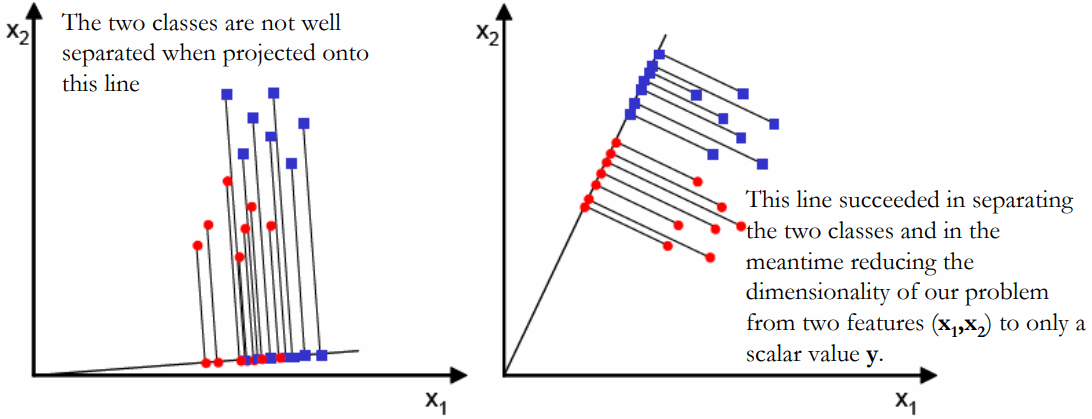
\includegraphics[width=\textwidth, height=\textheight, keepaspectratio]{lda1.png}
\end{figure}

\noindent
L'idea di Fisher è quella di studiare un funzionale che massimizzi la distanza tra le medie, ma che tenga anche conto della distribuzione dei dati. Per questo, per ogni classe, si calcola lo \textit{scatter} nello spazio proiettato
\[ \tilde{s}_i^2 = \sum_{y \in C_i} (y - \tilde{\mu}_i)^2 \]
che rappresenta le informazioni sulla dispersione dei dati rispetto alla relativa media della classe di appartenenza. La somma degli scatter di più classi genera la \textit{within-class} scatter, ovvero una misura della compattezza delle proiezioni delle classi che tiene conto di quanto esse siano compatte in termini spaziali (indipendentemente dalle medie). La LDA è quindi una funzione lineare $w^T x$ che massimizza la funzione criterio
\[ J(w) = \frac{|\tilde{\mu}_1 - \tilde{\mu}_2|^2}{\tilde{s}_1^2 + \tilde{s}_2^2} \]
la quale mostra chiaramente come la massimizzazione sia data nel momento in cui la within-class scatter è piccola (classi compatte) e le medie sono distanti (classi ben separate).
\begin{figure}[htp]
	\centering
	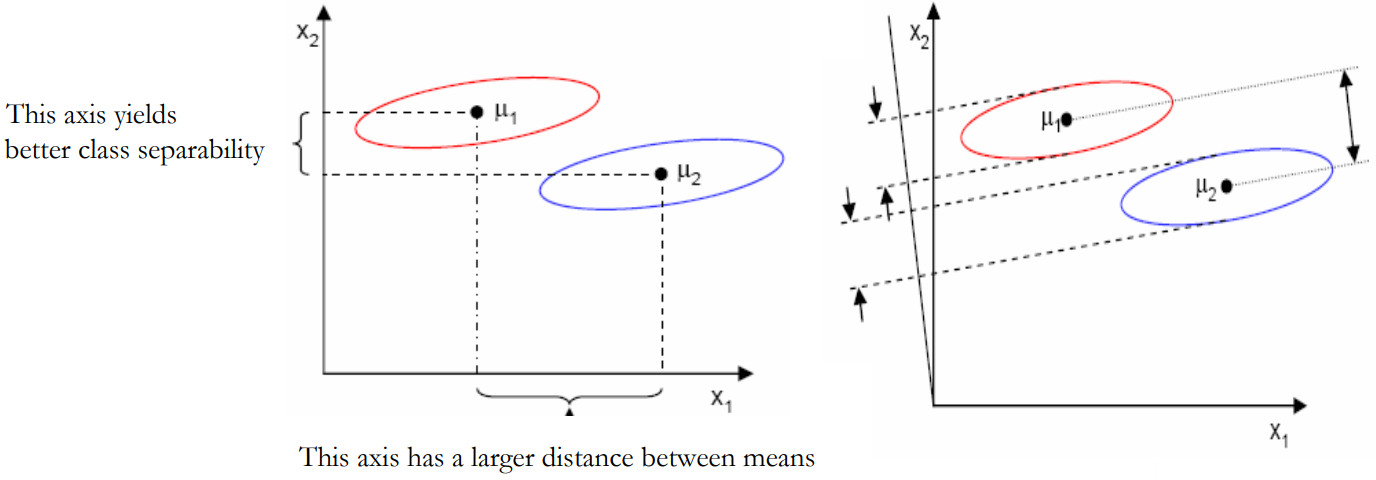
\includegraphics[width=\textwidth, height=\textheight, keepaspectratio]{lda2.png}
\end{figure}

\noindent
Per trovare la \textit{proiezione ottimale} $w^*$, dobbiamo esprimere $J(w)$ come funzione esplicita di $w$. Calcoliamo quindi la within-class scatter matrix $S_W$ definita come somma delle matrici scatter delle singole classi $S_W = S_1 + S_2$, dove:
\[ S_i = \sum_{x \in C_i} (x - \mu_i) \cdot (x - \mu_i)^T \]
Ne consegue che
\[ \tilde{s}_i^2 = \sum_{x \in C_i} (w^T x - w^T \mu_i)^2 = \sum_{x \in C_i} w^T (x - \mu_i) (x - \mu_i)^T w = w^T S_i w \]
da cui deriviamo la within-class scatter matrix dello spazio proiettato:
\[ \tilde{s}_1^2 + \tilde{s}_2^2 = w^T S_1 w + w^T S_2 w = w^T (S_1 + S_2) w = w^T S_W w = \tilde{S}_W \]
Allo stesso modo è possibile calcolare la \textit{between-class} scatter matrix che mostra la distribuzione delle classi nello spazio proiettato:
\[ (\tilde{\mu}_1 - \tilde{\mu}_2)^2 = (w^T \mu_1 - w^T \mu_2)^2 = w^T (\mu_1 - \mu_2) (\mu_1 - \mu_2)^T w = w^T S_B w = \tilde{S}_B \]
A partire da queste considerazioni, si può riscrivere il funzionale come:
\[ J(w) = \frac{w^T S_B w}{w^T S_W w} \]
Massimizzando il criterio di Fisher si riesce a comprendere che è possibile ridursi ad uno spazio con al più $i-1$ dimensioni, dove $i$ è il numero di classi. La \textit{proiezione ottimale} sarà quindi data come:
\[ w^* = \argmax_w J(w) = \argmax_w \left( \frac{w^T S_B w}{w^T S_W w} \right) \]

\subsection{LDA nel caso di \textit{C} classi}
Nel caso in cui si stia considerando un numero di classi $C > 2$ è possibile generalizzare il calcolo delle matrici di scatter in questo modo:
\[ S_W = \sum_{i = 1}^C S_i \]
\[ S_B = \sum_{i = 1}^C M_i (\mu_i - \mu) (\mu_i - \mu)^T \]
dove
\[ S_i = \sum_{x \in C_i} (x - \mu_i) \cdot (x - \mu_i)^T \]
\[ \mu_i = \frac{1}{M_i} \cdot \sum_{x \in C_i} x \]
\[ \mu = \frac{1}{M} \cdot \sum_{\forall x} x = \frac{1}{M} \cdot \sum_{\forall x} M_i \mu_i \]
\begin{figure}[htp]
	\centering
	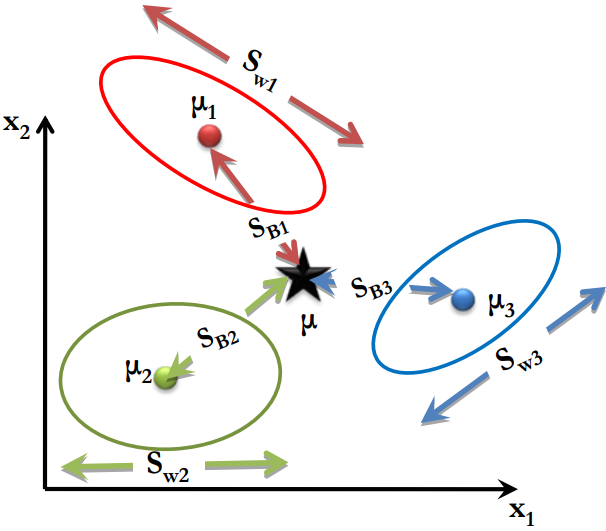
\includegraphics[width=0.75\textwidth]{lda3.png}
\end{figure}

\subsection{Esempio in MATLAB}
\begin{minted}{matlab}
load 'irisSet.mat' % X = data, l = labels

% 0: 2D projection
figure; hold on
subplot(2,3,1);
scatter(X(1,:),X(2,:), 20, l);
title('f. 1,2 ');
subplot(2,3,2);
scatter(X(3,:),X(4,:), 20, l);
title('f. 3,4 ');
subplot(2,3,3);
scatter(X(1,:),X(3,:), 20, l);
title('f. 1,3 ');
subplot(2,3,4);
scatter(X(1,:),X(4,:), 20, l);
title('f. 1,4 ');
subplot(2,3,5);
scatter(X(2,:),X(4,:), 20, l);
title('f. 2,4 ');
subplot(2,3,6);
scatter(X(2,:),X(3,:), 20, l);
title('f. 2,3');
colormap jet

% Apply LDA on X
[d,N] = size(X); % number of features, number of points
K = length(unique(l)); % number of classes

% 1: collect the classes Ck
for k = 1:K
    a = find(l == k);
    Ck{k} = X(:,a);
end

% 2: compute the means
for k = 1:K
    mk{k} = mean(Ck{k},2);
end

% 3: get the cardinalities (for the scatter matrices)
for k = 1:K
    [d, Nk(k)] = size(Ck{k});
end

% 4: within-class covariance for compactness estimation
for k = 1:K
    S{k} = zeros(d,d);
    for i = 1:Nk(k)
        S{k} = S{k} + (Ck{k}(:,i)-mk{k})*(Ck{k}(:,i)-mk{k})';
    end
    S{k} = S{k}./Nk(k);
end
Swx = zeros(d,d);
for k = 1:K
    Swx = Swx + S{k};
end

% 5: between-class covariance
m = mean(X,2);
Sbx = zeros(d,d);
for k=1:K
    Sbx = Sbx + Nk(k)*((mk{k} - m)*(mk{k} - m)');
end

% 6: compute the LDA projection
MA = inv(Swx)*Sbx;

% 7: projection vector
[V,D] = eig(MA);
W = V(:,1:2);
Y = W'*X;

% 8: plot
figure, scatter(Y(1,:),Y(2,:),[],l)
set(gcf,'name','LDA 2D projection');
colormap jet
\end{minted}
\begin{figure}[htp]
	\begin{subfigure}{0.49\textwidth}
	    \centering
		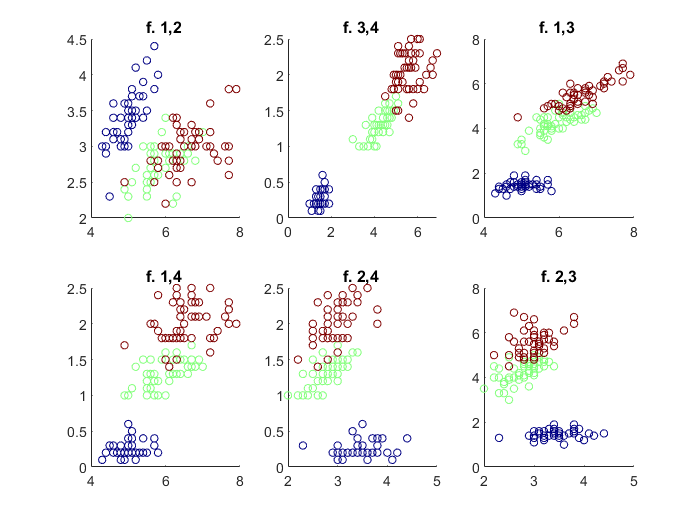
\includegraphics[width=\textwidth, height=\textheight, keepaspectratio]{lda-matlab-1.png}
		\caption{Grafico delle 4 features iniziali}
	\end{subfigure}
	\hfill
	\begin{subfigure}{0.49\textwidth}
	    \centering
		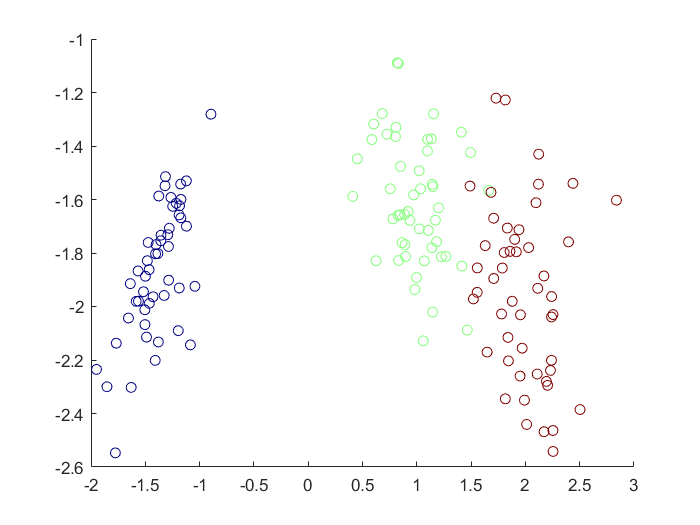
\includegraphics[width=\textwidth, height=\textheight, keepaspectratio]{lda-matlab-2.png}
		\caption{Grafico dei punti proiettati dopo LDA}
	\end{subfigure}
\end{figure}

\subsection{Fisherfaces: algoritmo ed esempio in MATLAB}
\begin{enumerate}
    \item Fare PCA per passare da una matrice $AA$ di dimensione $N \times M$ ($M$ oggetti $N$ dimensionali) ad una matrice $X$ di dimensione $low\_dim \times M$.
    \item Fare LDA per passare dalla matrice $X$ ad una matrice $MA$ di dimensione $low\_dim \times low\_dim$.
    \item Calcolare i $low\_dim$ autovettori di $MA$ e tenerne i primi $C-1$ (con $C$ numero delle classi).
    \item Fare la proiezione (vedere la figura alla fine del codice per un esempio di risultato).
\end{enumerate}
\begin{minted}{matlab}
dire    =    '.\images'; % path of a directory containing 400 bitmap images
list    =   dir(strcat(dire,'\*.bmp'));
M       =   size(list,1);
tmp     =   imread(strcat(dire,'\',list(1).name));
[r,c]   =   size(tmp);
TMP     =   zeros(r*c,M);
for i=1:M
    tmp = imread(strcat(dire,'\',list(i).name));
    TMP(:,i) = tmp(:);
end
TMP     =   double(TMP);

% 0: perform PCA (N x M -> low_dim x M)
media       =   mean(TMP,2);
AA(:,:)     =   TMP-repmat(media,1,M);
[U,lambda]  =   eigen_training(AA); % A'A trick

T           =   200; % low_dim
X           =   U(:,1:T)'*AA; % projection
l           =   reshape(repmat([1:40],10,1),400,1);

% LDA code (low_dim x M -> low_dim x low_dim)
[d,N] = size(X);
K = max(l);
for k = 1:K                     % 1
    a = find(l == k);
    Ck{k} = X(:,a);
end
for k = 1:K                     % 2
    mk{k} = mean(Ck{k},2);
end
for k = 1:K                     % 3
    [d, Nk(k)] = size(Ck{k});
end
for k = 1:K                     % 4
    S{k} = 0;
    for i = 1:Nk(k)
        S{k} = S{k} + (Ck{k}(:,i)-mk{k})*(Ck{k}(:,i)-mk{k})';
    end
    S{k} = S{k}./Nk(k);
end
Swx = 0;
for k = 1:K
    Swx = Swx + S{k};
end
m = mean(X,2);                  % 5
Sbx = 0;
for k=1:K
    Sbx = Sbx + Nk(k)*((mk{k} - m)*(mk{k} - m)');
end
Sbx = Sbx/K;
MA = inv(Swx)*Sbx;              % 6

% C = 40 classes
% take the first 39 eigenvectors (C-1)
[V,D] = eig(MA);
W = V(:,1:39);
Y = W'*X;                       % 7

% 8: plot
figure, scatter(Y(1,:),Y(2,:),[],l)
for i=1:M
    text(Y(1,i),Y(2,i),num2str(l(i)))
end


function [U,lambda] = eigen_training(A)

M             =   size(A,2);
N             =   size(A,1);
L             =   A'*A;

% eigenvectors and eigenvalues of A'A
[V,values]    =   eig(L);
values        =   diag(values);
[lambda, ind] =   sort(values,'descend');
V             =   V(:,ind);

% eigenvectors of AA'
U             =   A*V;
for i=1:M
    U(:,i)=U(:,i)/norm(U(:,i));
end

end
\end{minted}
\begin{figure}[htp]
	\centering
	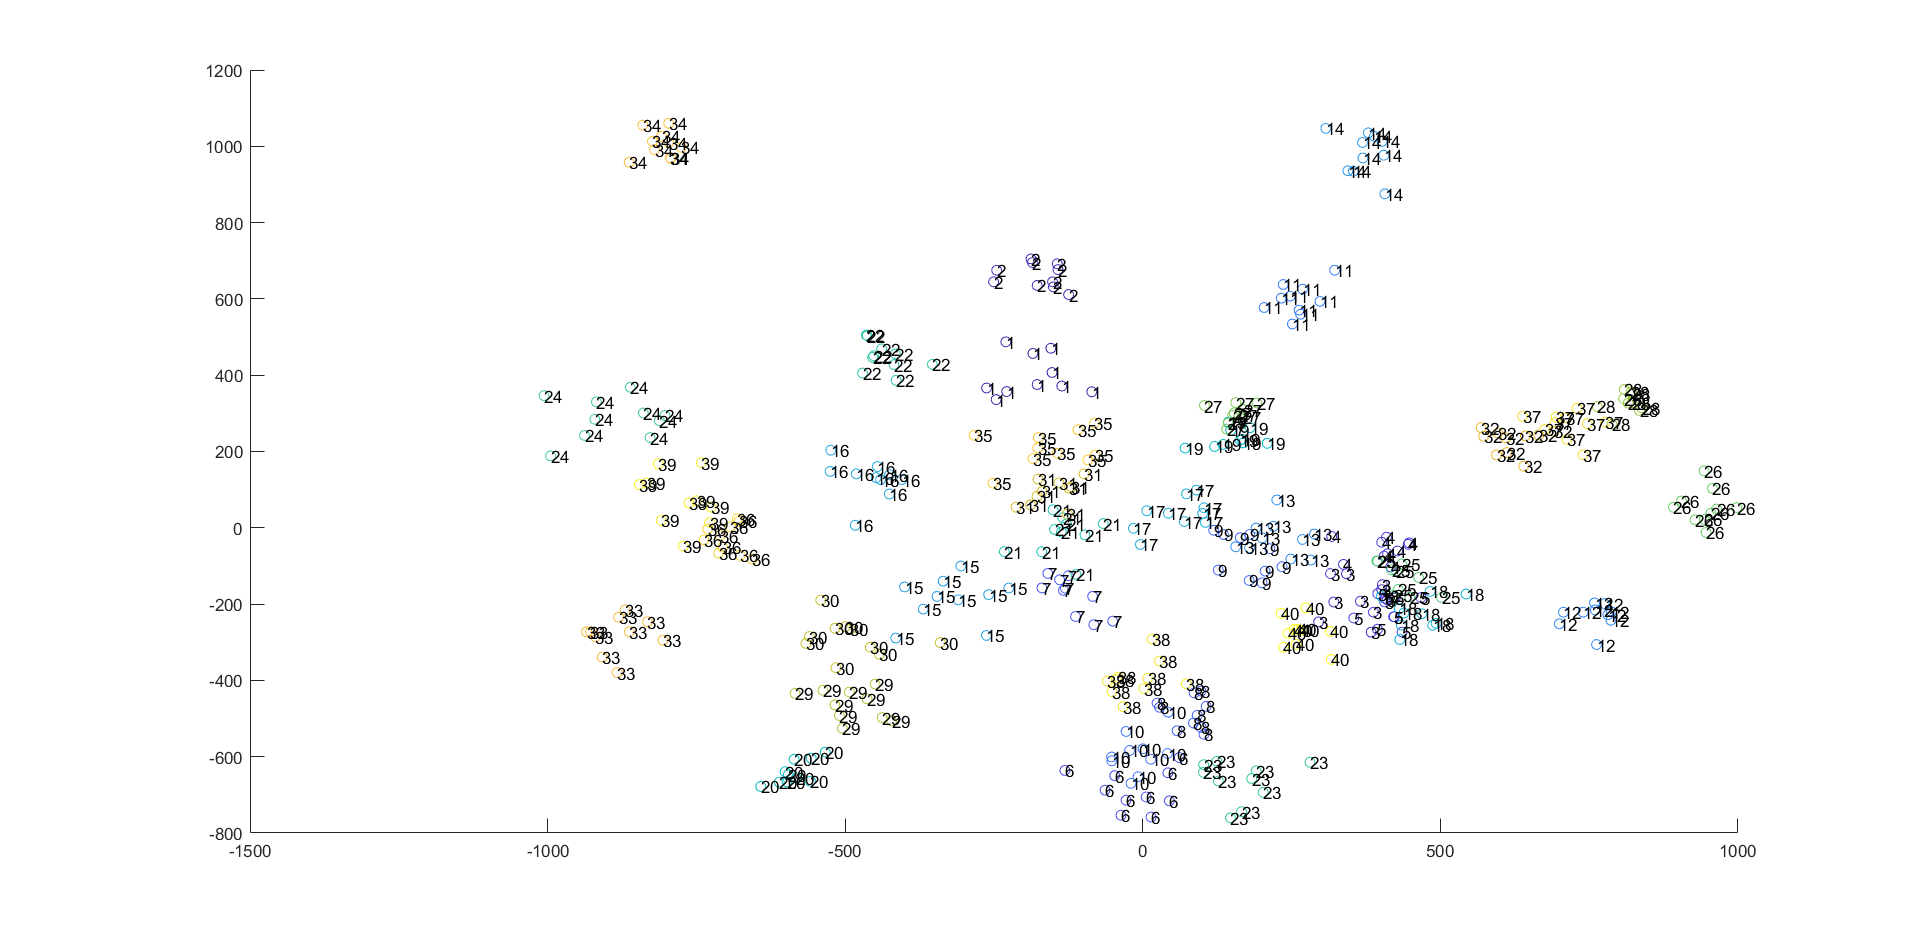
\includegraphics[width=\textwidth, height=\textheight, keepaspectratio]{fisherfaces.png}
\end{figure}

\section{Bag of words}
Questa metodologia di classificazione basa il suo funzionamento sul calcolo della \textit{frequenza} con cui un pattern si presenta all'interno di un documento di testo (bag of words) o di un'immagine (bag of visual words). L'idea di fondo è quella di \textit{individuare} degli elementi caratterizzanti da un dataset tramite procedure adatte al problema studiato (suddivisione tramite griglia, individuazione di punti di interesse, campionamento casuale, segmentazione basata su patches, algoritmo SIFT, ecc.).

Poi, tramite il \textit{dictionary learning} si costruiscono i clusters, ovvero dei gruppi naturali di campioni accomunati da un determinato insieme di pattern caratterizzanti. L'estrazione di queste patch permette di generare un dizionario di elementi avente la forma di un \textit{istogramma}. Nella fase di \textit{riconoscimento} ogni elemento viene confrontato con gli elementi estratti dal campione da classificare utilizzando un opportuno modello. Solitamente, il riconoscimento di oggetti incogniti avviene tramite approccio generativo (modelli grafici) o discriminativo
(Support Vector Machines, SVM).
\begin{figure}[htp]
	\centering
	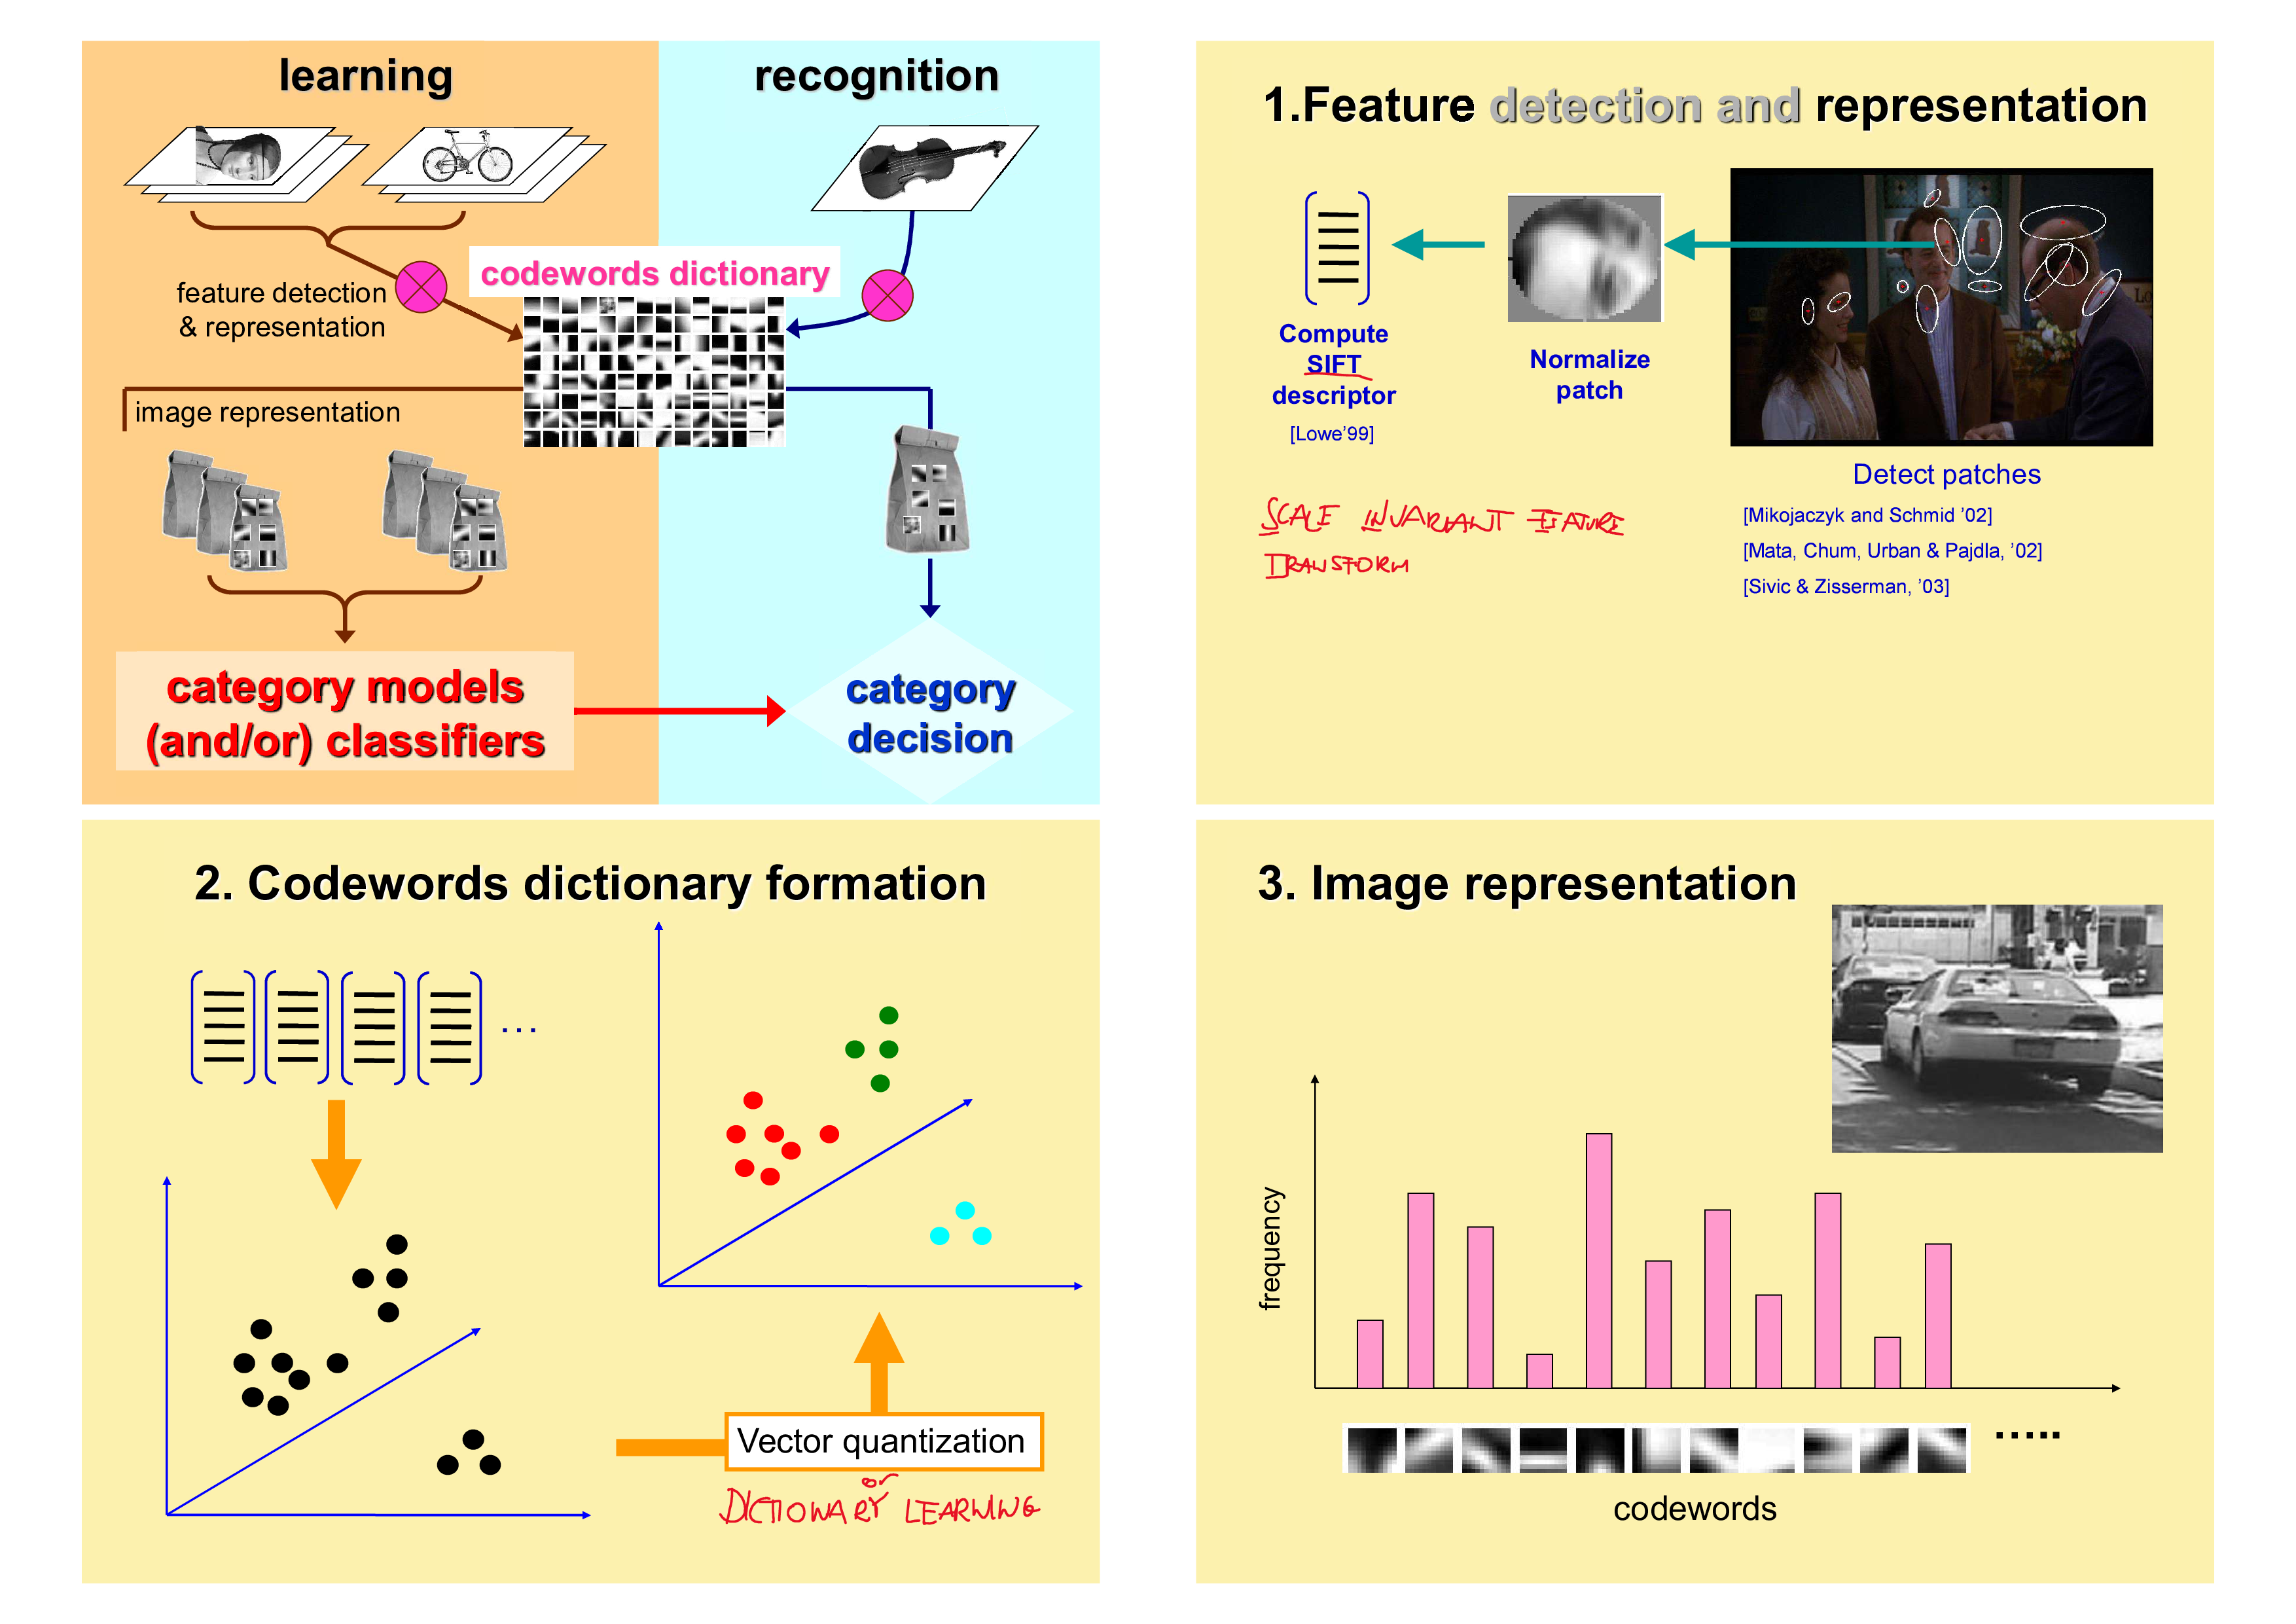
\includegraphics[width=\textwidth, height=\textheight, keepaspectratio]{bow.png}
\end{figure}


\chapter{Learning}

\section{Stima parametrica}
Lo scopo del \textit{learning} è quello di definire delle superfici nello spazio delle features che dividano le diverse classi. In particolare, nel learning \textit{parametrico} si vogliono stimare i parametri di una distribuzione i cui confini sono proprio le superfici. Un possibile approccio per la stima di questi parametri è chiamato maximum likelihood estimation.

\subsection{Approccio maximum likelihood (caso mono-modale)}
Per ipotesi, sappiamo che $\theta$ è un set di parametri fissato (ma sconosciuto) tale per cui dato un certo dataset $D$:
\[ p(D|\theta) = \prod_{k=1}^n p(x_k|\theta) \]
Tale funzione di $\theta$ è chiamata likelihood, per cui la stima della sua massimizzazione è detta, per definizione, \textit{maximum likelihood} di $\theta$ ed è rappresentata dal valore $\hat{\theta}$.
\begin{figure}[htp]
	\centering
	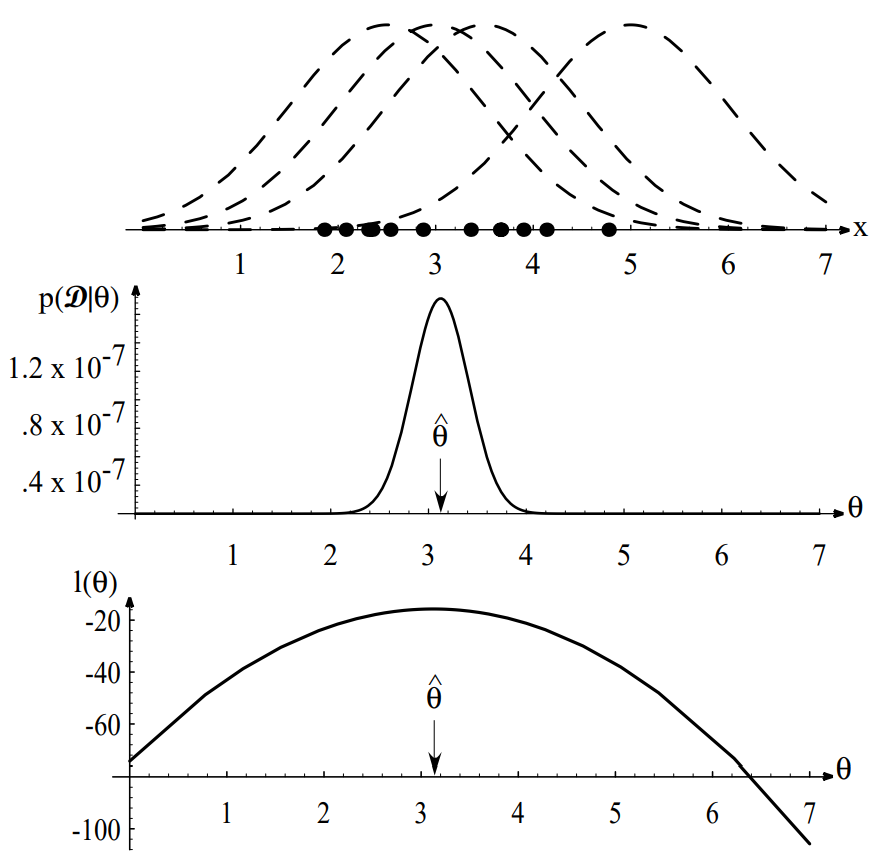
\includegraphics[width=0.5\textwidth]{ll.png}
\end{figure}

\noindent
Per scopi analitici, è preferibile scrivere la funzione di likelihood in forma logaritmica (vedi figura precedente). Per cui prima di tutto definiamo il gradiente di $\theta = (\theta_1,...,\theta_p)^t$ (in funzione del parametro $t$) come:
\[ \nabla_{\theta} \equiv \left[ \substack{\frac{\partial}{\partial \theta_1} \\ \dots \\ \frac{\partial}{\partial \theta_p}} \right] \]
La \textit{log-likelihood} sarà quindi espressa come:
\[ l(\theta) \equiv \ln p(D|\theta) = \sum_{k=1}^n \ln p(x_k|\theta) \]
A questo punto, per ottenere il set di parametri che massimizza $l(\theta)$, dovremo stimare:
\[ \argmax_{\theta} l(\theta) = \hat{\theta} \]
Per calcolare questo massimo, facciamo la derivata della log-likelihood
\[ \nabla_{\theta} l = \sum_{k=1}^n \nabla_{\theta} \ln p(x_k|\theta) \]
e la poniamo a zero per trovare i punti di minimo/massimo/flesso:
\[ \nabla_{\theta} l = 0 \]
Nel caso di \textit{distribuzioni multivariate} dovremo quindi stimare $\mu$ e $\Sigma$. Per semplicità, consideriamo solo $\mu$ e concentriamoci su un singolo dato $x_i$. Avremo:
\[ \ln p(x_i|\mu) = - \frac{1}{2} \ln [(2\pi)^d |\Sigma|] - \frac{1}{2} (x_i - \mu)^t \Sigma^{-1} (x_i - \mu) \]
Facendo la derivata passiamo a:
\[ \nabla_{\mu} \ln p(x_i|\mu) = \Sigma^{-1} (x_i - \mu) \]
Per calcolare il massimo poniamo la derivata a zero
\[ \Sigma^{-1} (x_i - \mu) = 0 \]
e troviamo che:
\[ \hat{\mu} = \frac{1}{n} \cdot \sum_{i=1}^n x_i \]

\subsection{Approccio maximum likelihood (caso multi-modale)}
Nel caso in cui la funzione di likelihood risulta particolarmente complessa (ad esempio è una \textit{mistura di Gaussiane}), non si è in grado di calcolarne la differenziabilità per trovare i punti di interesse.

Per una distribuzione multi-modale, i parametri da stimare saranno un certo insieme ripetuto per ciascuna moda. Si può quindi pensare che ciascuna moda potrebbe essere vista come una \textit{classe} e, secondo lo stesso principio, i parametri delle distribuzioni potrebbero essere visti come un classificatore.
\begin{figure}[htp]
	\begin{subfigure}{0.49\textwidth}
	    \centering
		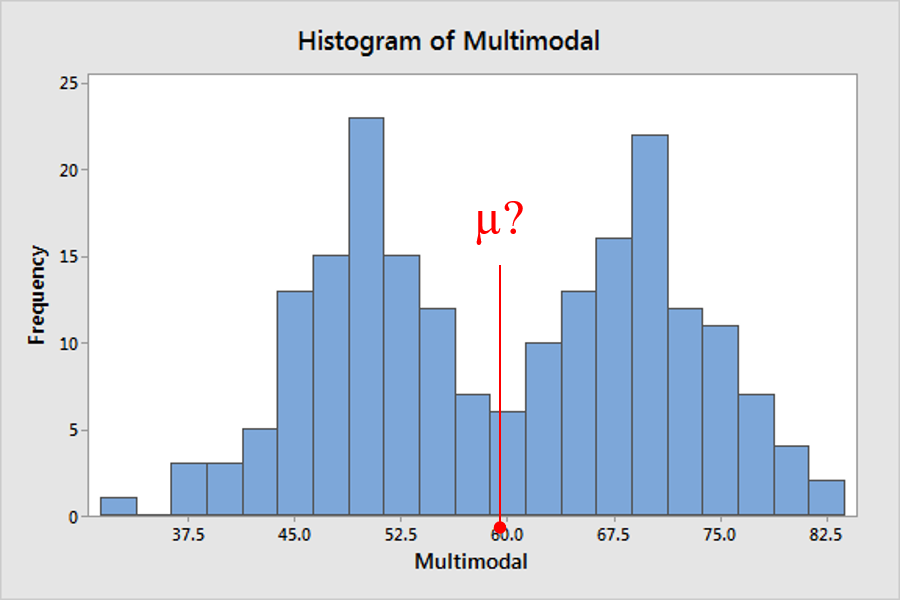
\includegraphics[width=\textwidth, height=\textheight, keepaspectratio]{multimodal1.png}
		\caption{Mistura di Gaussiane}
	\end{subfigure}
	\hfill
	\begin{subfigure}{0.49\textwidth}
	    \centering
		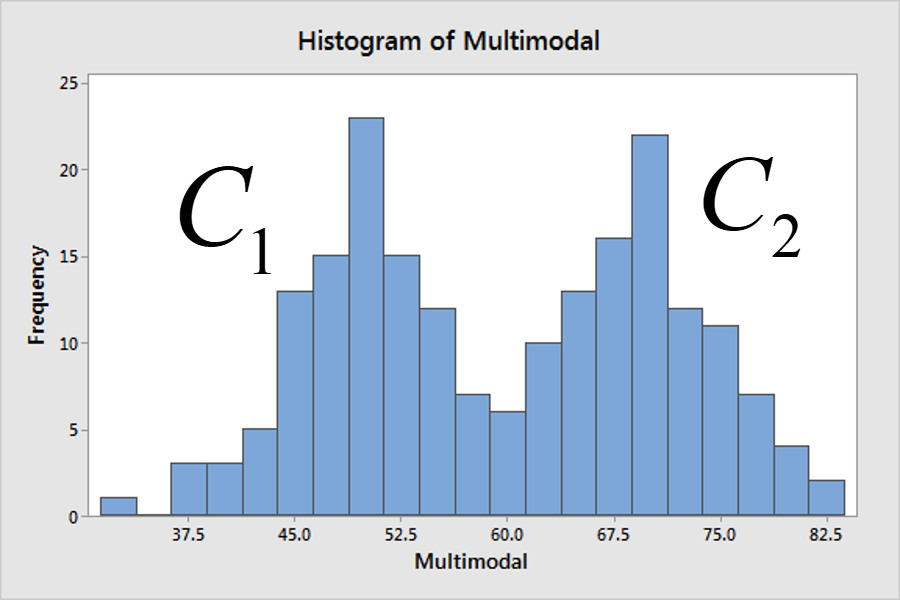
\includegraphics[width=\textwidth, height=\textheight, keepaspectratio]{multimodal2.png}
		\caption{Ogni moda è una classe}
	\end{subfigure}
\end{figure}

\noindent
L'assegnazione di ogni campione ad una moda può essere trovata applicando il teorema di Bayes:
\[ p(C_j|x_i) = \frac{p(x_i|C_j) \cdot p(C_j)}{p(x_i)} = \frac{p(x_i|C_j) \cdot p(C_j)}{\sum_j p(x_i|C_j) \cdot p(C_j)} \]
Per studiare la probabilità a posteriori dovremo stimare le probabilità a priori $p(C_j)$ e le funzioni di likelihood $p(x_i|C_j)$. Di solito, le probabilità a priori vengono fornite e perciò non è necessario stimarle:
\[ p(C_j) = \frac{n_j}{n} \]
dove $n_j$ è il numero di campioni con classe $C_i$.

Per stimare le funzioni di likelihood, invece, dobbiamo prima stimare il tipo di funzione $p(x_i|C_j)$ da utilizzare (Gaussiana, esponenziale, ecc.) e poi stimarne i parametri. Nel caso della Gaussiana, la distribuzione da stimare sarebbe:
\[ \sum_{j=1}^K \pi_j \cdot \mathcal{N}(\mu_j, \Sigma_j) \]
La stima di questa distribuzione è decisamente più difficile in quanto, dopo aver derivato per ogni singolo parametro, non si riesce ad ottenere un sistema lineare chiuso (ovvero non si riescono a disaccoppiare i parametri).

In questi casi si adotta un algoritmo ausiliario chiamato \textit{Expectation Maximization} (EM), il quale prende il nome dalle due fasi in cui si articola:
\begin{enumerate}
    \item Assumere di focalizzarsi su ogni moda della densità valutando $p(C_j|x_i)$ per ogni $j$ (fase di Expectation).
    \item Calcolare i parametri per ogni moda $C_j$ (fase di Maximization).
    \item Ripetere i punti 1 e 2 fino alla convergenza dei parametri.
\end{enumerate}

\subsection{K-means}
\label{K-means}
Prima di mostrare il funzionamento dell'algoritmo EM diamo uno sguardo a \textit{K-means}. Questo algoritmo è una variante più semplice di EM, in quanto stima solo la media $\mu_j$.
\newpage
\noindent
K-means può quindi essere visto come un algoritmo EM in cui le due fasi si mappano in:
\begin{enumerate}
    \item Calcolare $p(C_j|x_i)$ come la distanza euclidea $d$ di $x_i$ rispetto a $\mu_j$.
    \item Associare ogni $x_i$ alla classe $\tilde{C}_j$ per cui vale
    \[ \tilde{C}_j = \argmax_{C_j} p(C_j|x_i) = \argmin_{\mu_j} d(x_i,\mu_j) \]
    \item Ricalcolare $\mu_j$ per ogni $j$.
\end{enumerate}
A partire da una clusterizzazione iniziale (il numero di clusters deve essere fissato a priori), l'\textit{algoritmo} K-means assegna ad ogni iterazione tutti i pattern al cluster con la media più vicina e poi aggiorna le medie, terminando nel caso in cui sia giunto a convergenza. Questo algoritmo ha un'efficienza lineare nella dimensione del dataset, perciò risulta ottimo per grandi insiemi di dati.
\begin{figure}[htp]
	\begin{subfigure}{0.49\textwidth}
	    \centering
		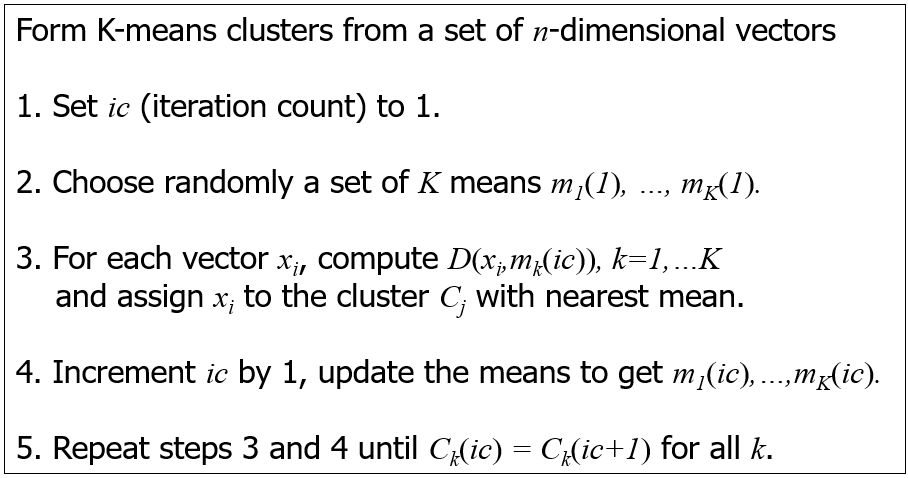
\includegraphics[width=\textwidth, height=\textheight, keepaspectratio]{k-means1.png}
		\caption{Algoritmo di clustering con K-means}
	\end{subfigure}
	\hfill
	\begin{subfigure}{0.49\textwidth}
	    \centering
		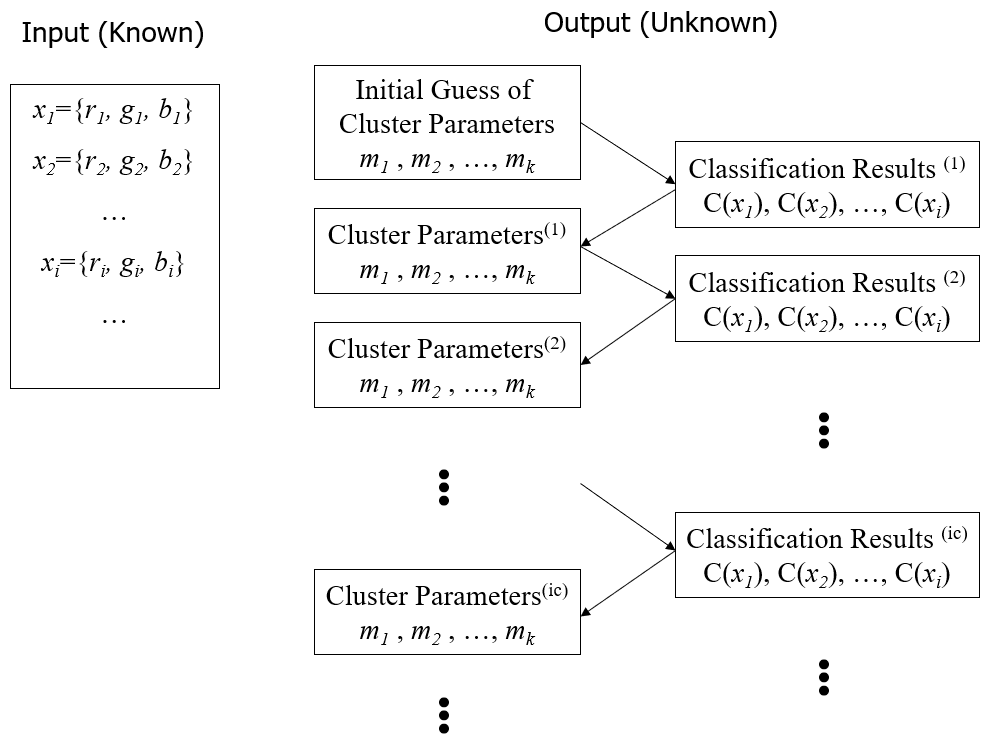
\includegraphics[width=\textwidth, height=\textheight, keepaspectratio]{k-means2.png}
		\caption{Classificatore K-means}
	\end{subfigure}
\end{figure}

\subsection{Algoritmo EM}
\label{EM}
L'\textit{algoritmo EM} tende a convergere ad un massimo locale adottando una procedura iterativa, che ha lo scopo di calcolare la maximum-likelihood, in cui si alternano due fasi:
\begin{enumerate}
    \item Quella di \textit{Expectation}, che crea una funzione di stima per la media della log-likelihood a partire dagli ultimi parametri stimati.
    \item Quella di \textit{Maximization}, che calcola i parametri che massimizzano tale funzione; questi ultimi verranno poi riutilizzati per eseguire la successiva fase di Expectation.
\end{enumerate}
Il caso tipico in cui si usa EM è quello in cui i dati sono distribuiti secondo una \textit{mistura di Gaussiane}. Infatti, EM analizza i dati che si sovrappongono e, col procedere delle iterazioni, identifica i valori massimi che corrispondono alle medie delle Gaussiane presenti nella mistura.
\begin{figure}[htp]
	\begin{subfigure}{0.49\textwidth}
	    \centering
		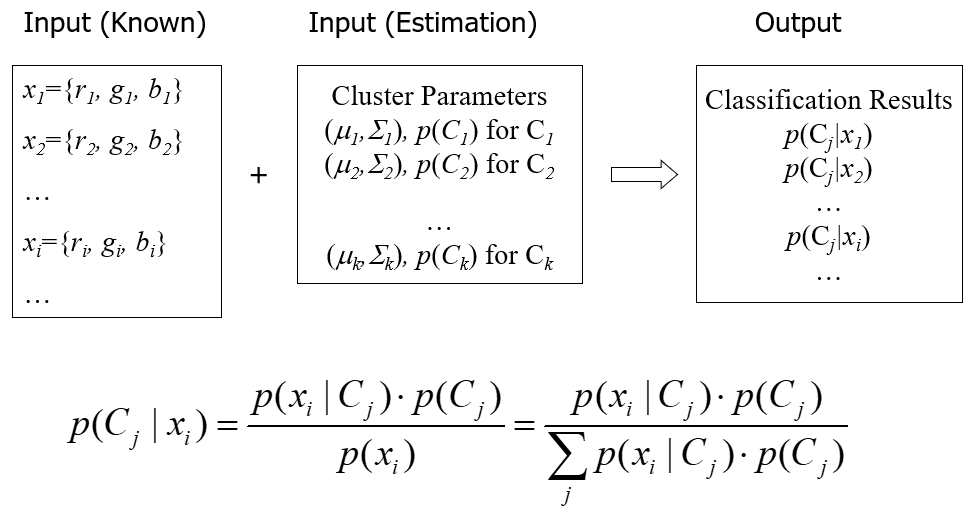
\includegraphics[width=\textwidth, height=\textheight, keepaspectratio]{em1.png}
		\caption{Fase di Expectation}
	\end{subfigure}
	\hfill
	\begin{subfigure}{0.49\textwidth}
	    \centering
		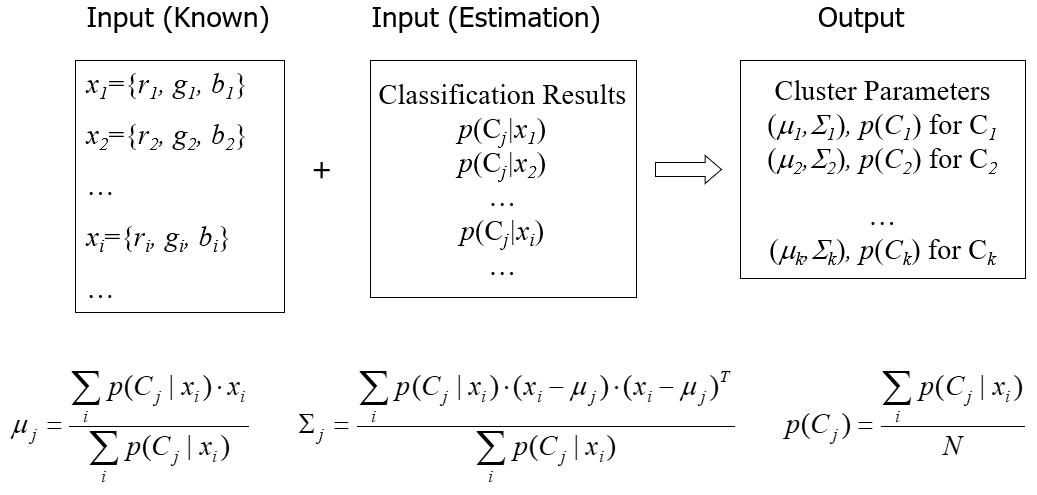
\includegraphics[width=\textwidth, height=\textheight, keepaspectratio]{em2.png}
		\caption{Fase di Maximization}
	\end{subfigure}
\end{figure}

\section{Stima non parametrica}
Nel \textit{learning non parametrico} non si fanno assunzioni sulla forma delle densità di probabilità, in quanto potrebbero essere sovra-strutturate. L'idea è quindi quella di studiare le regioni in cui si suddivide lo spazio. Infatti, se mi interessa studiare la probabilità $P(x|C)$, andrò ad osservare la regione $R$ dello spazio in cui l'oggetto è localizzato. Un problema di questo approccio consiste nella stima di $P(x|C) = P(x)$. I principali metodi utilizzabili per stimare $P(x)$ (per ogni possibile $x$) sono:
\begin{itemize}
    \item \textit{Parzen Windows}, in cui, fissata la regione $R$ centrata in $x$, si calcola la kernel function $K$ dai dati e si stima $P(x)$ (più punti sono presenti in $R$ e migliore sarà la stima).
    \item \textit{Meanshift}, in cui si cerca il centro di massa dei punti contenuti nella regione di interesse $R$ andando a calcolare il meanshift vector, il quale collega il centro della regione con il centro di massa appena calcolato (quest'ultimo diventerà poi il centro di $R$ al prossimo step).
\end{itemize}

\subsection{Parzen Windows}
Per ottenere la \textit{kernel function} $K$ (in forma analitica) ci affidiamo ad una window function che rappresenta la regione $R$ tale per cui, dato un punto $x_i$, se questo cade nella regione allora la funzione ritorna 1, altrimenti ritorna 0. Grazie a ciò, il metodo Parzen Windows riesce a garantire una serie di vantaggi:
\begin{itemize}
    \item Permette più tipi di window functions.
    \item Siccome la stima della PDF è data dalla media della window function su $x$ e $x_i$, ogni campione contribuisce, a seconda della distanza dalla media $x$, alla forma della PDF.
\end{itemize}
La formula finale della probabilità che un punto $x$ si trovi in una determinata regione $R$ è data quindi da:
\[ P(x) = \frac{1}{n} \cdot \sum_{i=1}^n K(x-x_i) \]
\newpage
\noindent
Per riuscire a fornire una buona approssimazione, la funzione $K$ deve avere le seguenti proprietà:
\begin{itemize}
    \item $K(x-x_i)$ deve essere maggiore o uguale a 0.
    \item $\argmax_x K(x-x_i) = x_i$ si deve avere per $x_i$ uguale alla media $x$.
    \item Deve essere simmetrica, ovvero $K(x-x_i) = K(-x+x_i)$.
    \item Deve essere normalizzata, ovvero $\int K(x-x_i) \, dx = 1$.
\end{itemize}
In Parzen Windows la scelta della \textit{bandwidth} è cruciale: se è troppo grande, si avrà una PDF poco informativa; se è troppo piccola, si otterrà una distribuzione di picchi localizzati sui punti stessi.
\begin{figure}[htp]
	\begin{subfigure}{0.49\textwidth}
	    \centering
		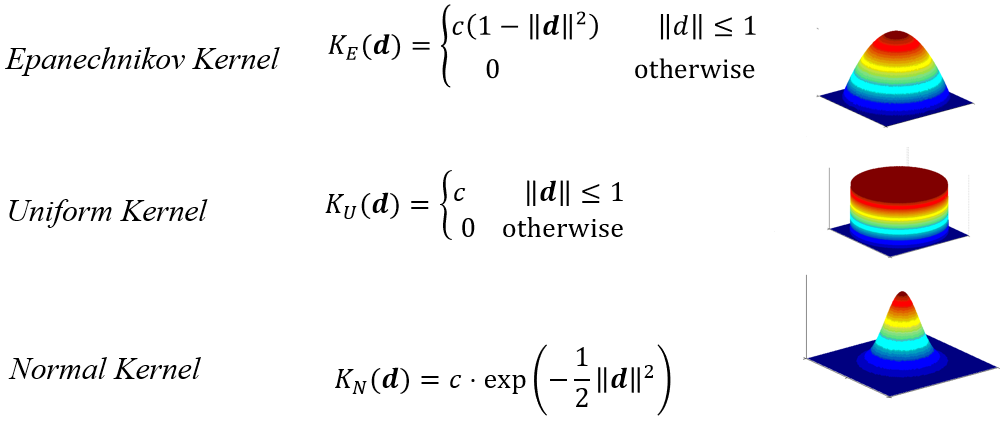
\includegraphics[width=\textwidth, height=\textheight, keepaspectratio]{pw1.png}
		\caption{Vari tipi di window functions}
	\end{subfigure}
	\hfill
	\begin{subfigure}{0.49\textwidth}
	    \centering
		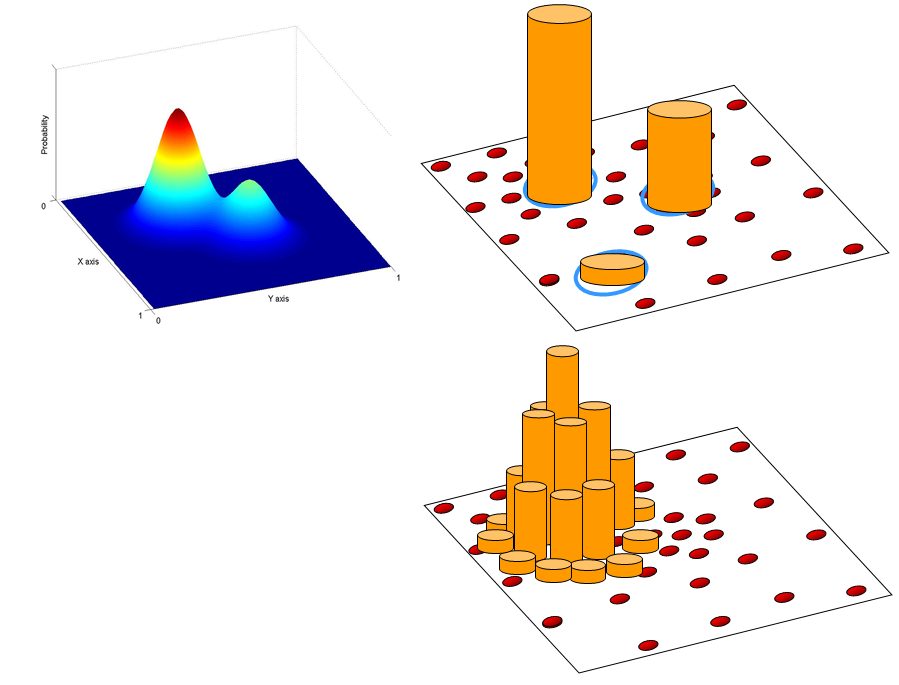
\includegraphics[width=\textwidth, height=\textheight, keepaspectratio]{pw2.png}
		\caption{Due esempi di scelta della bandwidth}
	\end{subfigure}
\end{figure}

\subsection{Meanshift}
Meanshift è una tecnica per la ricerca della regione (locale) più densa in un set di punti conosciuto. Questa tecnica evidenzia quindi la forma di una PDF in uno spazio $d$-dimensionale (dimensionalità di $R$). Le caratteristiche rappresentate possono essere di tipo posizionale, colorimetrico o altro.

La stima della densità dei punti nella regione studiata è detta \textit{kernel density estimation}, in quanto la densità dei punti in $R$ è calcolata sulla base di una funzione kernel $K$.
\begin{figure}[htp]
	\begin{subfigure}{0.49\textwidth}
	    \centering
		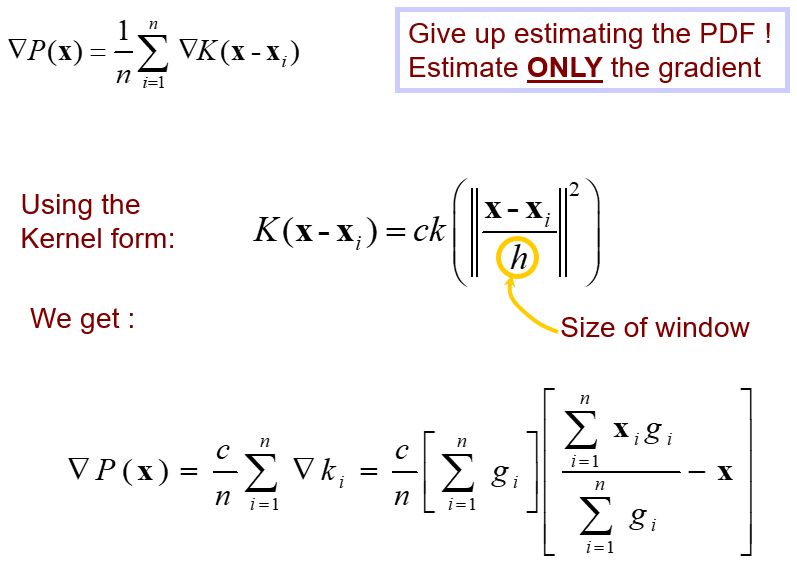
\includegraphics[width=\textwidth, height=\textheight, keepaspectratio]{ms1.png}
		\caption{Kernel density estimation}
	\end{subfigure}
	\hfill
	\begin{subfigure}{0.49\textwidth}
	    \centering
		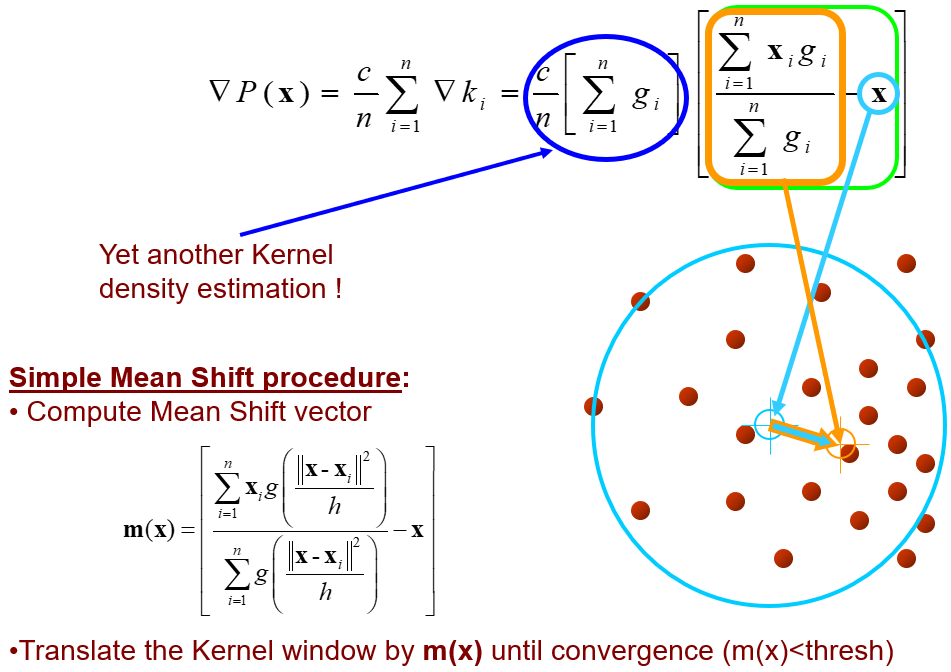
\includegraphics[width=\textwidth, height=\textheight, keepaspectratio]{ms2.png}
		\caption{Calcolo del meanshift vector}
	\end{subfigure}
\end{figure}
\newpage
\noindent
Siccome meanshift lavora con il gradiente del kernel, è possibile incappare in casi limite. \`{E} quindi più giusto parlare del meanshift come una tecnica non parametrica di stima del gradiente di densità. Le \textit{proprietà} garantite da questo approccio sono:
\begin{itemize}
    \item \textit{Velocità di convergenza automatica}, ossia il meanshift vector varia (in modulo) automaticamente in quanto meanshift è una tecnica di ascesa del gradiente adattiva.
    \item \textit{Infinitamente convergente}, ossia la convergenza è garantita solo per step infinitesimali (solitamente si pone una soglia alla lunghezza del meanshift vector).
    \item Un \textit{kernel uniforme} garantisce la convergenza in un numero finito di passi.
    \item Un \textit{kernel gaussiano} ritorna una traiettoria più smooth ma impiega più tempo rispetto a quello uniforme.
\end{itemize}
Inoltre, i \textit{vantaggi} di meanshift sono che:
\begin{itemize}
    \item \`{E} indipendente rispetto all'applicazione che si sta realizzando.
    \item \`{E} adatto per l'analisi di dati reali.
    \item Non necessita di assunzioni a priori sulla forma della distribuzione dei dati.
    \item Può gestire spazi delle features arbitrari.
    \item Richiede di scegliere un solo parametro, ossia la dimensione della finestra.
\end{itemize}
Infine il \textit{lato negativo}, che è proprio scegliere la dimensione della finestra, in quanto una scelta non felice potrebbe provocare un'errata ricerca del centro di massa. Una metodologia che consente di risolvere questo problema consiste nell'adattare la dimensione della finestra in base allo stato in cui ci si trova.
\begin{figure}[htp]
	\begin{subfigure}{0.49\textwidth}
	    \centering
		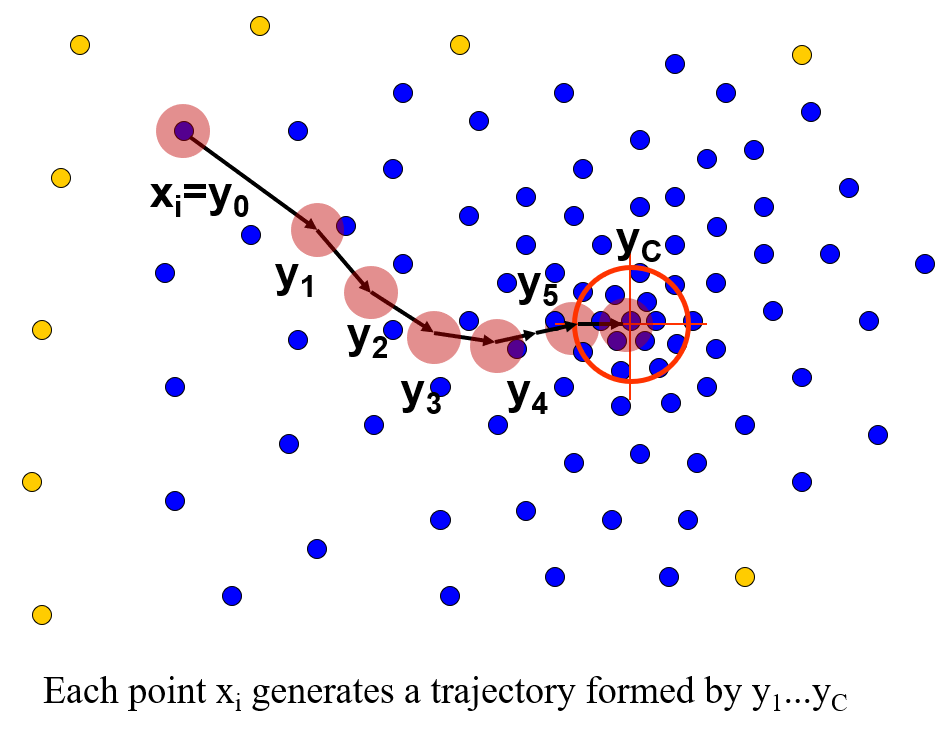
\includegraphics[width=\textwidth, height=\textheight, keepaspectratio]{ms3.png}
		\caption{Ricerca del centro di massa}
	\end{subfigure}
	\hfill
	\begin{subfigure}{0.49\textwidth}
	    \centering
		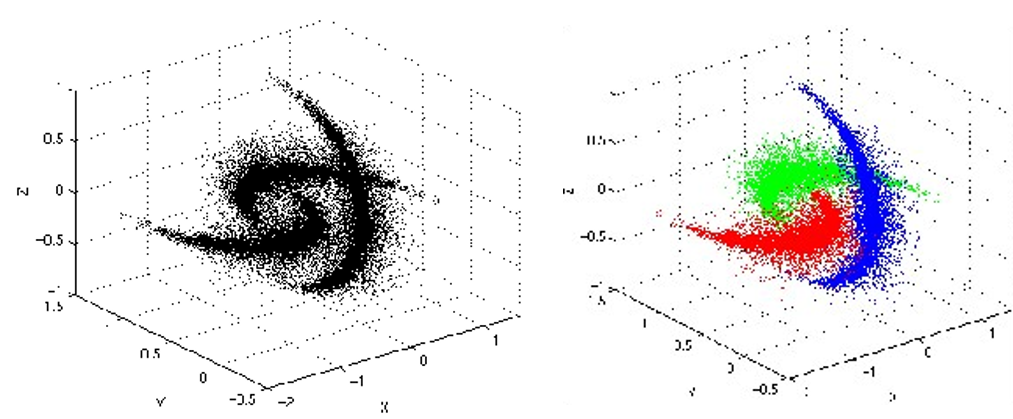
\includegraphics[width=\textwidth, height=\textheight, keepaspectratio]{ms4.png}
		\caption{PDF evidenziate}
	\end{subfigure}
\end{figure}

\subsection{Clustering con meanshift}
Normalmente, meanshift si applica tassellando lo spazio con una serie di finestre e lanciando una procedura in parallelo per evidenziare tante traiettorie quante sono le finestre. Ogni finestra tende a seguire la direzione di convergenza più veloce, ovvero ogni finestra ricerca il centro di massa più vicino (massimo locale della PDF). Questa peculiarità garantisce, in base al numero di procedure lanciate in parallelo, un uso ottimale in uno studio legato al \textit{clustering} dei dati. Infatti, la divisione in clusters avverrà considerando le traiettorie identificate dalle varie procedure.

Meanshift preserva le discontinuità. Nel caso delle immagini, quindi, viene lanciata per ogni pixel una procedura di meanshift (in cui la funzione kernel è pesata in funzione delle coordinate spaziali e colorimetriche) la quale arriverà ad una certa moda (centro di massa locale). Si assegna poi al pixel di partenza il valore (colore) della moda trovata. Ne consegue che meanshift permette la \textit{segmentazione delle immagini}, mantenendo le discontinuità e applicando una procedura di smoothing (ogni pixel assume il valore della moda a cui è collegato).
\begin{figure}[htp]
	\begin{subfigure}{0.49\textwidth}
	    \centering
		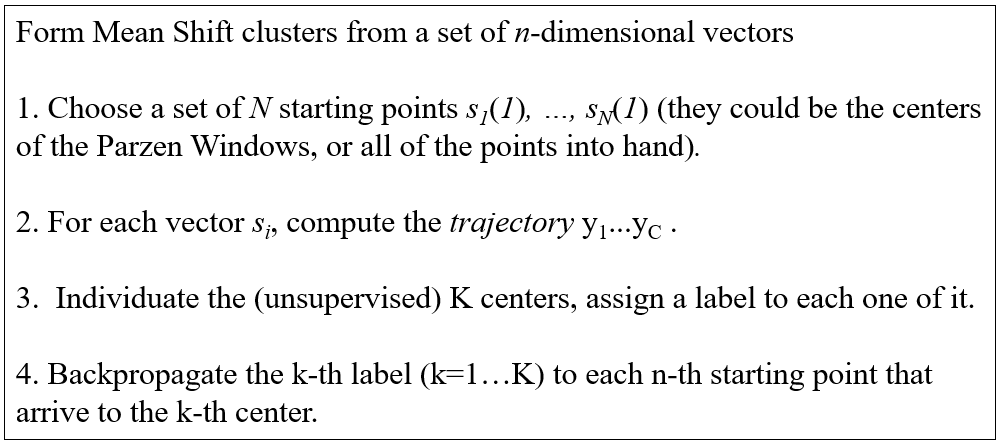
\includegraphics[width=\textwidth, height=\textheight, keepaspectratio]{clustering1.png}
		\caption{Algoritmo}
	\end{subfigure}
	\hfill
	\begin{subfigure}{0.49\textwidth}
	    \centering
		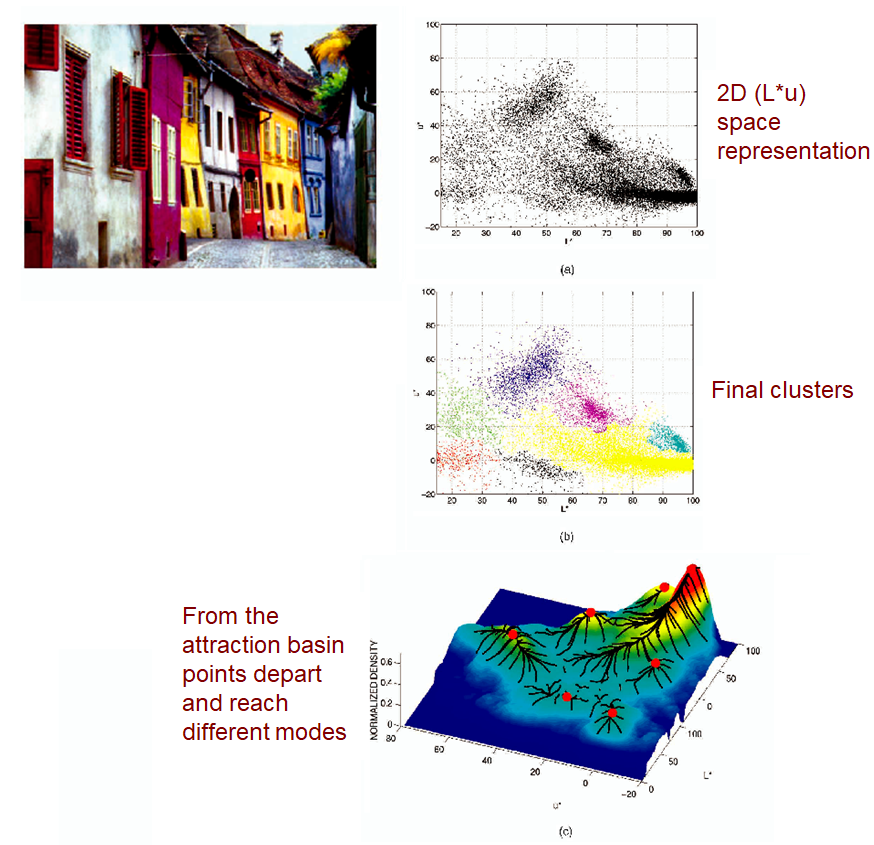
\includegraphics[width=\textwidth, height=\textheight, keepaspectratio]{clustering2.png}
		\caption{Clustering su immagini}
	\end{subfigure}
\end{figure}

\section{Tracking (stima di densità dinamiche)}
Lo scopo del \textit{tracking} è quello di capire dove si spostano gli oggetti in una sequenza, stimandone così la traiettoria. Le operazioni di tracking si articolano in una prima fase di \textit{inizializzazione}, dove si identificano i nuovi oggetti che entrano in scena (lo scopo è trovare un oggetto da seguire), e in una fase di \textit{inseguimento}, dove si vuole mantenere l'attenzione sui soggetti (lo scopo è riconoscerne l'identità). Gli approcci alla fase di inseguimento sono di due tipi:
\begin{itemize}
    \item Metodologia forza bruta, in cui si sfrutta la correlazione e la definizione di vincoli.
    \item Metodologia classica, in cui si fa predizione, verifica e associazione dei valori calcolati.
\end{itemize}
Tra le tecniche adottate nella fase di inizializzazione, invece, ci sono il template matching (con l'output di un classificatore come face detector o hand detector), la sottrazione del background e alcuni metodi ibridi.

\subsection{Inseguimento}
La fase di inseguimento vuole mantenere l'identità degli oggetti identificati, così da poterne tracciare e stimare la traiettoria di movimento. Il problema è trovare un metodo che permetta di associare gli oggetti identificati in un dato frame con quelli del frame successivo. Il metodo di forza bruta, basato sulla ricerca esaustiva dei singoli oggetti, risulta lento e impreciso. L'aggiunta di vincoli sulla scena e sulla natura degli oggetti, invece, permette una stima della posizione dei soggetti, pesando di conseguenza la correlazione in modo opportuno. Le tecniche di \textit{particle filtering} come il condensation (o metodo di Montecarlo) sono attualmente i metodi di stima più adottati.

\subsection{Particle filtering}
L'approccio tramite particle filtering parte da diverse \textit{assunzioni}:
\begin{itemize}
    \item Lo stato del sistema studiato all'istante di tempo $t$ è definito dalla posizione degli $M$ punti $X_t = \{ x_{1,t}, x_{2,t}, ..., x_{M,t} \}$.
    \item La storia (discreta) del sistema fino al tempo $t$, che indica un'evoluzione del sistema nel tempo, è definita come $\mathcal{X}_t = \{ X_1, X_2, ..., X_t \}$.
    \item Lo stato del sistema fino al tempo $t$ è osservabile da un set di osservazioni (immagini/frame) $\mathcal{Z}_t = \{ Z_1, Z_2, ..., Z_t \}$.
    \item Le osservazioni (vedi punto precedente) non modificano lo stato del sistema
    \[ p(\mathcal{Z}_{t-1}, X_t | \mathcal{X}_{t-1}) = p(X_t | \mathcal{X}_{t-1}) \cdot \prod_{i=1}^{t-1} p(Z_i | X_i) \]
    e sono indipendenti fra loro
    \[ p(\mathcal{Z}_t | \mathcal{X}_t) = \prod_{i=1}^t p(Z_i | X_i) \]
    \item L'evoluzione del sistema è considerato un processo stocastico Markoviano tempo-indipendente di ordine 1 $P(X_t | \mathcal{X}_t) = P(X_t | X_{t-1})$.
\end{itemize}
Quindi, l'\textit{obiettivo} del particle filtering è quello di stimare lo stato più probabile (atteso) del sistema $X_t$ date tutte le osservazioni $\mathcal{Z}_t$. Per fare questo, è necessario studiare la seguente probabilità (in forma Bayesiana):
\[ p(X_t | \mathcal{Z}_t) = k_t \cdot p(Z_t | X_t) \cdot p(X_t | \mathcal{Z}_{t-1}) \]
dove
\[ p(X_t | \mathcal{Z}_{t-1}) = \int_{X_{t-1}} p(X_t | X_{t-1}) \cdot p(X_{t-1} | \mathcal{Z}_{t-1}) \, dX_{t-1} \]
Il controllo ad ogni istante di tempo per questa probabilità corrisponde alla valutazione dell'evoluzione di una distribuzione nel tempo.

\subsection{Algoritmo di Condensation}
L'algoritmo di Condensation è una tecnica di particle filtering che si basa sul concetto di localizzazione spaziale dello stato del sistema. Assumendo di poter rappresentare in uno spazio (campo di esistenza $R$) finito e monodimensionale lo stato del sistema, si può affermare che lo stato è rappresentabile come un punto su $R$ e quindi che il sistema è
una particella puntiforme su tale campo di esistenza.

La fase di \textit{inizializzazione} prevede che siano dati $N$ campioni (particelle su $R$) che rappresentano i possibili stati del mio sistema ad un certo istante $t-1$; tale set di particelle è definito come:
\[ \{ s_{t-1}^{(n)} \} \]
All'istante iniziale si settano i pesi per tutte le particelle (ogni campione rappresenta un intorno spaziale locale); tale set di pesi è definito come:
\[ \{ \pi_{t-1}^{(n)} \} \]
L'assegnazione dei pesi alle particelle permette di stimare una PDF su tutto $R$.

Finita l'inizializzazione inizia la fase di \textit{tracking}, in cui il particle filtering fa evolvere il set di particelle in tre passi.
\begin{enumerate}
    \item \textit{Selezione o campionamento}: a partire dalla PDF al tempo $t-1$, estraggo $N$ nuove particelle (ogni particella ha probabilità di estrazione pari al suo peso).
    \item \textit{Applicazione della dinamica}: ad ognuna delle nuove particelle applico un moto con una componente deterministica (basata sul passo precedente) e una probabilistica aggiungendo del rumore gaussiano per modellare l'incertezza sul moto; questo permette di calcolare la parte predittiva (a priori) $p(X_t | \mathcal{Z}_{t-1})$ della formulazione Bayesiana del filtro.
    \item \textit{Valutazione/pesatura}: a partire dalle osservazioni, calcolo la likelihood di ogni campione.
\end{enumerate}
Con la nuova PDF calcolata si associano i pesi (normalizzati) alle nuove particelle. A questo punto basta prendere una \textit{decisione} sulla posizione del soggetto ad un certo istante $t$, ad esempio si può effettuare un calcolo basato sulla media pesata oppure tramite MAP (Maximum A Posteriori).
\begin{figure}[htp]
	\begin{subfigure}{0.49\textwidth}
	    \centering
		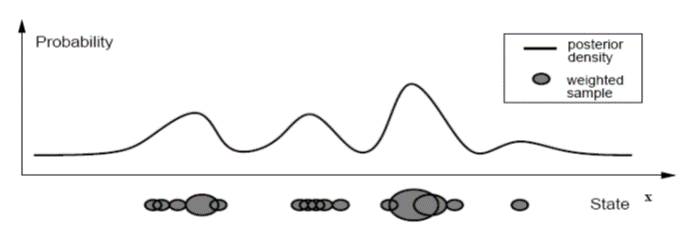
\includegraphics[width=\textwidth, height=\textheight, keepaspectratio]{condensation1.png}
		\caption{Inizializzazione (PDF stimata)}
	\end{subfigure}
	\hfill
	\begin{subfigure}{0.49\textwidth}
	    \centering
		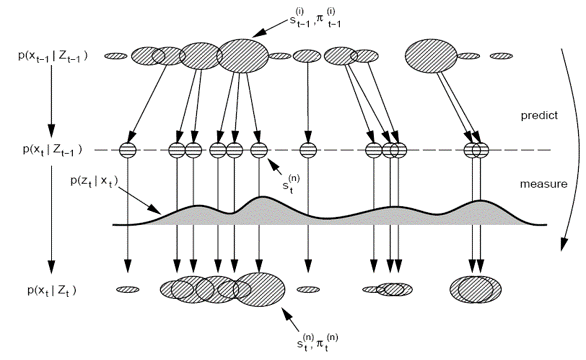
\includegraphics[width=\textwidth, height=\textheight, keepaspectratio]{condensation2.png}
		\caption{Tracking}
	\end{subfigure}
\end{figure}
\newpage

\subsection{Campionamento delle particelle}
Uno dei problemi da affrontare è il metodo di \textit{campionamento} delle particelle. Presi tutti i pesi dei campioni, ne faccio la somma cumulativa, ottenendo così una serie di coefficienti
\[ \{ c_t^{(n)} \} \]
Questo permette di effettuare i calcoli in modo efficiente (complessità pari a $O(N \log N)$). Infatti, generato casualmente un valore intero $r \in [0,1]$, si cerca per divisione binaria il più piccolo indice $j$ tale per cui
\[ c_{t-1}^{(j)} \geq r \]
e infine si setta
\[ s_t^{'(n)} = s_{t-1}^{(j)} \]

\subsection{Multi-object tracking}
Per quel che riguarda il tracking, l'algoritmo di Condensation tende effettivamente a seguire un unico oggetto. Quindi la robustezza di questa fase è vincolata alla stima della \textit{dinamica}, che tipicamente è fatta off-line (via correlazione esaustiva o manualmente) così da averla il più precisa possibile.

Il \textit{metodo Bramble} (Bayesian Multiple-BLob) è un metodo di tracking che può essere considerato come l'evoluzione del Condensation (Condensation multi-oggetto). L'idea consiste, come per il Condensation, di esprimere la probabilità di stato in funzione delle osservazioni. Tuttavia, lo stato del sistema non è più costituito solo dalle posizioni degli oggetti ma da una serie di parametri, ovvero il numero di oggetti e lo stato degli oggetti: $X_t = (m, x_t^1, ..., x_t^m)$. Ogni oggetto è poi una struttura di parametri $x=(i,l,v,s)$ dove:
\begin{itemize}
    \item $i$ è l'identità, ossia un indice identificativo.
    \item $l$ è la posizione (locazione), ossia le coordinate spaziali.
    \item $v$ è la velocità (espressa come vettore).
    \item $s$ è l'aspetto, ossia un fattore legato all'occlusione.
\end{itemize}
Lo stato del sistema $X_t$ è approssimato con un set di $N$ particelle (configurazioni):
\[ \{ S_t^{(n)}, \pi_t^{(n)} \} \]
Le osservazioni prevedono un campionamento delle immagini (frame) sufficiente a poter valutare il filtraggio in tempo reale. Ogni cella (o filtro) corrisponde ad una determinata posizione spaziale che avrà di conseguenza una particolare probabilità di successo (peso).
\begin{figure}[htp]
	\centering
	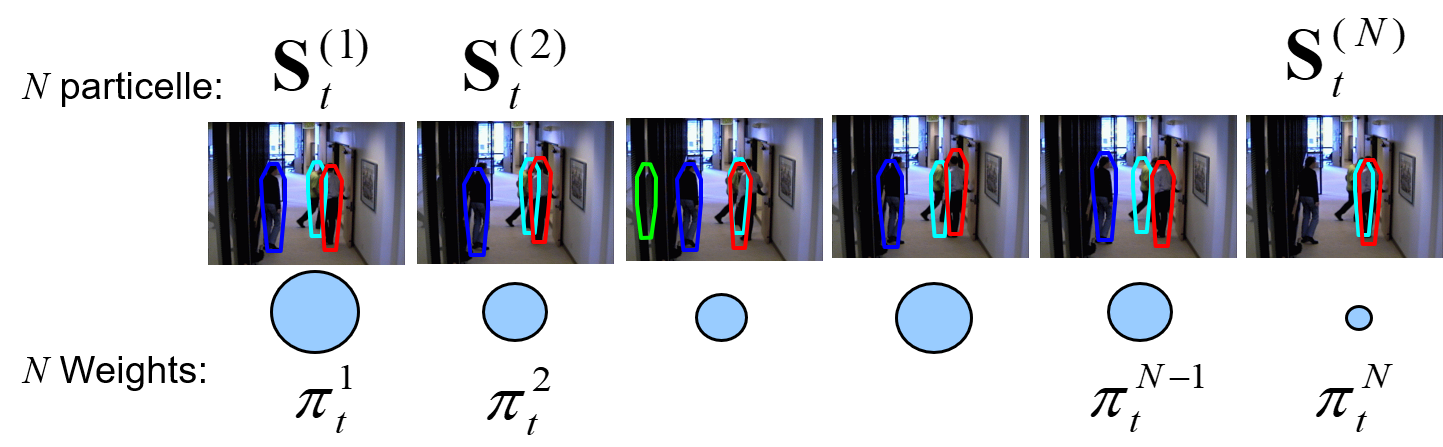
\includegraphics[width=0.65\textwidth]{bramble.png}
\end{figure}


\chapter{Classificatori generativi}

\section{Processi di Markov}
Un \textit{processo di Markov} è costituito da $N$ stati $s_1, ..., s_N$ ed è caratterizzato da un certo numero di passi discreti. La probabilità di partire da un determinato stato è dettata dalla distribuzione $\Pi = \{ \pi_i \}: \, \pi_i = P(q_1=s_i)$ dove $1 \leq i \leq N$, $\pi_i \geq 0$ e $\sum_{i=1}^N \pi_i=1$.

Al $t$-esimo istante il processo si trova esattamente in uno degli stati a disposizione, indicato dalla variabile $q_t$. Ad ogni iterazione, lo stato successivo viene scelto con una certa probabilità. Tale probabilità è unicamente determinata dallo stato precedente; per questo si parla di Markovianità del primo ordine.
\[ P(q_{t+1}=s_j | q_t=s_i, q_{t-1}=s_k, ..., q_1=s_l) = P(q_{t+1}=s_j | q_t=s_i) \]
Per descrivere un processo Markoviano si costruisce la matrice $A$ detta di transizione tra stati (invariante nel tempo), la quale è una matrice $N \times N$ in cui ogni elemento è definito come $a_{i,j} = P(q_{t+1}=s_j | q_t = s_i)$. Quindi, i processi Markoviani (discreti) sono caratterizzati da:
\begin{itemize}
    \item Markovianità del primo ordine.
    \item Stazionarietà.
    \item Avere una distribuzione iniziale.
\end{itemize}

\subsection{Modelli di Markov}
Conoscendo le caratteristiche dei processi di Markov è possibile esibire un modello probabilistico di Markov (MM), definito come $\lambda = (A, \pi)$. Un \textit{modello di Markov} è un modello stocastico che permette di descrivere tramite probabilità le cause che portano da uno stato all'altro del sistema, definendo così delle relazioni (probabilistiche) di causa-effetto tra gli stati. Su questo tipo di modelli si possono effettuare operazioni di \textit{training} (costruendo gli elementi costituenti del modello) e operazioni di \textit{interrogazione} (come per esempio richiedere la probabilità di avere una certa sequenza di stati).
\newpage
I modelli di Markov modellano comportamenti stocastici Markoviani (di ordine $N$) di un sistema in cui gli stati sono:
\begin{itemize}
    \item \textit{Espliciti}, ovvero riesco a dar loro un nome.
    \item \textit{Osservabili}, ovvero ho delle osservazioni che identificano univocamente lo stato.
\end{itemize}
Per esempio, in un sistema \textit{semaforo} gli stati sono tre e sono espliciti (lampade accese/spente) e osservabili (colori delle lampade). Inoltre, ogni stato ha la stessa probabilità iniziale e la matrice di transizione $A$ definisce le probabilità di passare da rosso a verde, da rosso a giallo, da verde a giallo, e così via.
\begin{figure}[htp]
	\centering
	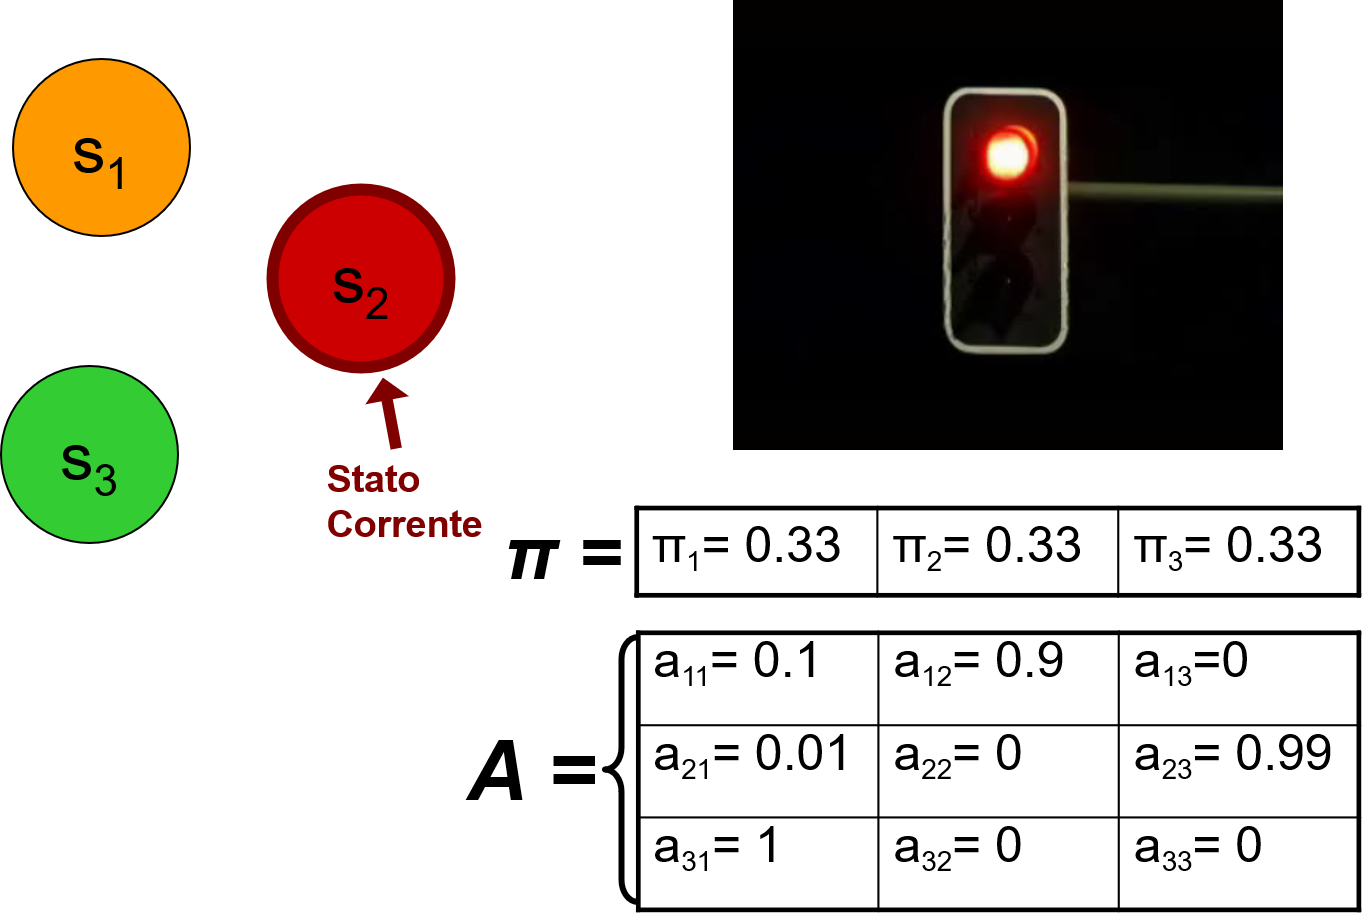
\includegraphics[width=\textwidth, height=\textheight, keepaspectratio]{semaforo.png}
\end{figure}

\subsection{Inferenze}
Per definire le relazioni probabilistiche dell'evoluzione di un modello di Markov (ovvero di una sequenza di stati da $q_1$ a $q_t$) possiamo scrivere:
\[ P(q_t,...,q_1) = P(q_t|q_{t-1}) P(q_{t-1}|q_{t-2}) ... P(q_2|q_1) P(q_1) \]
Inoltre, il calcolo della probabilità di trovarsi in un determinato stato in un certo istante di tempo è $P(q_t=s_j)$. La sua valutazione si articola in due step:
\begin{enumerate}
    \item Valuto come calcolare $P(Q)$ per ogni cammino di stati $Q = \{ q_1, q_2, ..., q_t=s_j \}$, ossia $P(q_t, q_{t-1}, ... q_1)$.
    \item Calcolo $P(q_t=s_j) = \sum_Q P(Q)$ dove con $Q$ si indicano tutti i cammini di lunghezza $t$ che finiscono in $s_j$.
\end{enumerate}
Questa valutazione risulta tuttavia molto onerosa (complessità pari a $O(N^t)$).

L'idea è quindi quella di riscrivere la probabilità $P(q_t=s_j)$ come $p_t(j)$, da cui possiamo definire induttivamente
\[ \forall i \, p_1(i) =
    \begin{cases}
	\pi_i & \text{se $s_i$ è lo stato in cui mi trovo} \\
	0 & \text{altrimenti}
	\end{cases} \]
\[ \forall j \, p_{t+1}(j) = P(q_{t+1}=s_j) = \sum_{i=1}^N P(q_{t+1}=s_j, q_t=s_i) \]
e ottenere
\[ \sum_{i=1}^N P(q_{t+1}=s_j | q_t=s_i) \cdot P(q_t=s_i) = \sum_{i=1}^N a_{ij} \cdot p_t(i) \]
Se si usa questo metodo partendo da $P(q_t=s_j)$ e procedendo a ritroso, il costo della computazione diventa $O(tN^2)$.

\subsection{Limiti dei modelli Markoviani}
Un limite dei modelli Markoviani è la necessità di avere stati \textit{osservabili deterministicamente}, e questo non sempre è possibile. Se ho un sistema dove ci sono stati non espliciti posso tuttavia studiarne la natura osservandone l'\textit{evoluzione}. A questo punto non conosco ancora quali siano gli stati regolatori, ma posso determinarne il
numero (e la categoria) \textit{osservando} il sistema (introduco una conoscenza a priori). A partire dalle osservazioni stabilisco poi una relazione tra osservazione e stato nascosto.

\section{Hidden Markov Models}
Tra i principali modelli generativi troviamo i modelli Markoviani a stati nascosti (HMM). Gli \textit{HMM} hanno lo scopo di descrivere probabilisticamente la dinamica di un sistema tralasciando la definizione delle cause che ne regolano l'evoluzione. Gli stati vengono quindi identificati solo tramite le osservazioni e in maniera probabilistica. In sostanza, gli HMM possono essere considerati come un'estensione dei modelli di Markov, in cui l'unica differenza sta nella non osservabilità degli stati. Un HMM (discreto e addestrato) è formato da:
\begin{itemize}
    \item Un insieme $S  = \{ s_1, s_2, ..., s_N \}$ di stati nascosti.
    \item Una matrice di transizione $A = \{ a_{ij} \}$ tra stati nascosti, dove $1 \leq i,j \leq N$.
    \item Una distribuzione iniziale sugli stati nascosti $\pi = \{ \pi_i \}$.
    \item Un insieme $V = \{ v_1, v_2, ..., v_M \}$ di simboli di osservazione (per ogni stato).
    \item Una distribuzione di probabilità sui simboli di osservazione $B = \{ b_{jk} \} = \{ b_j(v_k) \}$, ovvero la probabilità $P(v_k|s_j)$ di emissione del simbolo $v_k$ quando lo stato del sistema è $s_j$.
\end{itemize}
Possiamo quindi denotare un HMM con la tripla $\lambda=(A,B,\pi)$. Infine, analogamente ai processi di Markov, valgono le \textit{indipendenze condizionali} per cui:
\[ P(O_t=X | q_t=s_j, q_{t-1}, ..., q_1, O_{t-1}, ..., O_1) = P(O_t=X | q_t=s_j) \]
\begin{figure}[htp]
	\centering
	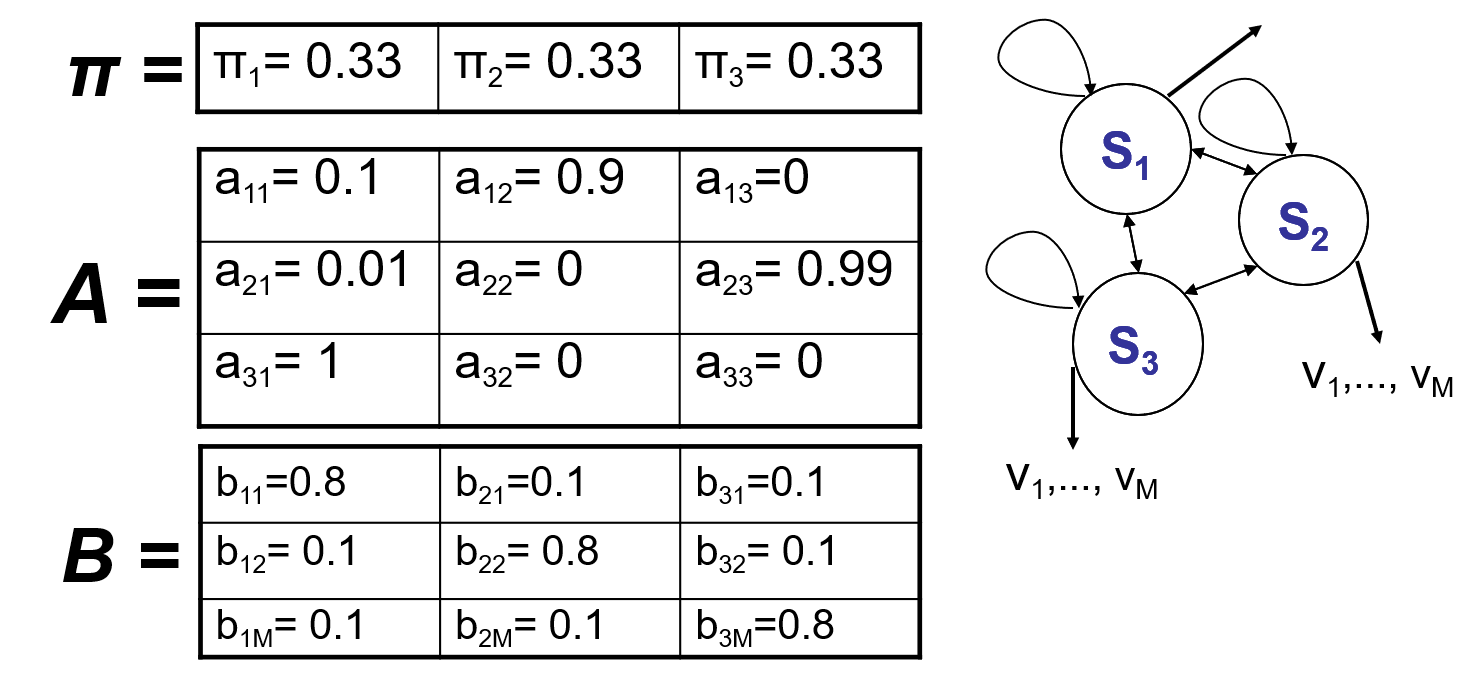
\includegraphics[width=\textwidth, height=\textheight, keepaspectratio]{hmm1.png}
\end{figure}

\subsection{Problemi chiave degli HMM}
I problemi chiave degli HMM sono:
\begin{enumerate}
    \item \textit{Evaluation}, per cui data una stringa di osservazioni $O=(O_1...O_t...O_T)$ si vuole calcolare $P(O|\lambda)$; questo problema si risolve con la \textit{procedura di forward}.
    \item \textit{Decoding}, per cui data una stringa di osservazioni $O$ e un modello HMM $\lambda$ si vuole calcolare la più probabile sequenza di stati $s_1...s_t$ che ha generato $O$; questo problema si risolve con l'\textit{algoritmo di Viterbi}.
    \item \textit{Training}, per cui dato un insieme di osservazioni $\{O\}$ si vuole determinare il miglior modello HMM $\lambda$, ovvero quello per cui $P(O|\lambda)$ è massimizzata; questo problema si risolve con l'\textit{algoritmo di Baum-Welch}.
\end{enumerate}
Alla base di tutti questi problemi sta il fatto che gli stati non sono direttamente osservabili.

\subsection{Procedura di forward}
\label{forward}
Data una serie di osservazioni, si potrebbe procedere per \textit{forza bruta}:
\[ P(O) = \sum_Q P(O,Q) = \sum_Q P(O|Q) \cdot P(Q) \]
dove $Q$ indica i cammini di lunghezza pari al numero di osservazioni. La probabilità a priori $P(Q)$ della sequenza di stati $Q$ sapremmo calcolarla: è la probabilità condizionata tra coppie di stati, ovvero $P(q_1) P(q_2|q_1) ... P(q_t|q_{t-1})$. La probabilità condizionata $P(O,Q)$ dell'osservazione dati gli stati, invece, si dovrebbe calcolare facendo la moltiplicazione delle probabilità di aver osservato un simbolo dato uno specifico stato, ovvero $P(O_1|q_1) P(O_2|q_2) ... P(O_t|q_t)$. Questo metodo, tuttavia, non è efficiente in quanto la sua complessità è pari a $O(tN^t)$.

Tramite la \textit{procedura di forward} è possibile ridurre la complessità computazionale delle operazioni appena presentate. Se si considerano le prime $t$ osservazioni $O_1, O_2, ..., O_t$ si ha che la probabilità
\[ \alpha_t(i) = P(O_1,O_2,...,O_t,q_t=s_i|\lambda) \]
è definibile ricorsivamente come:
\[ \alpha_1(i) = P(O_1,q_1=s_i) = P(q_1=s_i) \cdot P(O_1|q_1=s_i) = \pi_i \cdot b_i(O_1) \]
\begin{align*}
    \alpha_{t+1}(j) &= P(O_1,O_2,...,O_t,O_{t+1},q_{t+1}=s_j|\lambda) = \\
    &= \sum_{i=1}^N P(q_{t+1}=s_j|q_t=s_i) \cdot P(O_{t+1}|q_{t+1}=s_j) \cdot \alpha_t(i) = \\
    &= \sum_{i=1}^N [a_{ij} \cdot \alpha_t(i)] \cdot b_j(O_{t+1})
\end{align*}
Ne deriva che data la sequenza di osservazioni $O_1, O_2, ..., O_t, ..., O_T$ e conoscendo $\alpha_t(i)$ (variabile di forward) possiamo calcolare
\[ P(O_1,O_2,...,O_T) = \sum_{i=1}^N \alpha_T(i) \]
con una complessità computazionale pari a $O(TN^2)$. Oppure, in alternativa, si può calcolare ricorsivamente introducendo la variabile di backward
\[ \beta_t(j) = P(O_{t+1},...,O_T|q_t=s_j,\lambda) = \sum_{i=1}^N \beta_{t+1}(i) \cdot a_{ij} \cdot b_j(O_{t+1}) \]
da cui si ottiene:
\[ P(O|\lambda) = \sum_{j=1}^N \beta_0(j) \]
\begin{figure}[htp]
	\begin{subfigure}{0.49\textwidth}
	    \centering
		\includegraphics[width=\textwidth, height=\textheight, keepaspectratio]{hmm2.jpg}
		\caption{Algoritmo con variabile di forward}
	\end{subfigure}
	\hfill
	\begin{subfigure}{0.49\textwidth}
	    \centering
		\includegraphics[width=\textwidth, height=\textheight, keepaspectratio]{hmm3.jpg}
		\caption{Algoritmo con variabile di backward}
	\end{subfigure}
\end{figure}

\subsection{Algoritmo di Viterbi}
\label{Viterbi}
Il secondo problema è quello del decoding, ovvero quello di stabilire il cammino di stati più probabile che ha generato $O_1,O_2,...,O_T$.

Questo può essere espresso come $\argmax_Q P(Q|O_1,O_2,...,O_T)$. Quindi, una strategia di \textit{forza bruta} si potrebbe calcolare come:
\[ \argmax_Q \frac{P(O_1,O_2,...,O_T|Q) \cdot P(Q)}{P(O_1,O_2,...,O_T)} \]
In alternativa, un calcolo efficiente può essere fatto tramite l'\textit{algoritmo di Viterbi}. Tale algoritmo sfrutta infatti un approccio di programmazione dinamica che cerca il più probabile stato singolo alla posizione $i$-esima date le osservazioni e gli stati precedenti. Si vuole infatti trovare la singola migliore sequenza di stati singoli (path)
massimizzando la probabilità $P(Q|O,\lambda)$. L'algoritmo si articola in quattro fasi:
\begin{enumerate}
    \item \textit{Inizializzazione}, in cui si definiscono il caso base e il passo induttivo
    \[ \begin{cases}
    	\delta_1(i) = \pi_i \cdot b_i(O_1) & \text{con } 1 \leq i \leq N \\
    	\psi_1(i) = 0 &
    	\end{cases} \]
    \[ \delta_{t+1}(j) = [\max_i \delta_t(i) a_{ij}] \cdot b_j(O_{t+1}) \]
    
    \item \textit{Ricorsione}, in cui per ogni $1 \leq j \leq N$ abbiamo che
    \[ \delta_t(j) = \max_{1 \leq i \leq N} [\delta_{t-1}(i) a_{ij}] \cdot b_j(O_t) \]
    \[ \psi_t(j) = \argmax_{1 \leq i \leq N} [\delta_{t-1}(i) a_{ij}] \]
    
    \item \textit{Terminazione}, in cui arriviamo a
    \[ P^* = \max_{1 \leq i \leq N} [\delta_T(i)] \]
    \[ q_t^* = \argmax_{1 \leq i \leq N} [\delta_T(i)] \]
    
    \item \textit{Path backtracking}, in cui otteniamo per $t= T-1, T-2, ..., 1$
    \[ q_t^* = \psi_{t+1}(q_{t+1}^*) \]
\end{enumerate}
\begin{figure}[htp]
	\centering
	\includegraphics[width=0.4\textwidth]{hmm4.png}
\end{figure}

\subsection{Stima dei parametri di un HMM}
L'ultimo problema relativo agli HMM è il training. Tale problema è risolvibile tramite l'algoritmo di Baum-Welch oppure, in alternativa, si può usare anche l'approccio Maximum Likelihood. Nella \textit{procedura di ri-stima} di Baum-Welch si definiscono inizialmente due misure:
\[ \gamma_t(i) = P(q_t=s_i|O_1,O_2,...,O_T,\lambda) \]
\[ \xi_t(i,j) = P(q_t=s_i,q_{t+1}=s_j|O_1,O_2,...,O_T,\lambda) \]
Tali quantità possono essere calcolate in modo efficiente come
\[ \sum_{j=1}^N \xi_t(i,j) = \gamma_t(i) \]
dove:
\begin{itemize}
    \item $\sum_{t=1}^{T-1} \xi_t(i,j)$ è il numero atteso di transizioni dallo stato $i$ allo stato $j$ durante il cammino.
    \item $\sum_{t=1}^{T-1} \gamma_t(i)$ è il numero atteso di transizioni passanti dallo stato $i$ durante il cammino.
\end{itemize}
Queste quantità permettono di calcolare, per esempio, la stima di $P(s_j|s_i)$ come il loro rapporto $a_{ij}$.

Come per l'approccio Expectation-Maximization, utilizzando le variabili di forward e backward possiamo calcolare $\xi$ e $\gamma$ in due step:
\begin{itemize}
    \item \textit{Expectation}
    \[ \xi_t(i,j) = \frac{\alpha_t(i) a_{ij} b_j(O_{t+1}) \beta_{t+1}(j)}{P(O|\lambda)} = \frac{\alpha_t(i) a_{ij} b_j(O_{t+1}) \beta_{t+1}(j)}{\sum\limits_{i=1}^N \sum\limits_{j=1}^N \alpha_t(i) a_{ij} b_j(O_{t+1}) \beta_{t+1}(j)} \]

    \item \textit{Maximization}
    \[ \pi_i = \gamma_1(i) \]
    \[ a_{ij} = \frac{\sum\limits_{t=1}^{T-1} \xi_t(i,j)}{\sum\limits_{t=1}^{T-1} \gamma_t(i)} \]
    \[ b_j(k) = \frac{\sum\limits_{\substack{t=1 \\ t.c. \, O_t = v_k}}^{T} \gamma_t(j)}{\sum\limits_{t=1}^{T} \gamma_t(j)} \]
\end{itemize}
Le quantità appena descritte vengono utilizzate nel processo di stima dei parametri di un HMM in modo iterativo. Si utilizza quindi una variante dell'algoritmo EM che esegue un'ottimizzazione locale per \textit{massimizzare la log-likelihood} del modello rispetto ai dati.

\subsection{Algoritmo di Baum-Welch}
\label{BW}
Conoscendo le quantità che descrivono le frequenze attese degli stati e le transizioni da essi, si può costruire l'\textit{algoritmo di Baum-Welch} il quale si articola in cinque fasi:
\begin{enumerate}
    \item Inizializzo il modello $\bar{\lambda}=(A_0,B_0,\pi_0)$.
    \item Il modello corrente è $\lambda=\bar{\lambda}$.
    \item Uso il modello $\lambda$ per calcolare la parte destra delle formule di ri-stima (Expectation).
    \item Uso la statistica per la ri-stima dei parametri ottenendo il nuovo modello $\bar{\lambda}=(\bar{A},\bar{B},\bar{\pi})$ (Maximization).
    \item Vai al passo 2 finché non si verifica la terminazione (dopo un numero fissato di cicli oppure alla convergenza del valore di likelihood).
\end{enumerate}
\`{E} dimostrato che ad ogni passo $P(O_1,O_2,...,O_T|\bar{\lambda}) > P(O_1,O_2,...,O_T|\lambda)$. Si può quindi descrivere l'algoritmo di Baum-Welch come una tecnica di ottimizzazione a discesa del gradiente (ottimizzatore locale) in cui la log-likelihood è fortemente multimodale. Queste caratteristiche fanno capire quanto la scelta dei parametri per il training sia cruciale per la convergenza.
\begin{figure}[htp]
	\centering
	\includegraphics[width=0.4\textwidth]{hmm5.png}
\end{figure}

\section{Questioni aperte}
Nel campo del training degli HMM ci sono tre filoni di ricerca:
\begin{itemize}
    \item \textit{Selezione del modello}, quale topologia e quale numero di stati.
    \item \textit{Estensione dei modelli standard}, tramite modifica delle componenti e delle dipendenze.
    \item \textit{Inserimento di comportamenti discriminativi}.
\end{itemize}

\subsection{Selezione dell'ordine del modello}
Nella selezione dell'ordine del modello, da adottare quando si usano gli HMM, bisogna definire il numero di stati (tipicamente non è un grosso problema) e la topologia, ovvero il set di collegamenti tra gli stati.

Il problema della definizione del \textit{numero di stati} (tramite selezione di modelli standard) permette di evitare l'overfitting. La scelta del modello ottimale può avvenire per strategia forza bruta (si provano vari modelli e si sceglie quello che massimizza un certo criterio) o per maximum likelihood. Poiché il criterio della massimizzazione della log-likelihood può non funzionare (non decresce con l'aumentare dell'ordine del sistema), si inserisce un fattore penalizzante che cresce con l'aumentare dell'ordine del sistema, così da scoraggiare la scelta di un modello complesso. Sono esempi di \textit{penalized likelihood} i criteri BIC e AIC. Un approccio alternativo è basato sul modello split and merge, in cui a partire da modelli grossolani si prosegue con la loro divisione o unione ad altri fino ad ottenerne uno ottimale.
\begin{figure}[htp]
	\begin{subfigure}{0.49\textwidth}
	    \centering
		\includegraphics[width=\textwidth, height=\textheight, keepaspectratio]{hmm6.png}
		\caption{Definizione del numero di stati}
	\end{subfigure}
	\hfill
	\begin{subfigure}{0.49\textwidth}
	    \centering
		\includegraphics[width=\textwidth, height=\textheight, keepaspectratio]{hmm7.png}
		\caption{Penalized likelihood}
	\end{subfigure}
\end{figure}

\noindent
La definizione della \textit{topologia} si basa invece sul tipo di problema da affrontare. Soluzioni ad-hoc per questo problema sono per esempio: topologie a grafo completo (ergodic), collegamenti left to right e HMM circolari. Un'altra possibile soluzione è rappresentata dagli \textit{HMM sparsi}, ovvero grafi sparsi in cui componenti irrilevanti o ridondanti vengono pesate a zero.
\begin{figure}[htp]
	\begin{subfigure}{0.49\textwidth}
	    \centering
		\includegraphics[width=\textwidth, height=\textheight, keepaspectratio]{hmm8.png}
		\caption{Soluzioni per definire la topologia}
	\end{subfigure}
	\hfill
	\begin{subfigure}{0.49\textwidth}
	    \centering
		\includegraphics[width=\textwidth, height=\textheight, keepaspectratio]{hmm9.png}
		\caption{HMM sparsi}
	\end{subfigure}
\end{figure}

\subsection{Estensione dei modelli standard}
Una prima \textit{estensione dei modelli standard} può avvenire tramite aggiunta di dipendenze tra le componenti, così da modellare differenti comportamenti. Questa estensione si basa sul formalismo delle reti Bayesiane, in cui ogni nodo rappresenta una variabile e i link rappresentano le relazioni di causalità. Tre possibili estensioni sono:
\begin{enumerate}[label=(\alph*)]
    \item \textit{Input-output HMM}, in cui la sequenza di osservazioni dipende dallo stato nascosto e dall'input (che determina a sua volta lo stato).
    \item \textit{Factorial HMM}, in cui la sequenza di osservazioni dipende da più di una sequenza di stati nascosti.
    \item \textit{Coupled HMM}, costituite da una coppia di HMM che interagiscono fra loro.
\end{enumerate}
\begin{figure}[htp]
	\begin{subfigure}{0.3\textwidth}
        \centering
        \includegraphics[width=\textwidth, height=\textheight, keepaspectratio]{io-hmm.png}
        \caption{}
    \end{subfigure}
    \hfill
    \begin{subfigure}{0.3\textwidth}
        \centering
        \includegraphics[width=\textwidth, height=\textheight, keepaspectratio]{fact-hmm.png}
        \caption{}
    \end{subfigure}
    \hfill
    \begin{subfigure}{0.3\textwidth}
        \centering
        \includegraphics[width=\textwidth, height=\textheight, keepaspectratio]{coupled-hmm.png}
        \caption{}
    \end{subfigure}
\end{figure}

\noindent
In alternativa, si possono costruire delle funzioni per modellare i simboli in output sulla base di un \textit{sistema di emissione di probabilità}. Esempi di questa seconda possibile estensione sono: reti neurali, HMM gerarchici, kernel machines (SVM), factor analysis, distribuzioni Gaussiane generalizzate. Il problema di questa modalità di estensione è rappresentato dal fatto di dover fare il training per ogni tecnica adottata all'interno del framework. L'ottimalità si avrebbe con un training simultaneo dei parametri. Inoltre, se si utilizzano modelli a kernel (SVM) o reti neurali è necessario convertire il risultato del classificatore in un opportuno valore di probabilità.

\subsection{Inserimento di comportamenti discriminativi}
Il tipico problema nella modellazione dei classificatori è dato dalla divisione tra approccio generativo e discriminativo. L'approccio \textit{generativo} (HMM) costruisce un modello per ogni classe/gruppo fornendo soluzioni migliori nella descrizione delle classi. L'approccio \textit{discriminativo} (SVM), invece, costruisce un unico modello per separare tutte le classi/gruppi fornendo soluzioni migliori al problema in esame.
\begin{figure}[htp]
	\begin{subfigure}{0.49\textwidth}
	    \centering
		\includegraphics[width=0.5\textwidth]{gen.png}
		\caption{Approccio generativo}
	\end{subfigure}
	\hfill
	\begin{subfigure}{0.49\textwidth}
	    \centering
		\includegraphics[width=0.5\textwidth]{discr.png}
		\caption{Approccio discriminativo}
	\end{subfigure}
\end{figure}

\noindent
Dato che gli HMM sono un modello generativo, l'inserimento di informazioni discriminative (provenienti direttamente dalle classi) può essere fatto in fase di training o in fase di classificazione. Il \textit{training discriminativo} degli HMM si basa sull'idea di addestrare il modello tramite un criterio discriminativo, considerando ad esempio le informazioni provenienti da altre classi. Infine, mentre nella classificazione standard prima si addestra un HMM per ogni classe e poi si applica la regola di Bayes, nella \textit{classificazione discriminativa} si usa un HMM addestrato per definire uno spazio delle features dove addestrare poi un classificatore discriminativo. I tipi di features da trattare in questo caso possono essere la log-likelihood o il suo gradiente.
\begin{figure}[htp]
	\begin{subfigure}{0.49\textwidth}
	    \centering
		\includegraphics[width=\textwidth, height=\textheight, keepaspectratio]{std-class.png}
		\caption{Classificazione standard}
	\end{subfigure}
	\hfill
	\begin{subfigure}{0.49\textwidth}
	    \centering
		\includegraphics[width=\textwidth, height=\textheight, keepaspectratio]{discr-class.png}
		\caption{Classificazione discriminativa}
	\end{subfigure}
\end{figure}

\section{Sommario}
Un \textit{processo di Markov} si può vedere come un automa a stati finiti in cui la transizione da uno stato all'altro avviene con una certa probabilità. Tale probabilità dipende solamente dallo stato immediatamente precedente e non dall'intera storia degli stati passati (Markovianità del primo ordine).

Un \textit{modello di Markov} a $N$ stati può essere rappresentato tramite una matrice $A = \{ a_{ij} \}$ di dimensione $N \times N$. Ogni elemento $a_{ij}$ della matrice corrisponde alla probabilità di transizione dallo stato $i$ allo stato $j$. Dato che questi valori rappresentano delle probabilità, la somma di ogni riga della matrice di transizione deve essere pari a 1. Per completare il modello, è necessario definire anche la distribuzione di probabilità $\pi$ degli stati iniziali, ovvero le probabilità di trovarsi in un determinato stato all'inizializzazione della macchina a stati. Anche la somma di queste probabilità deve essere pari a 1.

Un \textit{Hidden Markov Model} è un modello di Markov in cui non è possibile osservare direttamente lo stato corrente, per via del fatto che gli stati sono nascosti. Tuttavia, è possibile ottenere l'osservazione legata ad un certo stato. Infatti, ad ogni valutazione della macchina a stati, lo stato corrente $s_j$ produrrà un simbolo $v_k$ in uscita, il quale dipenderà da una distribuzione di probabilità $B = \{ b_j(v_k) \}$. Ovvero $P(v_k|s_j)$ è la probabilità di emissione del simbolo $v_k$ quando lo stato del sistema è $s_j$. In sostanza, un HMM (discreto e addestrato) è descritto dai seguenti parametri:
\begin{itemize}
    \item Una matrice di transizione $A = \{ a_{ij} \}$.
    \item Una distribuzione di probabilità sui simboli di osservazione $B = \{ b_j(v_k) \}$.
    \item Una distribuzione di probabilità degli stati iniziali $\pi = \{ \pi_i \}$.
\end{itemize}
\newpage
\noindent
Data una sequenza di osservazioni $O = (O_1, O_2, ..., O_t)$ ed un HMM $\lambda$ noto, è possibile ottenere, tramite la \hyperref[forward]{\textit{procedura di forward}}, un valore che descrive la probabilità che tale sequenza sia stata generata dal modello in questione. Questo valore, denominato \textit{likelihood} (verosimiglianza), è scritto come $P(O | \lambda)$. Invece, se si desidera conoscere la sequenza di stati più probabile, è possibile utilizzare l'\hyperref[Viterbi]{\textit{algoritmo di Viterbi}}, il quale restituisce la likelihood lungo la sequenza di stati più probabile. Infine, per determinare il miglior modello HMM (quello per cui $P(O|\lambda)$ è massimizzata), si deve utilizzare l'\hyperref[BW]{\textit{algoritmo di Baum-Welch}}. Questo algoritmo non ha bisogno di conoscere gli stati associati alle osservazioni. Infatti, partendo da un modello iniziale (una stima), l'algoritmo esegue iterativamente una procedura di Expectation-Maximization convergendo ad un massimo locale della likelihood. Dato che i parametri trovati corrispondono ad un massimo locale (e non globale) la stima iniziale dei parametri del modello può influenzare fortemente il risultato. Tuttavia, l'algoritmo trova una soluzione soddisfacente nella maggior parte dei casi.

La selezione del modello è una questione aperta nel campo del \textit{training} degli HMM. Infatti, per costruire un HMM è necessario definire il numero dei suoi stati e la sua topologia. Per la scelta del \textit{numero di stati} non esiste una regola precisa:
\begin{itemize}
    \item Si può scegliere un valore che si crede ragionevole per l'applicazione.
    \item Si possono fare più tentativi per trovare il numero di stati che massimizza un certo criterio (brute force).
    \item Si può scegliere il valore che massimizza la log-likelihood (anche utilizzando fattori penalizzanti per evitare la scelta di un modello troppo complesso).
    \item Si può partire da un modello grossolano e dividerlo/unirlo ad altri fino a che non se ne ottiene uno ottimale.
\end{itemize}
Per \textit{topologia}, invece, si intende l'insieme delle transizioni ammesse dal modello (collegamenti tra stati). Soluzioni ad-hoc per la scelta della topologia sono: topologie a grafo completo, collegamenti left to right, HMM circolari, HMM sparsi.


\chapter{Classificatori discriminativi}

\section{Introduzione}
I classificatori \textit{generativi}:
\begin{itemize}
    \item Modellano le probabilità condizionali (likelihood) e a priori delle classi per ogni classe (indipendentemente).
    \item Usano la regola di decisione di Bayes per classificare, prendendo la massima posterior.
\end{itemize}
I classificatori \textit{discriminativi}:
\begin{itemize}
    \item Stimano direttamente il confine di decisione, producendo una stima di classificazione.
    \item Sono approcci geometrici (anche se non è semplice trovare un parallelismo con la regola di Bayes).
\end{itemize}

\section{Funzioni discriminanti lineari}
In un problema binario, l’obiettivo è trovare la retta che separa le due classi. Un approccio di questo tipo è stato visto finora solo per le distribuzioni gaussiane; il compito è ora quello di generalizzare. Si parla di \textit{funzione discriminante lineare} quando la funzione discriminante è combinazione lineare delle varie features. Definiamo quindi la funzione discriminante lineare $g: \mathbb{R}^d \rightarrow \mathbb{R}$ come:
\[ g(x') = w^{'t} x' + w_0 \]
dove $x'=[x_1,...,x_d]$, $w'=[w_1,...,w_d]$ sono i pesi e $w_0$ è il termine noto (o bias). Un campione $x'$ è classificato come appartenente alla classe $\omega_1$ se $w^{'t} x' + w_0 > 0$, altrimenti se $w^{'t} x' + w_0 < 0$ verrà classificato come appartenente alla classe $\omega_2$. Geometricamente, settando $g(x')=0$ si ottiene un \textit{iperpiano} (o superficie di separazione). Infatti, $w'$ determina l'orientazione del piano e, assieme a $w_0$, la distanza del piano rispetto all'origine.
\begin{figure}[htp]
	\centering
	\includegraphics[width=0.9\textwidth]{svm1.png}
\end{figure}

\subsection{Training}
Più genericamente, considerando $w=[w_0,w_1,...,w_d]$ e $x=[1,x_1,...,x_d]$, la regola di decisione diventa: un campione $x$ è classificato come appartenente alla classe $\omega_1$ se $w^t x > 0$, altrimenti se $w^t x < 0$ verrà classificato come appartenente alla classe $\omega_2$. Dato quindi come \textit{training set} un insieme di $N$ campioni $x'_1,...,x'_N$ alcuni etichettati $\omega_1$ ed altri etichettati $\omega_2$, si vogliono determinare il vettore dei pesi $w'$ e il termine $w_0$ della funzione discriminante lineare. Un ragionevole approccio è la ricerca di un vettore di pesi tale che la probabilità di commettere errore sui campioni sia minima. Se esiste un vettore di pesi tale da rendere nulla la probabilità di errore, allora i campioni si dicono \textit{linearmente separabili}.
\begin{figure}[htp]
	\centering
	\includegraphics[width=0.9\textwidth]{svm2.png}
\end{figure}

\noindent
L'obiettivo è quindi quello di calcolare pesi che soddisfino le seguenti condizioni:
\[ \forall x \in \omega_1. \, w^t x > 0 \]
\[ \forall x \in \omega_2. \, w^t x < 0 \]
Nella seconda condizione si può anche dire che $x$ è classificato correttamente se $w^t (-x) > 0$. Ciò suggerisce una \textit{normalizzazione} (cambiare il segno a tutti gli oggetti della classe $\omega_2$) che semplifica il trattamento nel caso di due diverse classi, ossia il fatto che si possa solo trovare il vettore dei pesi tale per cui si abbia $w^t x > 0$ per tutti i campioni a prescindere dalle classi. Questo vettore $w$ è chiamato \textit{vettore soluzione} (o separatore).

Risulta chiaro che se il vettore soluzione esiste, esso non è unico. Ci saranno quindi diversi modi per imporre requisiti addizionali per vincolare il vettore soluzione. Uno potrebbe essere quello di cercare il vettore dei pesi che massimizzi la minima distanza dei campioni dal piano separatore. Un altro potrebbe essere quello di cercare il vettore dei pesi che soddisfi $w^t x \geq b$, dove $b$ è una costante positiva chiamata \textit{margine}. 

\subsection{Tecnica del gradiente discendente}
Per determinare il vettore dei pesi $w$ si ricorre a tecniche di minimizzazione, le quali minimizzano un funzionale in funzione di certe quantità. Una delle tecniche di base è quella del \textit{gradiente discendente}, ossia uno degli approcci più semplici per il calcolo di una funzione discriminante. La tecnica del gradiente discendente è un metodo iterativo di assestamento progressivo dei pesi che si basa sulla seguente proprietà: il vettore gradiente nello spazio $W$ (ossia i coefficienti di $w$) punta nella direzione di massimo scarto di una funzione da minimizzare.

La \textit{procedura} consiste nell'aggiornare il valore del vettore dei pesi al passo $k+1$ con un contributo proporzionale al modulo del gradiente di un particolare funzionale al passo precedente. Tale procedura può essere formulata come:
\[ w(k+1) = w(k) - \rho_k \nabla J(w) |_{w=w(k)} \]
dove $J(w)$ è la funzione di valutazione che deve essere minimizzata. Questa funzione deve essere scelta in modo tale che raggiunga il suo minimo quanto più $w$ si avvicina alla soluzione ottima (nel caso in cui essa sia convessa). Quindi, il minimo di $J(w)$ si ottiene spostando $w$ in direzione opposta al gradiente.

Chiaramente occorre scegliere un \textit{criterio di ottimalità}. La scelta più ovvia è quella di definire un funzionale $J(w;x_1,...,x_N)$ rappresentato dal numero di campioni mal classificati da $w$ su un totale di $N$ campioni (error rate). Siccome tale funzionale è costante a tratti, il metodo della discesa del gradiente non è molto adatto a tale problema. Una scelta migliore per $J$ può essere perciò:
\[ J(w) = - \sum_{i \in X} w^t x_i \]
dove $X$ è l'insieme di punti classificati non correttamente da $w$. Geometricamente, $J(w)$ è proporzionale alla somma delle distanze dei campioni mal classificati dal confine di decisione. Siccome $\nabla J = - \sum_{i \in X} x_i$, l'algoritmo di discesa del gradiente diventa:
\[ w(k+1) = w(k) + \rho_k \cdot \sum_{i \in X} x_i \]
con $\rho_k = \frac{1}{k}$.

Si citano infine altri metodi per scegliere $J(w)$ e ottimizzarla: metodo del rilassamento, metodo del MSE (Minimum Square Error), metodo del Least-MSE (o Widrow-Hoff), metodo di Ho-Kashyap, stochastic gradient.

\subsection{Funzioni discriminanti lineari generalizzate}
Nel caso di problemi a $C$ classi, possono essere costruiti $C-1$ classificatori $g_j(x)$, uno per ogni problema $C_j$ vs \textit{non-}$C_j$ (one-vs-rest). Oppure si possono costruire $C(C-1)/2$ classificatori binari che classificano un punto a maggioranza (one-vs-one). La funzione discriminante lineare può anche essere scritta come:
\[ g(x) = w_0 + \sum_{i=1}^d w_i x_i \]
dove $w_i$ è la componente $i$-esima del vettore dei pesi e $w_0$ è il solito termine noto. Possiamo quindi aggiungere altri termini in cui mettiamo i prodotti delle varie componenti di $x$, ad esempio un classificatore discriminante quadratico sarà nella forma:
\[ g(x) = w_0 + \sum_{i=1}^d w_i x_i + \sum_{i=1}^d \sum_{j=1}^d v_{ij} x_i x_j \]
Possiamo infine \textit{generalizzare} il concetto scrivendo:
\[ g(x) = \sum_{k=1}^K a_k \cdot y_k(x) \]
dove $y_k$ sono funzioni arbitrarie su $x$ che possono essere viste direttamente come nuove features. In altre parole, le funzioni $y_k$ possono essere viste come \textit{estrattori di features}. Di solito, la fase di estrazione delle features viene usata per diminuire la dimensionalità (PCA), mentre qui viene usata per aumentarla.

La funzione discriminante lineare generalizzata $g(x)$ è lineare nello spazio di $y$ (è una funzione semplice) e non lineare nello spazio originale di $x$ (è una funzione complessa). Per esempio, con la funzione $g(x) = a_1 + a_2 x + a_3 x^2$ si passa da uno spazio delle features monodimensionale ad uno spazio tridimensionale.
\begin{figure}[htp]
	\centering
	\includegraphics[width=0.85\textwidth]{svm3.png}
\end{figure}

\section{Support Vector Machines}
Le \textit{Support Vector Machines} (SVM) possono essere viste come separatori lineari (ipotizzando un problema linearmente separabile), ereditando la notazione vista finora, dove $b=w_0$ indica il margine. Per la classificazione basta applicare il segno alla funzione discriminante:
\[ f(x) = sign(w^T x + b) =
    \begin{cases}
        +1 \\
        -1
    \end{cases} \]
Per trovare il separatore ottimo, chiamo $r$ la distanza di un campione dall'iperpiano e chiamo \textit{support vectors} i campioni più vicini all'iperpiano (tale definizione verrà poi generalizzata). Il margine dell'iperpiano $h$ di separazione è la somma delle distanze minime dei campioni su di esso. Individuare l’iperpiano $h$ ottimo corrisponde a massimizzare il margine. Questo implica che solo alcuni esempi sono importanti per l'apprendimento (i vettori di supporto SV), gli altri invece possono essere ignorati.
\begin{figure}[htp]
	\centering
	\includegraphics[width=0.55\textwidth]{svm4.png}
\end{figure}

\subsection{Addestramento di una SVM}
L'addestramento della SVM consiste nel trovare il vettore $w$ e il parametro $b$ ottimali (che massimizzino il margine), a partire dal training set. Si hanno quindi i dati di addestramento $D \{(x_i, y_i) \}$ (dove $\{y\}$ indica label binarie di valore 1 o -1), a distanza almeno 1 dall'iperpiano, su cui valgono le seguenti condizioni:
\begin{align*}
    w^T x_i + b \geq 1 \, &se \, f(x_i)=+1 \\
    w^T x_i + b \leq -1 \, &se \, f(x_i)=-1
\end{align*}
Per i vettori di supporto la disuguaglianza diventa una uguaglianza, perché essi stanno esattamente a distanza 1 dall'iperpiano separatore.

Le variabili incognite del problema sono il vettore $w$ perpendicolare al piano di separazione (si suppone $w$ versore per comodità) e la distanza $b=b/||w||$ del piano dall'origine. Indichiamo quindi con $\rho$ la distanza fra i piani $P^+: w^T x_i + b = 1$ e $P^-: w^T x_i + b = -1$. Se $x^+$ è un punto di $P^+$ e $x^-$ è un punto di $P^-$ a distanza minima da $x^+$, allora posso scrivere $\rho = |x^+ - x^-|$, e posso anche scrivere $(x^+ - x^-) = \lambda w$. Essendo $x^+$ e $x^-$ a distanza minima, muoversi da $x^+$ a $x^-$ corrisponde a muoversi lungo un percorso $x^+ = x^- + \lambda w$ nella direzione di $w$ e di lunghezza $||\lambda w||$.
\begin{figure}[htp]
	\centering
	\includegraphics[width=0.55\textwidth]{svm5.png}
\end{figure}

\subsection{SVM lineari}
Mettendo assieme quanto visto nella sezione precedente, vogliamo capire chi sia $\rho$. Isolando $\lambda$ e $w$ da $x^+ = x^- + \lambda w$ e sfruttando le uguaglianze $w^T x_i + b = 1$ e $w^T x_i + b = -1$ otteniamo:
\[ \rho = \left| \left| \frac{2}{w^T w} \cdot w \right| \right| = \left| \left| \frac{2}{w^T} \right| \right| = \frac{2}{||w||} \]
Per massimizzare il margine dovremo quindi minimizzare $||w||$. Il \textit{problema di ottimizzazione} quadratica che ne risulta è illustrato (in due diverse formulazioni) nelle figure sottostanti.
\begin{figure}[htp]
	\begin{subfigure}{0.49\textwidth}
	    \centering
		\includegraphics[width=\textwidth, height=\textheight, keepaspectratio]{svm-lin1.png}
		\caption{Problema di ottimizzazione}
	\end{subfigure}
	\hfill
	\begin{subfigure}{0.49\textwidth}
	    \centering
		\includegraphics[width=\textwidth, height=\textheight, keepaspectratio]{svm-lin2.png}
		\caption{Formulazione duale}
	\end{subfigure}
\end{figure}

\noindent
Quindi, per risolvere questo problema di ottimizzazione, si deve ottimizzare una funzione quadratica soggetta a vincoli lineari (uno per ogni $x_i$): $y_i (w^T x_i + b) \geq 1$. Siccome i problemi di ottimizzazione quadratica sono problemi di programmazione matematica ben noti, esistono diversi algoritmi; uno di questi comporta l'utilizzo dei moltiplicatori di Lagrange ed è illustrato nella prossima figura.
\begin{figure}[htp]
	\centering
	\includegraphics[width=0.9\textwidth]{svm-lin3.png}
\end{figure}
\newpage
\noindent
Usando le equazioni trovate al punto 3 nel punto 2, attraverso alcuni passaggi (\textit{figura (a)}), otteniamo la formulazione finale (\textit{figura (b)}).
\begin{figure}[htp]
	\begin{subfigure}{0.49\textwidth}
	    \centering
		\includegraphics[width=\textwidth, height=\textheight, keepaspectratio]{svm-lin4.png}
		\caption{}
	\end{subfigure}
	\hfill
	\begin{subfigure}{0.49\textwidth}
	    \centering
		\includegraphics[width=\textwidth, height=\textheight, keepaspectratio]{svm-lin5.png}
		\caption{}
	\end{subfigure}
\end{figure}

\subsection{Margini soft}
Se il set di addestramento non è linearmente separabile, si introducono le cosiddette \textit{slack variables} $\xi_i$ per consentire la classificazione errata di qualche punto. Nel problema di ottimizzazione con le slack variables viene introdotto il parametro $C$ che pesa gli errori e controlla l'overfitting (più $C$ è piccolo più ammetto errori). I valori di $\xi_i$ si interpretano come:
\begin{itemize}
    \item $\xi_i = 0$, classificazione corretta.
    \item $0 < \xi_i < 1$, classificazione corretta ma oltre il margine.
    \item $\xi_i \geq 1$, errore di classificazione.
\end{itemize}
Il sistema vincolato viene ancora risolto nella sua forma duale ed il risultato è ancora $w = \sum_{i=1}^N \alpha_i y_i x_i$, ma ora i support vectors saranno:
\begin{itemize}
    \item I punti per cui $\alpha_i$ è diverso da zero.
    \item I punti sul margine.
    \item I punti classificati correttamente ma oltre il margine.
    \item I punti classificati non correttamente.
\end{itemize}
\begin{figure}[htp]
	\begin{subfigure}{0.49\textwidth}
	    \centering
		\includegraphics[width=\textwidth, height=\textheight, keepaspectratio]{svm-lin6.png}
		\caption{Slack variables}
	\end{subfigure}
	\hfill
	\begin{subfigure}{0.49\textwidth}
	    \centering
		\includegraphics[width=\textwidth, height=\textheight, keepaspectratio]{svm-lin7.png}
		\caption{Classificazione soft margin}
	\end{subfigure}
\end{figure}

\subsection{SVM non lineari}
Se il problema non è linearmente separabile, l'idea è quella di proiettare le features in uno spazio nel quale i dati risultino separabili. I problemi di questa \textit{proiezione ad alta dimensionalità} sono:
\begin{itemize}
    \item Proiettare i punti in uno spazio a dimensionalità troppo elevata può portare alla curse of dimensionality.
    \item La complessità computazionale aumenta.
    \item Lo spazio risultante è quasi vuoto.
    \item Potrebbero in teoria esserci anche mapping in grado di proiettare i punti in uno spazio a dimensionalità infinita.
    \item Scegliere il mapping corretto potrebbe non essere facile.
\end{itemize}
\begin{figure}[htp]
	\centering
	\includegraphics[width=\textwidth, height=\textheight, keepaspectratio]{svm6.png}
\end{figure}

\subsection{Kernel trick}
Il problema di ottimizzazione visto per le SVM lineari produce come risultato:
\[ w = \sum_{i=1}^N \alpha_i y_i x_i \]
Siccome in fase di testing la \textit{classificazione} avviene con $f(x)=sign(w^Tx+b)$, possiamo scrivere:
\[ f(x) = sign \left( \left[ \sum_{i=1}^N \alpha_i y_i x_i \right]^T \cdot x + b \right) = sign \left( \sum_{i=1}^N \alpha_i y_i x_i^T x + b \right) \]
Quindi, i punti del training set (nel training e nel testing di una SVM) non appaiono mai da soli ma sempre in \textit{prodotto scalare} con altri punti. Applicando il mapping $\Phi(x)$ per proiettare i punti in uno spazio a dimensionalità maggiore si ottiene:
\[ w^Tx = \sum_{i=1}^N \alpha_i y_i \Phi(x_i^T) \Phi(x) \]
Le \textit{funzioni kernel} permettono di evitare di calcolare il prodotto in uno spazio ad elevata dimensionalità. Una funzione kernel corrisponde quindi ad un prodotto scalare in uno spazio esteso. Siccome il classificatore lineare si basa sul prodotto scalare fra vettori dello spazio delle istanze $X$ (non esteso) $K(x_i,x_j) = x_i^T x_j$, se ogni punto di $D$ è traslato in uno spazio di dimensioni maggiori attraverso una trasformazione $\Phi(x)$, il prodotto scalare diventa:
\[ K(x_i,x_j) = \Phi(x_i)^T \Phi(x_j) = x'^T_i x'_j \]
dove $x'$ indica una trasformazione non lineare. Si ottiene infine:
\[ w^Tx = \sum_{i=1}^N \alpha_i y_i K(x_i,x) \]
Per alcune funzioni, verificare che $K(x_i,x_j) = \Phi(x_i)^T \Phi(x_j)$ è complesso. Sono \textit{esempi} di funzioni kernel:
\begin{itemize}
    \item Funzione lineare, $K(x_i,x_j) = x_i^T x_j$.
    \item Funzione polinomiale di potenza $p$, $K(x_i,x_j) = (1 + x_i^T x_j)^p$.
    \item Funzione Gaussiana (Radial Basis Function), $K(x_i,x_j) = e^{- \frac{||x_i-x_j||^2}{2 \sigma^2}}$.
    \item Percettrone a due stadi (sigmoide), $K(x_i,x_j) = \tanh (\beta_0 x_i^T x_j + \beta_1)$.
\end{itemize}
In generale, ogni funzione semi-definita positiva è un kernel (teorema di Mercer).

\newpage
\subsection{Selezione del kernel}
Il kernel \textit{lineare}:
\begin{itemize}
    \item Viene utilizzato quando lo spazio delle features è già molto grande; ad esempio nella classificazione del testo, che utilizza i conteggi delle singole parole come features.
    \item \`{E} un caso speciale del kernel RBF.
    \item Non richiede parametri aggiuntivi. 
\end{itemize}
Il kernel \textit{polinomiale}:
\begin{itemize}
    \item Va in difficoltà in presenza di valori che si avvicinano allo zero o all'infinito.
    \item \`{E} una buona scelta in ambiti ben noti e ben condizionati.
    \item Ha un parametro aggiuntivo, ossia il grado $p$.
\end{itemize}
Il kernel \textit{RBF} (Radial Basis Function):
\begin{itemize}
    \item Viene indicato in generale come la scelta migliore.
    \item Ha bisogno del parametro aggiuntivo $\sigma$.
\end{itemize}
Il kernel \textit{sigmoide}:
\begin{itemize}
    \item Ha bisogno di due parametri aggiuntivi, ossia $\beta_0$ e $\beta_1$.
    \item Per alcuni valori di $\beta_0$ e $\beta_1$ non soddisfa il teorema di Mercer.
    \item Deriva dalle reti neurali.
    \item Non viene consigliato dalla letteratura.
\end{itemize}
\begin{figure}[htp]
	\begin{subfigure}{0.3\textwidth}
        \centering
        \includegraphics[width=\textwidth, height=\textheight, keepaspectratio]{kernel1.png}
        \caption{Lineare}
    \end{subfigure}
    \hfill
    \begin{subfigure}{0.3\textwidth}
        \centering
        \includegraphics[width=\textwidth, height=\textheight, keepaspectratio]{kernel2.png}
        \caption{Polinomiale grado 3}
    \end{subfigure}
    \hfill
    \begin{subfigure}{0.3\textwidth}
        \centering
        \includegraphics[width=\textwidth, height=\textheight, keepaspectratio]{kernel3.png}
        \caption{RBF con $\sigma=1$}
    \end{subfigure}
\end{figure}

\subsection{Sommario}
Nel caso di una SVM lineare, il classificatore (funzione obiettivo) è un iperpiano di separazione. I punti più importanti sono i \textit{vettori di supporto}, così chiamati per il fatto che sostengono l'iperpiano mantenendolo in equilibrio. Algoritmi di ottimizzazione quadratica identificano quali punti rappresentano il supporto. Nella formulazione di questo \textit{problema di ottimizzazione} appaiono i prodotti scalari. Se i dataset non sono separabili si può proiettare il problema in uno spazio di dimensioni maggiori (SVM non lineari).
\newpage
\noindent
Le SVM sono attualmente fra i migliori classificatori in una varietà di problemi. I \textit{vantaggi} delle SVM sono:
\begin{itemize}
    \item Hanno un'interpretazione geometrica semplice.
    \item Il kernel trick permette di ottenere in modo efficiente un classificatore non lineare senza incorrere nella curse of dimensionality.
    \item La soluzione del training è ottimale.
    \item I support vectors danno una rappresentazione compatta del training set; il loro numero fornisce infatti un'idea della capacità di generalizzazione (meno sono e meglio è).
    \item In moltissimi contesti applicativi funzionano decisamente bene; la teoria alla base delle SVM (statistical learning theory) è infatti elegante e solida.
\end{itemize}
Gli \textit{svantaggi}, invece, sono:
\begin{itemize}
    \item La scelta di kernel e parametri è cruciale.
    \item A volte il training può essere oneroso in termini di tempo.
    \item Il training non è incrementale, ovvero se arriva un nuovo oggetto occorre rifare da capo tutto l'addestramento.
    \item La gestione del caso multiclasse non è ottimale (sia in termini di efficienza che in termini di soluzione proposta).
\end{itemize}
Il \textit{tuning} dei parametri di una SVM è un'arte. Infatti, la selezione di uno specifico kernel e dei parametri viene spesso eseguita in modo empirico (tenta e verifica). Una possibile ricetta è:
\begin{enumerate}
    \item Esegui un semplice ridimensionamento dei dati (ad es. z-normalizzazione).
    \item Considera il kernel RBF.
    \item Usa la cross-validazione per trovare i migliori $C$ e $\sigma$.
    \item Usa i migliori $C$ e $\sigma$ per allenare l'intero training set.
    \item Verifica. 
\end{enumerate}
Vediamo infine alcuni problemi di questa ricetta e le relative soluzioni.
\begin{itemize}
    \item La ricerca dei parametri può richiedere molto tempo; soluzione: condurre la ricerca dei parametri in modo gerarchico.
    \item A volte i kernel RBF sono soggetti a overfitting; soluzione: usare kernel polinomiali di alto grado.
    \item La ricerca dei parametri deve essere ripetuta per ogni feature scelta (non c'è riuso dei calcoli); soluzione: confrontare le features su sottoinsiemi casuali dell'intero dataset per contenere i costi di computazione.
    \item Gli intervalli di ricerca per $C$ e $\sigma$ sono difficili da scegliere; soluzione: provare valori crescendo esponenzialmente, ad esempio $C=2^{[-5...15]}$ e $\sigma=2^{[-15...5]}$.
\end{itemize}


\chapter{Clustering}

\section{Introduzione}
Il \textit{clustering} è un metodo di classificazione che prevede il raggruppamento degli oggetti studiati secondo gruppi naturali, ovvero caratterizzati da features con valori simili. Ciò comporta che gli oggetti possono essere di classi diverse ma vicini nello spazio delle features. La differenza principale con i metodi di classificazione visti finora sta nel fatto che il fattore discriminante è la similarità tra gli oggetti.

\section{Classi di approcci}
A seconda del \textit{punto di vista} adottato possiamo avere differenti tipologie (classi) di clustering.
\begin{itemize}
    \item Tipo di risultato dell'operazione di clustering:
    \begin{itemize}
        \item Clustering \textit{gerarchico}, ritorna una serie di partizioni innestate (dendrogramma) e, tramite l'uso di matrici di prossimità, mira ad evidenziare le relazioni tra i vari pattern del dataset; non dovendo impostare il numero di clusters a priori permette un partizionamento più informativo, ma non è trattabile per dataset grandi; alcuni esempi sono complete link, single link e ward link.
        \item Clustering \textit{partizionale}, ritorna una singola partizione dei dati (il numero di clusters è dato a priori) mirando a identificare i gruppi naturali presenti nel dataset a partire da dati in forma vettoriale; nonostante sia ottimo per dataset grandi, il problema è scegliere il numero di clusters; alcuni esempi sono K-means e le sue varianti PAM e ISODATA.
    \end{itemize}
    \item Natura dei clusters risultanti:
    \begin{itemize}
        \item \textit{Hard clustering}, associa ad ogni pattern un unico cluster (per questo è detto anche clustering esclusivo); un esempio di problema è il raggruppamento delle persone per età.
        \item \textit{Soft clustering}, permette di associare un pattern a più clusters (clustering non esclusivo); un esempio è il raggruppamento delle persone per malattia.
    \end{itemize}
    \item Come vengono formati i clusters:
    \begin{itemize}
        \item Clustering \textit{agglomerativo}, si costruiscono i clusters tramite operazioni di merge, inizializzando ogni pattern con un cluster, fino al raggiungimento di una determinata condizione.
        \item Clustering \textit{divisivo}, opera invece con operazioni di split, partendo da un unico cluster.
    \end{itemize}
    \item Come vengono processati i pattern:
    \begin{itemize}
        \item Clustering \textit{sequenziale}, i pattern vengono processati uno alla volta.
        \item Clustering \textit{simultaneo}, i pattern vengono processati tutti assieme.
    \end{itemize}
    \item Come vengono utilizzate le features:
    \begin{itemize}
        \item Clustering \textit{monothetic}, viene utilizzata una feature alla volta per fare clustering.
        \item Clustering \textit{polythetic}, vengono utilizzate tutte le features simultaneamente per fare clustering (la maggior parte delle tecniche di clustering sono polythetic).
    \end{itemize}
    \item Come viene formulato matematicamente l'algoritmo:
    \begin{itemize}
        \item \textit{Graph theory}, gli algoritmi sono formulati in termini di teoria dei grafi e ne utilizzano definizioni e proprietà (ad esempio la connettività).
        \item \textit{Matrix algebra}, gli algoritmi sono espressi in termini di formule algebriche (ad esempio l'errore quadratico medio).
    \end{itemize}
    \item Quando arrivano nuovi dati:
    \begin{itemize}
        \item Clustering \textit{incrementale}, è possibile aggiornare il clustering fino ad ora costruito (caratteristica cruciale in questi anni dove i dataset sono sempre più grandi e in espansione).
        \item Clustering \textit{non incrementale}, non permette l'aggiornamento e per questo necessita di riesaminare completamente l'intero dataset.
    \end{itemize}
    \item Come viene ottimizzata la funzione di errore:
    \begin{itemize}
        \item Clustering \textit{deterministico}, effettua un'ottimizzazione classica (discesa lungo il gradiente).
        \item Clustering \textit{stocastico}, fa una ricerca stocastica nello spazio degli stati della soluzione (Monte Carlo).
    \end{itemize}
\end{itemize}
\begin{figure}[htp]
	\begin{subfigure}{0.49\textwidth}
	    \centering
		\includegraphics[width=\textwidth, height=\textheight, keepaspectratio]{clustering3.png}
		\caption{Clustering gerarchico vs partizionale}
	\end{subfigure}
	\hfill
	\begin{subfigure}{0.49\textwidth}
	    \centering
		\includegraphics[width=\textwidth, height=\textheight, keepaspectratio]{clustering4.png}
		\caption{Clustering monothetic}
	\end{subfigure}
\end{figure}

\section{Clustering partizionale}
Per quanto riguarda il clustering partizionale, ci sono ulteriori classi di approcci:
\begin{itemize}
    \item Clustering \textit{sequenziale}, ossia un approccio semplice ed intuitivo ottimo per cluster convessi in cui (tipicamente) i pattern sono processati poche volte; il risultato finale in genere dipende dall'ordine con cui sono presentati i pattern.
    \item \textit{Center-based} clustering, in cui ogni cluster è rappresentato da un centro e l'obiettivo è minimizzare una funzione di costro; funziona bene per grandi dataset e cluster convessi.
    \item \textit{Search-based} clustering, in cui si vuole minimizzare la funzione di costo in modo globale.
    \item \textit{Model-based} clustering, in cui l'idea è quella di creare modelli (probabilistici) per i dati assumendo che ogni componente di queste distribuzioni di probabilità sia un cluster.
\end{itemize}

\subsection{Clustering sequenziale}
Un metodo per affrontare il problema del clustering partizionale di tipo sequenziale è l'\textit{algoritmo BSAS} (Basic Sequential Algorithmic Scheme). In BSAS, ogni pattern viene processato una volta sola e nell'ordine in cui compare nel dataset. Tale pattern viene poi
associato ad un cluster oppure ne crea uno nuovo, a seconda di una certa metrica adottata per misurare la distanza tra gruppi naturali (soglia di dissimilarità). Il numero di clusters non è conosciuto a priori ma viene stimato durante il processo.

L'update dei \textit{rappresentati dei clusters} è dato dalla condizione $d(x,C) = d(x,m_C)$, ossia se la distanza tra un punto $x$ e un cluster $C$ è uguale alla distanza dalla media del cluster, allora l'aggiornamento dei rappresentanti può essere fatto on-line come:
\[ m_{C_k}^{new} = \frac{(n_{C_k}^{new} - 1) \cdot m_{C_k}^{old} + x}{n_{C_k}^{new}} \]
dove $m_{C_k}$ è la media del cluster $C_k$, $x$ è il punto aggiunto al cluster $C_k$ e $n_{C_k}$ è la cardinalità del cluster $C_k$.

Si può osservare che l'ordine con cui vengono processati i pattern è cruciale per definire il risultato finale, come anche la decisione della soglia (si possono infatti ottenere troppi clusters o troppo pochi). Inoltre, tramite l'uso dei rappresentanti, i clusters risultanti escono compatti. Per poter calcolare il \textit{numero ottimale di clusters} basta eseguire BSAS più volte variando la soglia entro un certo range (secondo un passo di incremento fissato). Ciò che si ottiene è quindi la stima del numero di clusters in funzione della soglia (frequenza), in cui il numero che forma la regione piatta più lunga rappresenta il numero di clusters ottimale.
\begin{figure}[htp]
	\begin{subfigure}{0.49\textwidth}
	    \centering
		\includegraphics[width=\textwidth, height=\textheight, keepaspectratio]{bsas1.png}
		\caption{Algoritmo BSAS}
	\end{subfigure}
	\hfill
	\begin{subfigure}{0.49\textwidth}
	    \centering
		\includegraphics[width=\textwidth, height=\textheight, keepaspectratio]{bsas2.png}
		\caption{Stima del numero di clusters}
	\end{subfigure}
\end{figure}

\subsection{Center-based clustering}
Una tecnica per fare clustering partizionale center-based è l'\hyperref[K-means]{\textit{algoritmo K-means}}. Tra le varianti del K-means c'è \textit{ISODATA} (Iterative Self-Organizing Data Analysis Techiques), la quale permette lo split e il merge dei clusters risultanti e in cui, ad ogni iterazione, i clusters vengono aggiornati (divisi o fusi tra loro) a seconda della varianza e del numero di elementi di cui sono costituiti. La scelta della soglia è cruciale ed implica la scelta automatica del numero di clusters. Un'altra variante del K-means è \textit{PAM} (Partitioning Around the Medoids), in cui invece delle medie dei clusters si prendono come riferimento i medoidi (punti più centrali).

\subsection{Model-based clustering}
Per affrontare il problema del clustering model-based si parte dall'idea di utilizzare un insieme di modelli per i clusters, con l'obiettivo di massimizzare il fit fra tali modelli e i dati. Assumendo che i dati siano generati da una mistura di funzioni di probabilità differenti (rappresentanti i clusters), si può affrontare il problema in due modi diversi:
\begin{itemize}
    \item \textit{Classification likelihood approach}, il quale è equivalente al K-means se si assume che tutti i clusters abbiano la medesima matrice di covarianza e che questa sia proporzionale all'identità.
    \item \textit{Mixture likelihood approach}, il quale sfrutta l'\hyperref[EM]{\textit{algoritmo EM}}; una tecnica di soft clustering in cui la mistura è composta da Gaussiane è il Gaussian Mixture Models (GMM).
\end{itemize}
Il problema di questi approcci è sempre lo stesso, ossia la scelta del numero di clusters in cui dividere i dati. Può essere paragonato al problema della scelta del numero di stati per gli HMM.

\section{Clustering gerarchico}
Un approccio per risolvere le problematiche del clustering gerarchico è l'utilizzo di algoritmi per la creazione di dendrogrammi sui dati, i quali generano una serie di partizioni innestate. Il numero di cluster non viene deciso a priori, ma dipende dalla soglia con cui si taglia l'albero dei link tra oggetti. Gli approcci più utilizzati sono:
\begin{itemize}
    \item \textit{Single link} (SL), il quale unisce due clusters se esiste un solo edge (tende a formare clusters allungati); si basa inoltre sull'assunzione che due clusters sono tanto simili quanto i loro elementi più simili (uno per cluster).
    \item \textit{Complete link} (CL), il quale unisce due clusters se tutti gli elementi sono connessi, valutando quindi la similarità tra clusters prendendo gli elementi più dissimili fra loro; inoltre, è più conservativo, tende a formare cluster convessi ed è considerato l'approccio migliore.
\end{itemize}
\begin{figure}[htp]
	\centering
	\includegraphics[width=0.8\textwidth]{clustering5.png}
\end{figure}

\section{Validazione}
Per \textit{validazione} del clustering si intende un insieme di procedure che valutano la qualità di un'analisi di clustering in termini quantitativi o oggettivi, ovvero misurando la capacità della struttura trovata di spiegare i dati indipendentemente dal contesto. A seconda del tipo di clustering (gerarchico o partizionale) si analizzano strutture diverse (rispettivamente gerarchie/dendrogrammi e categorie/partizioni).

La misura di validità si basa su una serie di strategie di validazione, ovvero gli \textit{indici di validità}, i quali possono essere:
\begin{itemize}
    \item Criteri esterni, che confrontano i risultati con la conoscenza a priori (etichette dei dati).
    \item Criteri interni, che misurano le performance di un clustering utilizzando solo i dati (completamente non supervisionato).
    \item Criteri relativi, che confrontano i risultati di due clustering differenti.
\end{itemize}
Quando si parla di indici di validità si fa riferimento ad una serie di misure statistiche. Perché un indice sia considerato attendibile deve essere intuitivo, basato su una teoria solida e facilmente calcolabile. Nel caso di criteri interni o esterni, si studia tipicamente quanto grande o piccolo sia un particolare indice di validità.

Nel caso di \textit{clustering gerarchico} un possibile esempio di procedura di validazione è quella che misura la distanza nel dendrogramma tra due oggetti in base al livello in cui sono stati messi nello stesso cluster per la prima volta (similarità tra oggetti di un dendrogramma). Nel caso di \textit{clustering partizionale}, invece, la validità è legata al numero di clusters identificati e tipicamente si va a confrontare il risultato del processo di clustering con un partizionamento conosciuto a priori (dovuto alle etichette assegnate agli oggetti). Quindi, la validità dei singoli cluster è fatta secondo misure di compattezza e isolamento.


\backmatter
\chapter{Credits}
Basato sulle slide fornite dal \textit{prof. Marco Cristani}

\noindent
\\
Basato sui capitoli 2, 3, 4 e 5 del libro \textit{``Pattern Classification'' (Richard O. Duda, Peter E. Hart, David G. Stork)}

\noindent
\\
Vedere anche il gruppo Telegram \href{https://t.me/joinchat/AUZV-1LIz6uaZAQpSBKBkQ}{Magazzino Informatica Magistrale} per reperire ulteriore materiale

\noindent
\\
Repository github: \url{https://github.com/zampierida98/UniVR-informatica} \\
Indirizzo e-mail: \mail{zampieri.davide@outlook.com}

\end{document}